% ionocast-methodology.tex
% Compile with: pdflatex ionocast-methodology.tex (×2 for references)
% ─────────────────────────────────────────────────────────────────────
\documentclass[11pt,a4paper]{article}

% ── Geometry ──────────────────────────────────────────────────────────
\usepackage[margin=2.5cm]{geometry}

% ── Fonts & encoding ─────────────────────────────────────────────────
\usepackage[T1]{fontenc}
\usepackage[utf8]{inputenc}
\usepackage{lmodern}
\usepackage{microtype}

% ── Math ─────────────────────────────────────────────────────────────
\usepackage{amsmath,amssymb}

% ── Tables ───────────────────────────────────────────────────────────
\usepackage{booktabs}
\usepackage{array}
\usepackage{multirow}

% ── Graphics & TikZ ──────────────────────────────────────────────────
\usepackage{tikz}
\usetikzlibrary{arrows.meta,positioning,calc,patterns,decorations.pathreplacing}
\usepackage{pgfplots}
\pgfplotsset{compat=1.18}
\usepgfplotslibrary{fillbetween}

% ── Units ────────────────────────────────────────────────────────────
% siunitx removed; plain-text unit macros for portability.
\newcommand{\unit}[1]{\,\text{#1}}
\newcommand{\SI}[2]{#1\,\text{#2}}
\newcommand{\si}[1]{\text{#1}}
\newcommand{\dB}{\text{dB}}
\newcommand{\dBm}{\text{dBm}}
\newcommand{\dBi}{\text{dBi}}
\newcommand{\MHz}{\text{MHz}}
\newcommand{\GHz}{\text{GHz}}
\newcommand{\kHz}{\text{kHz}}
\newcommand{\Hz}{\text{Hz}}
\newcommand{\km}{\text{km}}
\newcommand{\GW}{\text{GW}}
\newcommand{\sfu}{\text{sfu}}
\newcommand{\W}{\text{W}}
\newcommand{\hour}{\text{h}}
\newcommand{\minute}{\text{min}}
\newcommand{\degree}{\ensuremath{{}^\circ}}

% ── Hyperlinks ───────────────────────────────────────────────────────
\usepackage[colorlinks=true,linkcolor=blue!60!black,citecolor=blue!60!black,urlcolor=blue!60!black]{hyperref}

% ── Misc ─────────────────────────────────────────────────────────────
\usepackage{enumitem}
\usepackage{xcolor}
\usepackage{float}

% ── Header/footer ────────────────────────────────────────────────────
\usepackage{fancyhdr}
\pagestyle{fancy}
\fancyhf{}
\fancyhead[L]{\small\textit{ionocast Methodology}}
\fancyhead[R]{\small\thepage}
\renewcommand{\headrulewidth}{0.4pt}

% ── Title ────────────────────────────────────────────────────────────
\title{\textbf{ionocast}: A Real-Time HF/VHF Propagation Prediction Model\\
       for Amateur Radio Operators}
\author{Toprak Kilic, TA1BUT}
\date{April 2026}

% ═════════════════════════════════════════════════════════════════════
\begin{document}
\maketitle
\thispagestyle{fancy}

% ─────────────────────────────────────────────────────────────────────
\begin{abstract}
\noindent
\textbf{ionocast} provides real-time HF/VHF band-condition verdicts
for amateur radio operators (next-24-hour forward projections are
specified in Section~\ref{sec:projection} but not yet surfaced in
the runtime).  The model
runs entirely in the browser with no server-side state.  The operator's
QTH stays on-device for everything except two panels that need a
nearest-station lookup, in which case it is sent to ionocast's own
proxy for resolution and discarded after the response (see
Section~\ref{sec:privacy} for the full disclosure).  The model
combines an ITU-R P.533--grounded SNR
link budget with real-time data from NOAA SWPC (solar indices, D-RAP
absorption, OVATION auroral power, GOES proton flux), the kc2g
ionosonde network (observed MUF and foF2), GIRO digisondes (foF2,
foEs, hmF2), and WSPR spot observations from \texttt{wspr.live}.
A local validation harness scores predictions against retrospective
WSPR activity to quantify systematic bias and refine per-band
$\sigma$.

Key contributions:
\begin{itemize}\itemsep0pt\parsep2pt
\item \emph{Symmetric MUF consensus} (geometric mean) between
      gridded kc2g observations and the foF2 climatology, replacing
      a previous asymmetric rule that clipped real upward
      enhancements.
\item \emph{Power-summed noise model} (ITU-R P.372) that correctly
      handles man-made noise dominance on the low bands.
\item \emph{Per-hop minimum MUF} and \emph{per-hop ionospheric loss
      accounting} (diurnal D-region, polar cap absorption, flare SID,
      auroral) evaluated at each great-circle reflection point rather
      than at a single midpoint.
\item \emph{Sauer--Wilkinson polar cap absorption} coupled to GOES
      $\geq 10$\,MeV proton flux, and \emph{flare-driven SID}
      absorption keyed to GOES X-ray class.
\item \emph{Storm-lag kernel} that captures the F-region's delayed
      response to $K_p$, with $D_{\text{st}}$ and IMF~$B_z$ used for
      earlier detection than the 3-hour $K_p$ alone.
\item \emph{Equatorial and winter anomaly} corrections to the foF2
      climatology and an \emph{asymmetric gray-line} bonus.
\item \emph{Elevation-dependent antenna gain} from
      hop-geometry-derived takeoff angles, plus \emph{NVIS detection}
      for short paths using local foF2.
\item Verdicts mapped to ITU-R P.842 reliability buckets in
      $\sigma$-units rather than fixed dB widths, so the tier
      boundary scales with each band's prediction uncertainty.
\end{itemize}

Both short-path and long-path great circles are evaluated per
destination.  All computation is deterministic, repeatable, and
inspectable; no machine-learning black boxes.

\paragraph{Source and reproducibility.} The full ionocast
implementation --- browser code, Cloudflare Worker handlers, and
the offline calibration harness --- is open at
\url{https://github.com/e46401ff/ionocast}.  The 35-path
calibration basket, 26-station GIRO list, and per-band $\sigma$
table are reproduced verbatim from that repository in
Appendices~\ref{app:paths}, \ref{app:giro}, and the main text
(Table~\ref{tab:bandsigma}) respectively, so the validation
metrics below can be re-derived end-to-end from the paper plus
the repository alone.

\paragraph{Validation note.} The shipped harness scores against
30~d of WSPR activity aggregated two ways: a global ``open
somewhere'' truth (accBin $94.25\,\%$, Brier $0.0386$) which has a
known structural ceiling --- the OR-over-paths target overrewards
permissive predictors and saturates whenever \emph{any} path on the
band has activity, quantified in Section~\ref{sec:limits}~\#9; and
a per-path mode (accBin $30.97\,\%$, Brier $0.6353$) which uses
TX/RX-bbox-restricted aggregates with a $\geq 1$ spot/h floor and
is dominated by operator-activity sparsity on minority-traffic
bands. The 60+ percentage-point gap between the two metrics on the
same harness run is itself the structural-ceiling evidence: a model
that scores in the 90s on the global metric and the 30s on the
per-path metric is not 90-good or 30-good, it is sitting on a
metric whose ceiling reflects ``somewhere is open'' rather than
``the requested path is open.'' The two numbers are not directly
comparable; per-pair WSPR ground-truth wiring with calibrated
availability priors is in progress. Quote either number as a
regression-detection signal, not as a production-grade reliability
claim.
\end{abstract}

\tableofcontents
\newpage

% ═════════════════════════════════════════════════════════════════════
\section{Introduction}\label{sec:intro}

Amateur radio operators planning an operating session need to answer a
deceptively simple question: \emph{which bands will be open, and for
how long?}  The answer depends on the instantaneous state of the
ionosphere, the Sun, the geomagnetic field, and the operator's own
station (antenna, power, mode, and local noise environment).

Existing tools serve fragments of this problem:

\begin{itemize}[nosep]
  \item \textbf{VOACAP}~\cite{itup533} provides rigorous P.533-based
        predictions but operates as a batch tool requiring manual
        circuit specification; it is not real-time.
  \item \textbf{N0NBH Solar Conditions} provides a widely trusted
        heuristic band-condition table keyed to SFI and Kp, but
        without path geometry or operator context.
  \item \textbf{kc2g MUF map} renders observed MUF contours in near
        real time, but offers no forward projection and no SNR context.
  \item \textbf{HamQSL / DX Toolbox} use threshold-based rules on
        solar indices, lacking physics grounding.
\end{itemize}

\textbf{ionocast} occupies the intersection: real-time, physics-grounded,
operator-configurable, and privacy-preserving.  The operator's QTH
(stored in \texttt{localStorage} only) parameterises five reference
propagation paths; the SNR budget runs per band, per path, at the
current time.  Next-24-hour forward projections at +3, +6, +12, and
+24\,h --- via solar-zenith analogy, storm depression, seasonal
correction, and sporadic-E persistence (Section~\ref{sec:projection})
--- are \emph{specified but not currently surfaced in the runtime};
the Upcoming Disruptions panel today shows SWPC's own forecasts
(3-day R/S/G probabilities, 3-h $K_p$, 27-day SFI/$A_p$) rather
than ionocast-derived per-band projections.

This paper documents the complete model as implemented.  Every
numeric constant in the SNR budget and MUF estimation is given
either inline or in an appendix; the calibration setup that
produced the harness-fitted constants (the three coordinate-descent
starting seeds, the parameter sweep grid, and the WSPR baseline
files) is described in Appendix~\ref{app:repro}, so the amateur
radio community can audit, reproduce, and improve the model from
the paper plus the repository alone.

% ═════════════════════════════════════════════════════════════════════
\section{Data Sources}\label{sec:data}

Table~\ref{tab:sources} lists all upstream data feeds.  Sources marked
``Direct CORS'' are fetched by the browser with no server proxy;
sources marked ``Proxied'' pass through a Cloudflare Worker endpoint
that resolves the operator's Maidenhead grid to a station identifier
server-side.

\begin{table}[H]
\centering
\small
\caption{Upstream data sources and refresh cadences.}
\label{tab:sources}
\begin{tabular}{@{}p{2.7cm}p{6.6cm}p{1.6cm}p{3.6cm}@{}}
\toprule
\textbf{Source} & \textbf{Data} & \textbf{Refresh} & \textbf{Protocol} \\
\midrule
NOAA SWPC
  & Kp, Ap, F10.7, X-ray class, 3-day forecast, 27-day outlook,
    D-RAP HAF, OVATION aurora HP, solar-wind Bz / speed / density,
    solar regions
  & 1--10\,min & Direct CORS JSON/text \\
\addlinespace
prop.kc2g.com & Per-station MUF(3000F2), foF2, TEC & ${\sim}$15\,min & Direct CORS JSON \\
\addlinespace
GIRO (lgdc.uml.edu) & Nearest digisonde foF2, foEs, hmF2 & ${\sim}$10\,min & Proxied via \texttt{/api/giro} \\
\addlinespace
GFZ Potsdam$^{*}$ & Hp30 nowcast & 30\,min & Proxied via \texttt{/api/hp30} \\
\addlinespace
WDC Kyoto & Dst / Sym-H & 1\,h & Proxied via \texttt{/api/kyoto} \\
\addlinespace
SILSO$^{*}$ & Daily sunspot number & Daily & Proxied via \texttt{/api/silso} \\
\addlinespace
UWyo & Radiosonde soundings (lowest-1\,km $\mathrm{d}N/\mathrm{d}h$ over a 24-station basket) & 12\,h & Proxied via \texttt{/api/tropo} \\
\addlinespace
wspr.live & WSPR spot counts and SNR by band & 10\,min & Direct CORS (ClickHouse) \\
\addlinespace
NASA DONKI~\cite{donki} & CME and HSS analyses & ${\sim}$hours & Direct CORS JSON \\
\bottomrule
\end{tabular}\\[4pt]
\footnotesize
$^{*}$ Hp30 (GFZ Potsdam) and Daily Sunspot Number (SILSO) are
fetched and surfaced in the Geomagnetic / Solar UI panels for
operator situational awareness, but neither feeds the SNR budget
or the verdict pipeline at present.  $K_p^{\text{eff}}$ from SWPC
serves the half-hour-cadence role that Hp30 could otherwise fill;
F\textsubscript{10.7A} 81-day mean serves the solar-activity role
of daily SSN.  Both data sources are wired forward in case future
calibration work uses them as cross-checks.
\end{table}

\subsection{Privacy Model}\label{sec:privacy}

The operator's QTH is stored exclusively in \texttt{localStorage}
and is never logged or retained by the ionocast Cloudflare
Worker.  Privacy posture in detail:
\begin{itemize}[nosep]
  \item \textbf{Stored on device only.}  The
        \texttt{ionocast\_qth} key in \texttt{localStorage} holds
        the operator's grid; nothing reads or writes it
        server-side, and there is no account / login model.
  \item \textbf{Sent for resolution, not retained.}  Endpoints
        like \texttt{/api/giro} take a grid string as a query
        parameter so the worker can resolve it to the nearest
        digisonde station; the worker does not log request
        bodies or query strings, and the upstream response
        contains station data, not the original grid.  The
        worker source is open and inspectable at
        \url{https://github.com/e46401ff/ionocast} (the
        \texttt{functions/} directory).
  \item \textbf{WSPR live queries are global hourly aggregates}
        with no grid field at all; the operator's location is
        never transmitted to \texttt{wspr.live}.  (The offline
        calibration harness in \texttt{scripts/harness.mjs}
        does use a coarser grid for retrospective sample
        bucketing, but is not part of the runtime page.)
  \item \textbf{No third-party analytics or tracking} are
        loaded; the Cloudflare access logs the worker host
        retains for 24--72\,h are the only request-side trace.
\end{itemize}
The honest summary: the QTH is sent to the proxy worker
\emph{for resolution at request time}, but is not retained,
logged in application form, or shared with third parties.
Operators who want zero server-side QTH exposure can run the
static UI against the upstream APIs directly (the worker is a
performance / CORS shim, not a privacy boundary).

\paragraph{First-visit default.}  On first load, with no saved QTH,
ionocast derives a regionally plausible grid from the browser's
runtime timezone.  \texttt{Intl.DateTimeFormat().resolvedOptions().timeZone}
is looked up in a compiled table of ${\sim}$60 major ham-active IANA
zones (e.g.\ \texttt{Europe/Berlin}~$\to$~JO62,
\texttt{Asia/Tokyo}~$\to$~PM95,
\texttt{Australia/Sydney}~$\to$~QF56; the full table lives in
\texttt{src/physics/qth.js} and is open for inspection at the repo
URL given in the abstract).  Zones outside the table
synthesise a grid from the UTC offset: longitude
$\approx \text{offset}\times 15\text{\textdegree}$ at a fixed
mid-latitude (45\textdegree{} N for the northern hemisphere,
$-35$\textdegree{} for identified southern-hemisphere zones).  The
timezone fingerprint is already exposed on every HTTPS request, so
using it for a first-visit default adds no new privacy surface.  When
even that math fails, the last-resort fallback is \textbf{JN05}
(approximately 45.5\textdegree{} N, 1\textdegree{} E --- the grid
covers $0\text{--}2\degree$\,E, $45\text{--}46\degree$\,N) --- a
French / west-Swiss midlatitude reference point near where the
CCIR R-12 / P.1239 foF2 coefficients underlying this paper are
tabulated.  The fallback grid is intentionally chosen as
midlatitude European to give a sensible default for the
worldwide majority of first-visit operators.  No request is ever
made to a geolocation service.

% ═════════════════════════════════════════════════════════════════════
\section{SNR Budget Model}\label{sec:snr}

The core of ionocast is a complete link budget that computes the SNR
margin $M$ (in~dB) for each amateur band on each reference path:
\begin{equation}\label{eq:budget}
  M = P_{\text{tx}} + G_{\text{ant}}
    - L_{\text{fs}} - L_{\text{flare,path}} - L_{\text{Dreg}}
    - L_{\text{PCA}} - L_{\text{aur}}
    - L_{\text{MUF}} - n_{\text{hops}} L_{\text{iono}}
    - L_{\text{low}} - L_{\text{hop}} - L_{\text{Es}}
    - N - S_{\text{req}}
\end{equation}
where every term is defined in the following subsections.  A positive
$M$ means the signal exceeds the minimum required SNR for the chosen
mode; the magnitude indicates robustness.  The term
$L_{\text{flare,path}}$ is the joint flare-absorption product of
$L_{\text{DRAP}}$ (Section~\ref{sec:labs}) and the per-hop
$L_{\text{flare}}$ sum (Section~\ref{sec:lflare}); inlined here
so the reader does not have to forward-jump:
\begin{equation}\label{eq:flareabs-inline}
  L_{\text{flare,path}}
    = \max\!\Bigl(L_{\text{DRAP}},\,
        \sum_{k=1}^{N} L_{\text{flare}}(f, \cos\chi_k)\Bigr)
\end{equation}
Both symbols are defined separately because they have independent
physical sources, but they collapse to a single term in the budget
to avoid double-charging the path for the same flare.  See
Section~\ref{sec:labs} for the $\max(\cdot)$ rationale and the
geographic asymmetry between the two contributing terms.

\paragraph{Global absorption-sum saturation.}  Each of the four
ionospheric absorption terms ($L_{\text{flare,path}}$,
$L_{\text{Dreg}}$, $L_{\text{PCA}}$, $L_{\text{aur}}$) is
individually capped at \SI{50}{\dB} per path.  Their sum is also
\emph{hard-capped} at \SI{100}{\dB} with proportional rescaling
(no smoothing knee): if a sunlit polar hop during an X10 flare
with an S3 SEP and a $K_p = 9$ main-phase storm pushed the
additive sum to \SI{150}{\dB} (well past physical D-region
saturation $\sim$80--100\,dB; beyond that the band is dead
regardless and adding more absorption is unphysical), the cap
applies and each contribution is scaled proportionally down so
per-mechanism attribution is preserved
($L'_i = L_i \cdot 100/\sum L_i$).

\paragraph{Why this gate is hard while the others are smooth.}
The auroral $K_p$, OVATION HP, CGM-edge, and IMF $B_z$ gates
elsewhere in the budget were all explicitly retired in favour of
smooth ramps because they fire on \emph{routine} active-Kp
conditions (Kp $\in [4, 5)$ levels happen for hours at a time),
where a 5--20 dB step in any of the loss terms would visibly
shift verdicts at the threshold crossing.  The 100 dB
absorption-sum cap is qualitatively different: it never fires
under any normal compound-condition combination --- the
pathological case requires a simultaneous X10 flare, S3 SEP, and
$K_p = 9$ main-phase storm intersecting on a sunlit polar hop, a
scenario realised at most a few hours per solar cycle if at all.
The discontinuity at $\sum L_i = 100$ is therefore unobservable
in any operator-relevant scenario, and a smoothing knee would add
implementation complexity for no behavioural gain.  The hard form
is intentional, and the inconsistency with the smoothed gates
elsewhere is acknowledged here rather than papered over.

\paragraph{Why proportional rescaling rather than cap-and-skip.}
The four contributing terms ($L_{\text{flare,path}}$,
$L_{\text{Dreg}}$, $L_{\text{PCA}}$, $L_{\text{aur}}$) are driven
by physically distinct ionisation sources --- soft X-ray
photo-ionisation, quiet-day diurnal photo-ionisation,
proton-induced ionisation, and particle-precipitation ionisation
respectively --- but they all enhance \emph{the same} D-region
electron column, which has a finite total-ionisation depth
(${\sim}80$--$100$\,dB of absorption at HF when fully populated;
beyond that further electrons displace existing ones rather than
adding new absorbers). Past the column's physical ceiling, the
correct behaviour is not ``add until budget then drop further
contributions'': cap-and-skip would arbitrarily zero out whichever
mechanism happens to be evaluated last in the implementation order
and leak attribution dependence into the UI's per-mechanism
display. Proportional rescaling, $L'_i = L_i \cdot 100/\sum L_i$,
preserves each mechanism's relative contribution at saturation, so
that a path showing ``45\,dB PCA + 25\,dB flare + 15\,dB aurora +
15\,dB quiet-day'' before the cap reads ``45\,dB + 25\,dB +
15\,dB + 15\,dB'' rescaled to ``45\,dB + 25\,dB + 15\,dB +
15\,dB'' (sum 100\,dB) after, retaining the operator-meaningful
ratios. The rescale is conservative on terms not individually
near saturation: a 12\,dB auroral contribution gets shaved to
${\sim}11.4$\,dB when the sum is at 105\,dB, but this is well
under any verdict-relevant threshold (the band is dead at
$\sum \geq 80$\,dB regardless), so the conservatism does not
shift verdicts in any operator-meaningful regime.

% ── 3.1 Free-space loss ─────────────────────────────────────────────
\subsection{Free-Space Loss (Friis / ITU-R P.525)}

The free-space path loss follows the standard ITU-R
P.525~\cite{itup525} formulation:
\begin{equation}\label{eq:fspl}
  L_{\text{fs}} = 32.44 + 20\log_{10}(d_{\text{km}})
                        + 20\log_{10}(f_{\text{MHz}})
\end{equation}
The distance $d_{\text{km}}$ is the great-circle path length, clamped
to a minimum of \SI{50}{\km} to avoid numerical singularity on
extremely short paths.

% ── 3.2 MUF proximity loss ──────────────────────────────────────────
\subsection{MUF Approach and Over-MUF Loss (ITU-R P.533 \S3.2.2)}

Let $r = f / \text{MUF}$.  The proximity loss is:
\begin{equation}\label{eq:lmuf}
  L_{\text{MUF}} =
  \begin{cases}
    0 & r \leq 0.70 \\[4pt]
    10\!\left(\dfrac{r - 0.70}{0.30}\right)^{\!2}
      & 0.70 < r \leq 1.00 \\[6pt]
    10 + 36\sqrt{r - 1}
      & r > 1.00
  \end{cases}
\end{equation}
Below 70\% of MUF the ionosphere provides comfortable refraction with
negligible loss.  Between 70--100\% the loss rises quadratically.
Above MUF (over-MUF operation, e.g.\ via Es or scatter), the loss
escalates rapidly.  The piecewise formula is $C^0$ continuous at
both joints ($r = 0.70$ and $r = 1.00$, where $L_{\text{MUF}} = 0$
and $\SI{10}{\dB}$ respectively) but the derivative at $r = 1.00$
is unbounded ($\sqrt{r - 1}$ has infinite slope at the joint),
producing a $C^1$ discontinuity at MUF.  This is intentional: the
slope explosion encodes the physical reality that crossing MUF is
an abrupt regime change (refraction $\to$ over-MUF scatter), and
smoothing the joint with a finite-slope blend would underweight
the rise in path variance at the boundary.  Operators using the
budget at $r = 1$ should expect the verdict to be
discontinuity-sensitive there.

% ── 3.3 D-region absorption (flare) ────────────────────────────────
\subsection{D-Region Absorption: Flare-Enhanced (SWPC D-RAP)}\label{sec:labs}

SWPC's D-RAP product provides a Highest Affected Frequency (HAF) in
MHz.  The flare-enhanced absorption is:
\begin{equation}\label{eq:labs}
  L_{\text{DRAP}} =
  \begin{cases}
    0 & r < 0.25 \\[3pt]
    \dfrac{r - 0.25}{0.05}\,\cdot\,3\,r^{1.5}
      & 0.25 \le r < 0.30 \\[6pt]
    3\,r^{1.5} & r \ge 0.30
  \end{cases},\qquad r = \text{HAF}/f
\end{equation}
The $0.25 \le r < 0.30$ ramp retires a small step the bare gate
produced (the formula at $r = 0.3$ evaluates to
$3 \cdot 0.3^{1.5} \approx \SI{0.49}{\dB}$, jumping in instantly
from zero); the linear ramp turns the term on smoothly and is
zero by construction at $r = 0.25$.  The ramp is $C^0$ continuous
at both joints but $C^1$-discontinuous: the derivative jumps from
$0$ (lower flat branch) to $\sim\!\SI{7.5}{\dB}/\Delta r$ at
$r = 0.25$, then settles into the $r^{1.5}$ shape at $r = 0.30$.
The jump is small in absolute terms ($\sim$\SI{0.025}{\dB} of
verdict shift across a 1\%-of-MUF $r$ change) and is accepted as
the cost of avoiding the much larger 0.5-dB step the bare gate
produced.

\paragraph{Relationship to the per-hop $L_{\text{flare}}$ term.}  D-RAP
HAF is itself derived by SWPC from the same GOES X-ray flux that drives
the per-hop $L_{\text{flare}}$ term in Section~\ref{sec:lflare}; the
two were previously summed in the budget, double-charging the path for
the same flare physics. The current implementation collapses to a
single per-path flare-absorption term, $L_{\text{flare,path}} =
\max(L_{\text{DRAP}}, \sum_k L_{\text{flare}})$, defined inline as
Eq.~\ref{eq:flareabs-inline} alongside the budget at the top of
this section.
The $\max(\cdot)$ form (rather than a binary ``suppress
$L_{\text{DRAP}}$ whenever $L_{\text{flare}} > 0$'') is more
conservative on the leading edge of a flare: D-RAP's operational
forecast model can already report \SI{8}{\dB}--\SI{10}{\dB} at QTH while
the per-hop $L_{\text{flare}}$ proxy is still tracking the
instantaneous X-ray class at M1 ($\sim$\SI{4}{\dB}). $L_{\text{DRAP}}$
remains active when no per-hop flare is firing but D-RAP still
reports a non-zero HAF: typically the early rise of a small or
unstable event before the X-ray classifier flags it, or the
post-peak decay tail. (Quiet-day background absorption is handled by
$L_{\text{Dreg}}$ in Section~\ref{sec:labsd}, not by D-RAP.)

\paragraph{Geographic asymmetry of the two terms.}  $L_{\text{DRAP}}$
is a single number sampled at \emph{QTH} (the SWPC HAF product is
spatially evaluated; ionocast queries it at the operator's
location).  The per-hop sum $\sum_k L_{\text{flare}}(\cos\chi_k)$
samples each F-region reflection point along the path, so on a
trans-equatorial 12\,000\,km circuit it can pick up daylight hops
the QTH itself isn't in.  A short path entirely in QTH's local
zone reads $L_{\text{DRAP}}$ as the binding constraint; a long path
crossing the sunlit hemisphere reads the per-hop sum.  The
$\max(\cdot)$ takes whichever local probe is more pessimistic on
that path, so the geographic inhomogeneity is intentional: a
distant flare hitting the path's middle hops should not be hidden
by the QTH having moved into night, and a flare detected in the
operator's HAF cell should not be discounted just because the
specific reflection points sampled happen to land in twilight.

% ── 3.4 D-region absorption (quiet) ────────────────────────────────
\subsection{D-Region Absorption: Quiet-Day Diurnal (ITU-R P.533 \S4)}\label{sec:labsd}

\begin{equation}\label{eq:labsd}
  L_{\text{Dreg}}(\chi) = A_{\text{base}}(f) \cdot (\cos\chi)^{1.3}
\end{equation}
where $\chi$ is the solar zenith angle at a reflection point.  At night
($\cos\chi < 0.05$), $L_{\text{Dreg}} = 0$.  The base absorption
values follow K9LA's~\cite{k9la} quiet-day amateur-band estimates
(Table~\ref{tab:dabs}).  ITU-R P.533~\cite{itup533} Annex 1 also
tabulates D-region absorption (its $A_{\text{a}}$ term) in a form
suitable for the same role, but the P.533 tabulation is bundled
with the F2 propagation routine and assumes a path-integrated
calculation rather than a per-band quiet-day floor.  K9LA's table
is the operator-band condensation of equivalent physics and aligns
with cycle-24 / 25 amateur observations on 160\,m through 30\,m,
so it is the more directly auditable choice for an HF-amateur
methodology paper; values agree with P.533 Annex 1 to within
${\sim}\SI{2}{\dB}$ at midlatitude where they overlap.

For a multi-hop path, absorption is \emph{summed} across all
reflection points rather than evaluated at the path midpoint only:
for an $N$-hop path with reflections at great-circle fractions
$(2k-1)/(2N)$,
\begin{equation}\label{eq:labsd-path}
  L_{\text{absD},\text{path}} = \min\!\left(
    L_{\text{cap}},\;
    \sum_{k=1}^{N} L_{\text{Dreg}}(\chi_k)\right)
\end{equation}
with $L_{\text{cap}} = \SI{50}{\dB}$ guarding against degenerate
values when every hop is near local noon on a low band.  A
transequatorial path whose midpoint is dark but whose northern and
southern hops are in daylight therefore sees the two daylight hops'
absorption, not zero; conversely a path whose midpoint sits over the
terminator but whose hops are deep in night loses no bonus from the
single sunlit fraction nearest the midpoint.

\begin{table}[H]
\centering
\caption{Quiet-day D-region base absorption $A_{\text{base}}$ at each
band centre.  Stored as anchor points for a smooth log-frequency /
log-magnitude interpolation; values at intermediate frequencies are
the geometric-mean interpolation between adjacent anchors. Calibrated
2026-04-30 against ITU-R P.533 §A.2 quiet-day non-deviative absorption
$L_a(f) \approx 677 / (f + f_L)^{1.98}$ divided by ${\sim}\!1.6$ for
typical oblique-path obliquity; lower-band values held at prior
empirical settings (matched K9LA / ARRL ranges).  Smoothed cutoffs:
prior table had step boundaries (e.g.\ $A_{\text{base}}(\SI{4.0}{\MHz}) =
\SI{18}{\dB}$ vs $A_{\text{base}}(\SI{4.01}{\MHz}) = \SI{10}{\dB}$, an
8\,dB cliff); the log-interpolation form is continuous everywhere.}
\label{tab:dabs}
\begin{tabular}{@{}lrr@{}}
\toprule
\textbf{Band} & {$f$ (\si{\MHz})} & {$A_{\text{base}}$ (\si{\dB})} \\
\midrule
160\,m & 1.838 & 28.0 \\
80\,m  & 3.570 & 18.0 \\
60\,m  & 5.366 & 10.0 \\
40\,m  & 7.040 &  6.0 \\
30\,m  & 10.140 &  3.0 \\
20\,m  & 14.097 &  1.5 \\
17\,m  & 18.106 &  0.8 \\
15\,m  & 21.096 &  0.5 \\
12\,m  & 24.924 &  0.3 \\
10\,m  & 28.126 &  0.2 \\
\bottomrule
\end{tabular}
\end{table}

% ── 3.4b Polar cap absorption ───────────────────────────────────────
\subsection{Polar Cap Absorption (Sauer--Wilkinson)}\label{sec:lpca}

During solar energetic particle (SEP) events, protons accelerated by a
CME or flare precipitate into the polar cap and ionise the D-region,
producing severe HF absorption on polar paths for hours to
days~\cite{sauer2008}.  ionocast activates a polar cap absorption
(PCA) term when two gates are simultaneously satisfied:
\begin{enumerate}[nosep]
  \item the GOES integral $\geq 10$\,MeV proton flux exceeds the NOAA
        S1 threshold, $\Phi_{p10} \geq \SI{10}{pfu}$;
  \item the reflection point sits inside the polar cap,
        $|\phi_{\text{CGM}}| \geq 60\text{\textdegree}$.
\end{enumerate}
The per-hop magnitude uses a log-flux scaling (a calibrated
deviation from the canonical Sauer--Wilkinson $\sqrt{\Phi}$
form~\cite{sauer2008}, chosen because the saturating-recombination
behaviour at the highest fluxes is gentler than $\sqrt{\Phi}$
predicts).  Empirical evidence for the deviation comes from
amateur-band PCA observations catalogued by K9LA~\cite{k9la} during
cycle-24 SEPs above $1000\,\text{pfu}$, which report
$5$--$10\,\si{\dB}$ of remaining 14\,MHz path on polar circuits
where the canonical $\sqrt{\Phi}$ form would predict $>30\,\si{\dB}$.
The Sauer--Wilkinson 2008 derivation is itself anchored in the
30~MHz riometer record at fluxes spanning the $10$--$10^{4}\,\text{pfu}$
range (their Figures 4--5b, validating against 11 large
SEP events 1998--2002 at Thule, Greenland), but the paper does not
specify a saturation regime above any particular flux threshold;
ionocast's log-flux substitution is a downstream calibration choice
informed by the K9LA observational record rather than by Sauer \&
Wilkinson directly.  The same $f^{-1.5}$ frequency dependence as
ordinary D-region absorption is retained:
\begin{equation}\label{eq:lpca}
  L_{\text{PCA}}(f, \Phi_{p10}) = \min\!\left(
    \SI{30}{\dB},\;
    5\log_{10}\!\frac{\Phi_{p10}}{10}
    \cdot \left(\frac{7}{f_{\text{MHz}}}\right)^{\!1.5}
  \right)
\end{equation}
The inner $\min(\SI{30}{\dB}, \cdot)$ in Eq.~\ref{eq:lpca} caps
\emph{each} per-hop contribution at \SI{30}{\dB}; per-hop
contributions are then summed along the great circle (the same hop
grid used by $L_{\text{Dreg}}$) and the resulting path total is
capped again at \SI{50}{\dB} --- the same two-tier capping used by
aurora and flare-driven SID ($L_{\text{aur}}$, $L_{\text{flare}}$),
since all three are D-region absorption mechanisms with the same
physical upper bound from total D-region ionisation depth.  Midlatitude paths see $L_{\text{PCA}} =
0$ even during a severe SEP because no hop traverses the polar cap;
polar paths see order-of-magnitude absorption within minutes of
proton-event onset.

\paragraph{Multi-channel onset detection.}  The GOES integral
$\geq 1$\,MeV proton channel rises ${\sim}\SI{1}{h}$ before
$\geq 10$\,MeV during a hard SEP event because lower-energy protons
arrive first along the connecting magnetic field line.  When
$\Phi_{p1} \geq \SI{10}{pfu}$, an early-warning per-hop bump is
applied on polar hops:
\begin{equation}\label{eq:lpca-onset}
  L_{\text{PCA,onset}}(f, \Phi_{p1}) = \min\!\left(
    L_{\text{onset,cap}},\;
    \alpha_{\text{onset}} \cdot \log_{10}\!\frac{\Phi_{p1}}{10}
    \cdot \left(\frac{7}{f_{\text{MHz}}}\right)^{\!1.5}
  \right)
\end{equation}
with $\alpha_{\text{onset}} = \SI{1}{\dB}$/decade (vs.\
\SI{5}{\dB}/decade in the main term, since $\Phi_{p1}$ tracks
arrival of the SEP front rather than the absorbing population) and
$L_{\text{onset,cap}} = \SI{5}{\dB}$/hop.

\paragraph{Smooth handoff.} Earlier versions zeroed
$L_{\text{PCA,onset}}$ the moment $\Phi_{p10}$ crossed the S1
threshold, producing up to a \SI{5}{\dB} cliff in the budget at the
exact instant the alert escalated. The current implementation
keeps $L_{\text{PCA,onset}}$ active past the threshold and the path
sum uses $\max(L_{\text{PCA}}, L_{\text{PCA,onset}})$ per hop, so the
harder channel takes over smoothly once its absorption exceeds the
soft channel's. The $\geq 100$\,MeV channel is fetched alongside the other
two via the same SWPC integral-protons proxy (the JSON response
includes all integral channels in a single call) and cached in
\texttt{src/data/fetchers.js} as \texttt{p100}, but it is not
currently consumed by the physics layer. It surfaces only in
diagnostics for now; future work will use it to scale the per-hop
cap when the SEP penetrates deep into the D-region (the deepest
channels reach the lower D-region where the absorption cap is
itself frequency-dependent).

% ── 3.4c Flare-driven SID ───────────────────────────────────────────
\subsection{Flare-Driven Sudden Ionospheric Disturbance}\label{sec:lflare}

Solar soft X-ray photons from an in-progress flare enhance D-region
electron density on the sunlit side of the Earth within seconds of
the flare peak~\cite{mitra1974}.  ionocast reads the current SWPC
\texttt{xrayClass} (updated once per minute, well under the model's
10-minute refresh) and applies an additive absorption term on
sunlit hops, with a smooth twilight ramp closing the terminator
step that the earlier hard $\cos\chi_k \leq 0$ gate produced:
\begin{equation}\label{eq:lflare}
  L_{\text{flare}}(f, X, \cos\chi_k) =
    \min\!\left(\SI{40}{\dB},\;
      D(X) \cdot \left(\dfrac{7}{f_{\text{MHz}}}\right)^{\!1.5}\right)
    \cdot r(\cos\chi_k)
\end{equation}
\begin{equation}\label{eq:lflare-ramp}
  r(\cos\chi_k) =
  \begin{cases}
    0                              & \cos\chi_k \leq 0 \\[3pt]
    \cos\chi_k \,/\, 0.05          & 0 < \cos\chi_k < 0.05 \\[3pt]
    1                              & \cos\chi_k \geq 0.05
  \end{cases}
\end{equation}
The ramp $r(\cos\chi_k)$ scales the daytime value linearly across a
$\sim$3\textdegree\ solar-elevation band ($\cos\chi_k \in [0,
0.05]$ corresponds to elevation $\in [0\degree, 2.87\degree]$).
The wall-clock duration of that 3\textdegree\ band depends on
latitude: the elevation rate at the horizon is
$\sim$15\textdegree/h at the equator (90\textdegree\ sun arc over
6\,h), $\sim$10\textdegree/h at midlatitudes,
$\sim$3\textdegree/h at $|\phi| = 60\degree$ in winter, and
${\to}\,0$ at the polar circles around solstice --- so the
twilight ramp spans about 12\,min at the equator, 17\,min at
midlat, an hour at high winter latitude, and (asymptotically)
the entire civil-twilight period inside the polar circles.  The
ramp matches the gentle climb of D-region photoionisation through
twilight at any latitude rather than snapping on at the geometric
terminator.

The log-flux driver is in units of dB at \SI{7}{\MHz}, calibrated so
M1 produces \SI{4}{\dB}, X1 produces \SI{12}{\dB}, and X10 saturates
at \SI{20}{\dB}:
\begin{equation}\label{eq:lflare-driver}
  D(X) = \max\!\Bigl(0,\;
    \min\!\bigl(\SI{20}{\dB},\;
      \SI{4}{\dB} + \SI{8}{\dB}\cdot\log_{10}\!\tfrac{X}{\text{M1}}\bigr)\Bigr)
\end{equation}
where $X/\text{M1}$ is the X-ray flux ratio to the M1 baseline
($10^{-5}\,\text{W/m}^{2}$).

\paragraph{Calibration source.}  The anchors (\SI{4}{\dB} at M1,
\SI{12}{\dB} at X1, \SI{20}{\dB} at X10) follow the classical
SID-absorption framework of Mitra~\cite{mitra1974} (\S5--6 of
\emph{Ionospheric Effects of Solar Flares} tabulates D-region
absorption versus soft X-ray peak flux on a per-decade scale),
with the slope set to \SI{8}{\dB}/decade between M1 and X10 so
the anchor points fit the published M1/X1/X10 dB pairs
simultaneously. The values were cross-checked against WSPR loss
patterns observed during cycle-25 M-class and X-class events (the
wspr-live archive of 2024--2026 flare hours; see
\S\ref{sec:calibrate}): on 20\,m and 17\,m WSPR spot drops of
5--12\,dB versus the prior quiet-day median tracked the predicted
$D(X) \cdot (7/f)^{1.5}$ envelope to within ${\sim}\SI{2}{\dB}$
across M1 through X4. (No cycle-25 X10 events have occurred at
the time of writing, so the X10 anchor is set by the literature
extrapolation alone, hence the \SI{20}{\dB} hard saturation in
the equation rather than an open-ended slope.)

The outer $\max(0, \cdot)$ wraps the saturated $\min(20, \cdot)$
branch and suppresses contributions whose underlying log-driver
crosses zero, which happens at $X \approx 10^{-5.5}\,\text{W/m}^{2}$
(approximately C3.16); this is not an explicit ``if X $<$ C3
return 0'' gate but the practical effect is that the quietest
C-class events (C1--C3) contribute
$\sim$0\,dB at the 7\,MHz reference, while higher C-class flares
ramp up the contribution as the algebra allows:
$D(\text{C5}) \approx \SI{1.6}{\dB}$,
$D(\text{C9}) \approx \SI{3.6}{\dB}$,
$D(\text{M1}) = \SI{4}{\dB}$ by calibration construction (these
are at the 7\,MHz reference; the band-scaling factor
$(7/f)^{1.5}$ raises them on lower bands so a C5 event still
contributes a few dB on 80\,m / 160\,m).  The clamp removes only
the lowest of the C-class background.  As with PCA, sunlit-hop
contributions are summed and
the path total is capped (\SI{50}{\dB}).  The instantaneous-proxy
approximation omits the roughly 10--60\,minute exponential decay
of the SID, which is acceptable given the model's 10-minute
cadence; the next refresh picks up the decayed class.

\paragraph{Two flare thresholds, two distinct roles.}  The
physics zero-crossing at C3.16 (this section) suppresses the
quiet-day background contribution but is otherwise continuous;
the alert-banner threshold at M1 / M5 / X
(Table~\ref{tab:soft-alerts}) is escalation-grade signaling for
the operator UI.  The two thresholds are not redundant -- one is
the algebraic point where the physics term goes to zero, the
other is the operator-facing ``this is worth surfacing
top-of-page'' line.  Quiet-time C-class flares contribute
sub-dB absorption to the budget without firing a banner.

% ── 3.5 Auroral absorption ──────────────────────────────────────────
\subsection{Auroral Absorption (CGM-Gated)}\label{sec:laur}

Auroral absorption activates when the corrected geomagnetic (CGM)
latitude $|\phi_{\text{CGM}}|$ at a reflection point is at or above
the storm-dependent threshold:
\begin{equation}\label{eq:laur}
  L_{\text{aur}} = \min\!\left(30,\; D \cdot \frac{30}{f_{\text{MHz}}}
                                    \cdot c(\phi_{\text{CGM}})\right)
\end{equation}
where
\begin{equation}
  D = \max\!\Bigl(\,
    \max(0,\,5(K_p - 4)),\;\max(0,\,\tfrac{\text{HP}_{\text{GW}} - 50}{5})
  \Bigr)
\end{equation}
ramps continuously: the $K_p$ term begins contributing at $K_p > 4$
and reaches $D = 5$ at $K_p = 5$ (the G1 storm threshold), which
maps to \SI{5}{\dB} of $L_{\text{aur}}$ at the 30\,MHz reference
frequency $f$ in Eq.~\ref{eq:laur} but to substantially more at
HF: the $30/f_{\text{MHz}}$ band-scaling factor turns $D = 5$
into ${\sim}\SI{21}{\dB}$ on 40\,m ($5 \cdot 30/7$) and
${\sim}\SI{11}{\dB}$ on 20\,m ($5 \cdot 30/14.1$), before the
per-hop \SI{30}{\dB} cap and the $c(\phi)$ CGM ramp.  The OVATION
hemispheric-power term contributes $(\text{HP} - 50)/5$ above the
\SI{50}{\GW} floor: $D = 0$ at HP $= \SI{50}{\GW}$, $D = 1$ at
HP $= \SI{55}{\GW}$, $D = 5$ at HP $= \SI{75}{\GW}$ (same
$D$-scaling as the $K_p$ term). The two drivers are combined via $\max(\cdot)$
rather than additively because they are not independent ---
both are forced by the same auroral-electrojet activity, and
adding them would double-count the underlying ionisation; but
they are kept as parallel sensors because they sample the same
phenomenon on different timescales.  $K_p$ is a 3-hour
planetary index reported every 3\,h, so a sub-hour auroral
intensification driven by a fresh substorm onset is invisible
to it for up to 90\,minutes; OVATION HP is updated every
${\sim}30$\,min and reflects the actual hemispheric power
dissipated in the auroral oval over the most recent half hour.
The $\max(\cdot)$ takes whichever sensor is reading hotter at
any given moment, so a fast-onset substorm shows up via HP and
a multi-hour storm in steady state shows up via $K_p$ ---
catching both regimes without double-counting.

The hard $K_p \geq 5$ / $\text{HP} \geq \SI{50}{\GW}$
gate the earlier formulation used produced a discontinuity in $D$
at the moment the index ticked from $4.99$ to $5.00$ ---
amounting to a \SI{21}{\dB} step on 40\,m polar paths --- the
same family of bug as the bare CGM-edge gate the $c(\phi)$ ramp
below retired. The smooth onset means the prediction reflects
modest auroral absorption already at active-$K_p$ ($K_p \in
[4, 5)$) levels rather than waiting for a hard storm threshold. $c(\phi_{\text{CGM}})$ is a
smooth ramp on the CGM-edge:
\begin{equation}
  c(\phi) = \begin{cases}
    0 & |\phi| \le \phi_{\text{thr}} - 5\text{\textdegree} \\
    \dfrac{|\phi| - (\phi_{\text{thr}} - 5\text{\textdegree})}{5\text{\textdegree}}
        & \phi_{\text{thr}} - 5\text{\textdegree} < |\phi| < \phi_{\text{thr}} \\
    1 & |\phi| \ge \phi_{\text{thr}}
  \end{cases}
\end{equation}
Linear ramp over the trailing $5\text{\textdegree}$, full effect
poleward of the threshold. Eliminates the hard cliff that the bare
gate produced.

\paragraph{Storm-zone expansion.} The CGM threshold ramps linearly
from $60\text{\textdegree}$ to $50\text{\textdegree}$ as
$K_p^{\text{eff}}$ climbs from 5 to 7, then holds at
$50\text{\textdegree}$ above $K_p^{\text{eff}} = 7$:
\begin{equation}\label{eq:auroralexpansion}
  \phi_{\text{thr}}(K_p^{\text{eff}}) = 60\text{\textdegree} -
    10\text{\textdegree} \cdot \min\!\Bigl(1,\,\max(0,\,(K_p^{\text{eff}} - 5)/2)\Bigr)
\end{equation}
This captures the equatorward expansion of the auroral oval during
storms. The argument is the storm-lagged effective $K_p$
(Section~\ref{sec:kplag}), the same driver that scales the
absorption magnitude $D$ in Eq.~\ref{eq:laur}'s outer term --- both
sides of the auroral term (geometric extent and absorption depth)
respond on the same thermospheric timescale, so a single
$K_p^{\text{eff}}$ argument is correct.  The earlier prose framed
this with bare $K_p$, which left a reader wondering whether the
geometric expansion fired on the live (3-hour) index while only the
absorption magnitude carried the lag --- it does not. An earlier formulation stepped discontinuously from
$60\text{\textdegree}$ to $50\text{\textdegree}$ at $K_p = 7$, which
produced a 30+\,dB jump on a hop near $55\text{\textdegree}$ CGM at
the exact instant the index ticked from 6.9 to 7.0 (the same family
of bug as the bare CGM-edge gate the $c(\phi)$ ramp above retired).
The smooth ramp also lets the expansion start gradually during
moderate storms (G2/G3) rather than waiting for the severe-storm
threshold. This is wired in the absorption term itself; no external
runtime gating is needed.

\paragraph{Per-hop evaluation.} On a multi-hop path,
$L_{\text{aur}}$ is computed per reflection point and summed (capped
at \SI{30}{\dB} per hop and \SI{50}{\dB} total path) by the same
machinery as the per-hop D-region sum (Eq.~\ref{eq:labsd-path}). A 4-hop transatlantic
path with the midpoint at \SI{55}{\textdegree} CGM but two of its
hops at \SI{65}{\textdegree} correctly accrues auroral absorption
on the polar hops; a midpoint-only gate would miss it.

\paragraph{Storm-main amplification (forward reference).}
Eq.~\ref{eq:laur} states the steady-state $L_{\text{aur}}$.  During
the \emph{main} phase of a geomagnetic storm
($\text{Dst}\le-50\,\text{nT}$ with $K_p^{\text{eff}}$ still
loading), the right-hand side of Eq.~\ref{eq:laur} is multiplied by
$1.4$ to capture the extra particle-precipitation absorption that
the steady-state $K_p$-keyed form undercounts; recovery and quiet
phases keep the steady-state value.  The amplification is detailed
together with the storm-phase classifier in
Section~\ref{sec:reliability} (paragraph
``Storm-phase auroral amplification''), since both the
classifier and the $\sigma_{\text{recovery}}$ widening it gates are
defined there.  A reader computing the budget from this section
alone should apply the $1.4\times$ factor when the phase
classifier reports \emph{main}.

The CGM latitude is computed via a tilted-dipole approximation:
\begin{equation}\label{eq:cgm}
  \phi_{\text{CGM}} = \arcsin\!\Bigl(\,\text{clamp}\bigl(
    \sin\phi\sin\phi_P + \cos\phi\cos\phi_P\cos(\lambda - \lambda_P),\;
    -1,\, +1\bigr)\Bigr)
\end{equation}
The explicit clamp guards against floating-point overshoot of the
$\arcsin$ argument outside $[-1, +1]$ near the geomagnetic pole
itself, where $\sin\phi\sin\phi_P + \cos\phi\cos\phi_P\cos(\Delta\lambda)$
can drift by ${\sim}10^{-15}$ above $1$ from rounding error and
produce a NaN $\phi_{\text{CGM}}$ that would propagate through the
auroral CGM gate.
with the IGRF~2020~\cite{igrf2020} north magnetic pole at
$\phi_P = +80.7\text{\textdegree}$,
$\lambda_P = -72.7\text{\textdegree}$ (signed-east-of-Greenwich
convention; held fixed for reproducibility;
IGRF-14 was published with the 2025.0 epoch but the centred-dipole
pole has drifted sub-degree since 2020, far below the
$\phi_{\text{CGM}}$ ramp's $5\text{\textdegree}$ smoothing width
in Eq.~\ref{eq:laur} and well below any verdict-shifting threshold.
Centred-dipole drift is ${\sim}0.05\text{\textdegree}$\,/\,yr, so
the held-fixed values remain inside the smoothing width through
$\sim 2030$; review against IGRF-15 at the 2030.0 epoch).  The
operator's QTH longitude is whatever signed value the geolocation
returns (e.g. $-9.14\text{\textdegree}$ for Lisbon, $+139.69\text{\textdegree}$
for Tokyo).  Holding the IGRF pole fixed while accepting
F\textsubscript{10.7A} live looks asymmetric but reflects the
underlying timescales: F\textsubscript{10.7A} varies on minutes
(daily product, with significant intraday spread), so consuming
the live value is correct; the IGRF centred-dipole pole drifts
$\sim$0.05\textdegree/yr (decadal), so freezing it at the 2020
epoch produces sub-degree error well inside the
$\phi_{\text{CGM}}$ ramp's 5\textdegree{} smoothing width and
keeps the bibliography pinned to a citable model
(Alken~et~al.~\cite{igrf2020}) rather than tracking a
continuously-updating model file.

% ── 3.6 Multi-hop reflection ────────────────────────────────────────
\subsection{Multi-Hop Ground Reflection Loss}\label{sec:lhop}

Each extra F-region hop adds a ground-reflection plus defocusing
penalty applied at the intermediate ground bounces. To avoid a
discrete cliff at the hop-ceiling boundary, the extra-hop count
is computed as a smooth function of distance:
\begin{equation}\label{eq:lhop}
  L_{\text{hop}} = N_{\text{extra}}(d) \cdot
    \bigl(L_{\text{gr}}(f, \theta) + D\bigr) \quad\text{dB},\qquad
  N_{\text{extra}}(d) = \max\!\left(0,\; \frac{d_{\text{km}}}{d_{\text{hop}}^{\max}(h_F)} - 1\right)
\end{equation}
where the per-hop ground-range ceiling scales as $\sqrt{h_F}$, the
leading-order spherical-Earth result for glancing-incidence
reflection at altitude $h_F$. At zero elevation the geocentric angle
to the reflection-point ground projection is
$\gamma = \arccos\!\bigl(R_\oplus / (R_\oplus + h_F)\bigr)$, giving
$d \approx 2\sqrt{2\,R_\oplus h_F}$ for $h_F \ll R_\oplus$.
ionocast preserves the empirical \SI{4000}{\km} anchor at the
quiet-cycle $h_F = \SI{300}{\km}$ and lets the rest follow the
square-root shape:
\begin{equation}\label{eq:hopceiling}
  d_{\text{hop}}^{\max}(h_F) = \SI{4000}{\km} \cdot
    \sqrt{\frac{h_F}{\SI{300}{\km}}}
\end{equation}
At $h_F = \SI{300}{\km}$ this reduces to $\SI{4000}{\km}$. On
enhanced-solar-flux days $h_{m\!F2}$ climbs to $\SI{340}{\km}$ or
above and the ceiling moves to ${\sim}\SI{4258}{\km}$ (not the
$\SI{4533}{\km}$ the prior linear $h_F/300$ scaling would give;
that form over-extends the ceiling by ${\sim}7\%$ at high
$h_F$ and pushed borderline 4250--4500\,km circuits into 1-hop
budgets that geometry actually placed in the 2-hop regime).
ionocast uses an observed $h_{m\!F2}$ from the GIRO digisonde
panel when available; otherwise defaults to \SI{300}{\km}.

The per-hop ionospheric loss bundle (Section~\ref{sec:labsd}) is
also continuous across the hop boundary, but in a different way
than the multiplier here.  At a non-integer $n_C = d /
d_{\text{hop}}^{\max}$, the bundle computes the four ionospheric
absorption sums (D-region, PCA, flare, auroral) for both
bracketing integer hop layouts $\lfloor n_C \rfloor$ and
$\lceil n_C \rceil$ --- each laying down a different set of
reflection-point coordinates --- and blends the totals by the
fractional part $\alpha = n_C - \lfloor n_C \rfloor$:
$L = (1 - \alpha) \cdot L_{\lfloor n_C \rfloor} +
     \alpha \cdot L_{\lceil n_C \rceil}$.
At integer $n_C$, $\alpha = 0$ and the ceil branch is skipped.
This closes a real verdict-shifting cliff: under the earlier
integer-only form, a 4001\,km path on 80\,m at noon jumped from
$\sim$18\,dB of D-region absorption (single midpoint) to
$\sim$36\,dB (two reflection points) at the boundary, while the
ground-reflection multiplier $L_{\text{hop}}$ barely changed
($N_{\text{extra}}$ ramping from 0 to 0.0003).  The blended form
makes both budgets continuous in $d$ together.

$L_{\text{gr}}(f, \theta)$ is the per-bounce Fresnel reflection
loss and $D = \SI{0.25}{\dB}$ is the per-extra-hop defocusing constant
(earth-curvature spreading; ITU-R P.533 Annex~1 prescribes
${\sim}\SI{1}{\dB}$ as a population mean, but that figure mixes ground
types and elevations and overshoots typical amateur multi-hop paths
over ``average earth'' as established by 30\,d WSPR calibration).

\paragraph{Fresnel ground-reflection loss.}  At grazing angle
$\psi = \theta_{\text{elev}}$ (for a symmetric hop, takeoff equals
grazing at the bounce), with complex relative permittivity
\begin{equation}
  \varepsilon_c = \varepsilon_r - j\,60\,\sigma\,\lambda
  \quad\text{($\lambda$ in metres)}
\end{equation}
and ``average earth'' constants per ITU-R P.527~\cite{itup527} ($\varepsilon_r = 13$,
$\sigma = \SI{0.005}{S/m}$, where $\sigma$ here denotes ground
conductivity, not the per-band prediction spread of
Table~\ref{tab:bandsigma}), the horizontal-polarisation Fresnel
coefficient is
\begin{equation}
  R_h = \frac{\sin\psi - \sqrt{\varepsilon_c - \cos^2\psi}}
             {\sin\psi + \sqrt{\varepsilon_c - \cos^2\psi}}.
\end{equation}
The implementation takes the H-pol power reflectance
\begin{equation}\label{eq:lgr}
  L_{\text{gr}}(f, \psi) = -10\log_{10}|R_h|^2,
  \qquad L_{\text{gr}} \in [0, 8]~\si{\dB}.
\end{equation}
Most amateur HF antennas are H-polarised (dipoles, inverted-V, OCF,
EFHW, Yagi/quad arrays).  An earlier polarisation-averaged variant
(${\tfrac{1}{2}(|R_h|^2 + |R_v|^2)}$) was tried under the theory that
magneto-ionic mode coupling on F2 reflection scrambles the wave's
polarisation before the next bounce; 30\,d WSPR calibration ruled it
out, with H-pol producing Brier $0.07$ (89\% accuracy) versus AVG at
$0.13$ (83\%) and V-pol at $0.27$ (66\%).  The empirical advantage
matches operator experience that long-DX paths work consistently:
H-pol Fresnel predicts ${<}\SI{1}{\dB}$ per bounce at typical
$5$--$15\text{\textdegree}$ grazing angles, which is what the
multi-hop budget needs to see for a 3--5 hop path to predict ``open''
when the band is in fact open.

The $[0, 8]~\si{\dB}$ clamp guards against the single-layer earth
model's behaviour at high (near-normal) incidence angles. Unlike
V-pol, H-pol has no Brewster zero; $|R_h|^2$ is monotonic with
grazing angle, peaking in loss at normal incidence
($\psi = 90\text{\textdegree}$) and decreasing as the geometry
goes more grazing. For ``average earth''
($\varepsilon_r = 13$, $\sigma = \SI{0.005}{S/m}$) on \SI{14}{\MHz}
the normal-incidence loss is ${\sim}\SI{4.7}{\dB}$, comfortably
under the clamp. The cap only binds for very dry / poor ground
($\varepsilon_r \approx 4$), where the single-layer model can
predict normal-incidence loss above \SI{8}{\dB}; a real earth at
those parameters is layered (ground-water profile, soil density
gradient) and the effective reflectance does not collapse that
hard, so the \SI{8}{\dB} cap is the empirical ceiling that keeps
the budget aligned with WSPR observations on those short-haul
paths. The clamp is rarely binding in practice: typical amateur HF
takeoff angles sit at $5$--$30\text{\textdegree}$ grazing
($\psi$ measured from the surface), where the unclamped Fresnel
form itself returns sub-3\,dB losses regardless of ground
parameters.

\paragraph{Typical magnitudes.}  At a representative
$\sim\SI{10800}{km}$ Lisbon--Tokyo path, hop geometry under the
saturating $d_{\text{hop}} = \min(d, d_{\text{hop}}^{\max})$ form
(Section~\ref{sec:antpattern}, Eq.~\ref{eq:takeoff}) yields
$\theta = \arctan(2\cdot 300 / 4000) = 8.5\text{\textdegree}$,
and per-bounce H-pol Fresnel loss at that angle on 14\,MHz with
$\varepsilon_r = 13$, $\sigma = \SI{0.005}{S/m}$ gives
$L_{\text{gr}} \approx \SI{0.66}{\dB}$. Eq.~\ref{eq:lhop}'s
smooth $N_{\text{extra}}(d) = d/d_{\text{hop}}^{\max} - 1$ at
$d_{\text{hop}}^{\max} = \SI{4000}{\km}$ gives
$N_{\text{extra}} = 1.7$, so
$L_{\text{hop}} = 1.7 \cdot (0.66 + 0.25) \approx \SI{1.55}{\dB}$
on the path.  A 5-hop trans-equatorial path approximately doubles
it.  Single-hop NVIS and short-haul paths see $L_{\text{hop}} = 0$
(no intermediate bounces).

\paragraph{Calibration coverage.}  This decomposition replaces an
earlier scalar $L_g = \SI{3}{\dB}/\text{hop}$ that the calibration
harness could not actually retune (its single-path 3000\,km reference
rounded to one hop, yielding $N_{\text{hops}} - 1 = 0$).  The Fresnel
piece is fully physics-derived; only the defocusing scalar $D$ remains
tunable, and is exercised by the harness over a multi-path basket
spanning 1, 3, and 5 hops (Section~\ref{sec:calibrate}).

\paragraph{Path-type bias (deferred).}  Sea-vs-land per-path
classification is deferred --- ``average earth''
($\varepsilon_r = 13$, $\sigma = \SI{0.005}{S/m}$) applies
everywhere until coastline-aware path geometry is added.  The
direction and magnitude of the bias is known and bounded:
\begin{itemize}[nosep]
  \item Seawater ($\sigma \approx \SI{5}{S/m}$, three orders of
        magnitude more conductive) produces ${\sim}0.3$\,dB
        H-pol Fresnel loss per bounce versus
        ${\sim}\SI{0.66}{\dB}$ on average earth, so
        \emph{transatlantic and transpacific paths are
        under-predicted by ${\sim}1\text{--}3$\,dB depending on
        hop count} (1\,dB on a 2-hop circuit, ${\sim}3$\,dB
        on a 5-hop trans-oceanic).
  \item Dry sand or arid soil ($\sigma \approx \SI{0.001}{S/m}$,
        five times less conductive) produces an extra
        ${\sim}0.5$\,dB H-pol loss per bounce, so
        \emph{paths over the Sahara, Australian desert, or central
        Asia are over-predicted by ${\sim}1\text{--}2$\,dB on a
        3--5 hop budget}.
\end{itemize}
Both biases are operator-relevant on close-margin verdicts where
the budget reads near a tier boundary but small in the open-band
regimes where the verdict is dominated by the F2 / MUF /
absorption terms. Until coastline-aware geometry lands, the UI
shows the average-earth verdict; expect transatlantic / transpacific
paths to perform somewhat better than the verdict suggests, and
desert-dominated paths somewhat worse.

% ── 3.7 Es screening ────────────────────────────────────────────────
\subsection{Sporadic-E Screening Loss}

When a strong Es layer is present ($f_{\text{oEs}} \geq \SI{5}{\MHz}$)
and the operating frequency is below twice the Es critical frequency
($f < 2\,f_{\text{oEs}}$), the layer partially screens the F2
reflection:
\begin{equation}
  L_{\text{Es}} = \SI{5}{\dB}
\end{equation}
$L_{\text{Es}}$ is a screening penalty applied \emph{only inside the
F2 budget} (Eq.~\ref{eq:budget}). When the parallel Es-mode budget
of Section~\ref{sec:es-prop-mode} wins the per-band margin
competition, that path uses its own loss bundle (Eq.~\ref{eq:esmargin})
and $L_{\text{Es}}$ is not part of its calculation.

% ── 3.8 Low-band extra loss ─────────────────────────────────────────
\subsection{Low-Band Extra Loss}\label{sec:llow}

A band-stepped term applies an empirical residual on the lower HF
bands (Table~\ref{tab:lowbandextra}). $L_{\text{low}}$ is added
\emph{on top of} the per-hop quiet-day D-region absorption
$L_{\text{Dreg}}$ (already \SI{28}{\dB} on 160\,m at noon, etc.,
per Table~\ref{tab:dabs}), not as a substitute for it. The
mechanisms it represents are propagation residuals that
$L_{\text{Dreg}}$'s mean-conditions formulation does not capture:
\begin{itemize}[nosep]
  \item Higher-angle refraction at low frequencies, which forces
        steeper takeoff angles and longer in-ionosphere ray paths
        than the geometric hop calculation assumes.
  \item Magneto-ionic mode coupling on F2 reflection (E-trap and
        ordinary/extraordinary splitting), which is stronger on
        low bands and is not modelled mechanistically in the
        current Fresnel/multi-hop bundle (Section~\ref{sec:lhop}).
  \item Ground-wave contamination on short-haul paths, where the
        sky-wave is in destructive interference with a residual
        ground-wave component that the F2-only budget does not
        account for.
\end{itemize}
The values in Table~\ref{tab:lowbandextra} are hand-set integers
chosen by inspection of the harness's per-band Brier residual on
the low bands against 30\,d of WSPR
observations (\S\ref{sec:calibrate}); $L_{\text{low}}$ is
\emph{not} part of the joint coordinate-descent set in
Appendix~\ref{app:repro} ($\{L_{\text{iono}}, D, w_{\text{sc}},
w_{\text{NVIS-tail}}, w_{\text{Es-prim}}, \sigma\text{-scale},
\text{fusion-flag}\}$), and the round values (8, 5, 3, 2\,dB) are
the visible signature of that.  Bounds are guided by ITU-R
P.533~\cite{itup533} Annex~1's median-conditions correction term
$Y_p$ which the current budget otherwise omits
(Section~\ref{sec:liono} discusses why $Y_p$ is not included).
A future calibration pass should fold $L_{\text{low}}$ into the
descent set once the per-pair WSPR ground-truth wiring stabilises;
until then, the table is empirical-judgment rather than
machine-fitted.
The values are path-independent --- a per-distance refinement is
deferred until enough per-pair WSPR data accumulates to fit a
distance-dependent ramp without inflating noise.

\begin{table}[H]
\centering
\caption{Low-band extra loss term applied below 30\,m.  Empirical
residual on top of $L_{\text{Dreg}}$, calibrated against 30\,d
WSPR; see~\S\ref{sec:llow} for the mechanism breakdown.  Stored as
anchor points for a smooth log-frequency interpolation (refactored
2026-04-30 from a step-function form that had hard cutoffs at
$\SI{2}{\MHz}$, $\SI{4}{\MHz}$, $\SI{6}{\MHz}$, $\SI{8}{\MHz}$);
intermediate frequencies linearly interpolate between the
band-centre anchors in $\log f$ space.  The $\SI{14}{\MHz}$ anchor
holds the value at zero so the contribution tapers smoothly
through 30\,m and is exactly zero at 20\,m and above.}
\label{tab:lowbandextra}
\begin{tabular}{@{}lrr@{}}
\toprule
\textbf{Band} & {$f$ (\si{\MHz})} & {$L_{\text{low}}$ (\si{\dB})} \\
\midrule
160\,m & 1.838 & 8.0 \\
80\,m  & 3.570 & 5.0 \\
60\,m  & 5.366 & 3.0 \\
40\,m  & 7.040 & 2.0 \\
30\,m  & 10.140 & 0.5 \\
20\,m + & 14.000+ & 0.0 \\
\bottomrule
\end{tabular}\\[4pt]
\footnotesize
The 30\,m cutoff is empirical: at and above 30\,m the
$L_{\text{Dreg}}$ baseline (Table~\ref{tab:dabs}) plus the modeled
F2-region terms account for the band's quiet-day budget within
the harness's residual resolution, so $L_{\text{low}}$ adds
nothing.  Below 30\,m the residuals were systematic enough to
warrant the empirical correction.
\end{table}

% ── 3.9 Lumped ionospheric loss ──────────────────────────────────────
\subsection{Lumped Ionospheric Loss}\label{sec:liono}

\begin{equation}
  L_{\text{iono,path}} = n_{\text{hops}} \cdot L_{\text{iono}},
  \qquad L_{\text{iono}} = \SI{1}{\dB}
\end{equation}
This is the ITU-R P.533 median-conditions residual once the
individually-modelled mechanisms are subtracted: spatial
focusing/defocusing $L_z$ is now handled per intermediate hop by
$D$ (Section~\ref{sec:lhop}), polarisation coupling is now handled
inside the Fresnel $R_h$ branch of the multi-hop reflection model,
and the only term that remains a-priori invisible to the geometry is
the ${\sim}\SI{1}{\dB}$ Faraday-rotation / small-correction residual
\emph{per ionospheric reflection}.  Per ITU-R P.533 §A.2 the lumped
correction accumulates per reflection, so the path total scales with
hop count: a 1-hop NVIS path gets \SI{1}{\dB}, a 3-hop transcontinental
path gets \SI{3}{\dB}, etc.  The 1-dB magnitude was calibrated against
the single-hop NVIS-dominated 4-path Lisbon basket and remains
single-hop-correct; the multiplier closes a residual on multi-hop DX
paths where the prior single-charge convention under-counted by 2--4 dB.
$L_{\text{iono}}$ does \emph{not} include D-region absorption
(handled per-hop by Eq.~\ref{eq:labsd-path}) or ground reflection
(Section~\ref{sec:lhop}), nor does it include the P.533 $Y_p$
above-median-reliability margin (${\approx}\SI{7}{\dB}$ at 90\%
reliability): $Y_p$ is the correct term when the prediction answers
``will the circuit work 90\% of the time at this hour?'', but ionocast
answers ``is the band open right now?'', which is a median-conditions
question.\footnote{Historical $L_{\text{iono}}$ sequence
(reflecting progressive offloading of mechanisms from this
lumped term to physics-derived per-hop terms):
\SI{35}{\dB} (a-priori, pre-$Y_p$-removal) $\to$ \SI{15}{\dB}
($Y_p$-bulk removed) $\to$ \SI{8}{\dB} ($Y_p$-residual removed)
$\to$ \SI{2}{\dB} (Phase 1 multi-hop Fresnel absorbed the per-hop
bounce loss implicitly bundled into the lumped term) $\to$
\SI{1}{\dB} (H-pol Fresnel calibration; polarisation-coupling
double-count removed).  Each step was driven by 30\,d WSPR
validation.}

% ── 3.10 Noise model ────────────────────────────────────────────────
\subsection{Noise Model (ITU-R P.372)}\label{sec:noise}

Following ITU-R P.372~\cite{itup372}, the received noise power is the
power sum of the natural floor (galactic plus atmospheric) and a
man-made contribution that fires only on suburban and urban sites:
\begin{equation}\label{eq:noise}
  N = 10\log_{10}\!\left(10^{N_{\text{atmo}}/10}
                       + \mathbb{1}_{\text{env}\ne\text{rural}}\cdot
                         10^{N_{\text{mm}}/10}\right)
\end{equation}
where:
\begin{align}
  N_{\text{atmo}} &= N_{\text{base}}(f) + \Delta N_{\text{diurnal}}(f,\cos\chi) \\
  N_{\text{mm}}   &= N_{\text{base}}(f) + F_a(\text{env})
\end{align}
The indicator $\mathbb{1}_{\text{env}\ne\text{rural}}$ gates the
man-made channel off entirely on rural sites; on suburban / urban
sites the channel sits at an environment-specific level
$N_{\text{base}} + F_a$ that is roughly diurnally constant (man-made
QRM tracks the local interference environment, not the natural
floor's day/night variation).  The diurnal swing is:
\begin{equation}
  \Delta N_{\text{diurnal}} = -A(f) \cdot \text{clamp}(\cos\chi,\,-1,\,1)
\end{equation}
where $A(f)$ ramps linearly from \SI{10}{\dB} at $f \leq \SI{5}{\MHz}$
down to \SI{3}{\dB} at $f \geq \SI{15}{\MHz}$:
\begin{equation}
  A(f) = \begin{cases}
    10 & f \le \SI{5}{\MHz} \\
    10 - 7\,(f - 5)/10 & \SI{5}{\MHz} < f < \SI{15}{\MHz} \\
    3  & f \ge \SI{15}{\MHz}
  \end{cases}
\end{equation}
Galactic-vs-atmospheric dominance transitions gradually across the
\SI{5}{\MHz}--\SI{15}{\MHz} window (P.372 Fig.~23/24 vs Fig.~13/14)
rather than at any single frequency, so a smooth ramp is consistent
with the smooth-handoff philosophy applied elsewhere in the budget.
The man-made noise factor $F_a$ depends on environment:
\emph{rural} carries no man-made contribution above the natural
floor (the indicator switches the second power-sum term off),
\emph{suburban} sets $F_a = \SI{+15}{\dB}$ above the rural baseline
$N_{\text{base}}$, and \emph{urban} sets $F_a = \SI{+25}{\dB}$.  The amplitude $A$ is
held latitude-independent for simplicity; tropical sites with
frequent thunderstorm activity see larger atmospheric-noise diurnal
swings (the P.372 atmospheric maps exceed midlat figures by
5--10\,dB in the equatorial band) and polar sites with stable
nighttime ionospheres see smaller swings, so the model is somewhat
low for tropical noise floors at night and somewhat high for polar
nights.  The error is bounded at 2--3\,dB on the noise side and is
dominated by other budget terms on most verdicts.

\paragraph{Why the indicator: the rural double-count it retired.}
The earlier formulation defined $N_{\text{mm}} = N_{\text{base}} +
F_a$ unconditionally and power-summed it with $N_{\text{atmo}}$.
On rural sites $F_a$ was set to \SI{0}{\dB}, which pinned
$N_{\text{mm}}$ to $N_{\text{base}}$ \emph{at all times of day},
clamping the rural noise floor to within ${\sim}\SI{3}{\dB}$ of
$N_{\text{base}}$ regardless of $\Delta N_{\text{diurnal}}$.  The
clamp's biggest effect was suppressing the daytime quiet-rural
descent: at 15\,m local noon the old form read
${\sim}\!-130\,\si{\dBm}$ rather than the P.372 quiet-rural
expectation near $-135\,\si{\dBm}$, a 4--5\,dB over-prediction of
noon noise that propagated into a same-magnitude under-prediction
of upper-HF daytime SNR margin.  Lower bands saw the same
mechanism but with a larger amplitude: at 80\,m noon rural the old
form read ${\sim}\!-115\,\si{\dBm}$ versus a quiet-rural value
near $-125\,\si{\dBm}$ (10\,dB).  Gating the man-made channel off
on rural sites removes the clamp: rural now reads $N =
N_{\text{atmo}}$ exactly, so the diurnal swing modulates the floor
in full, $-135\,\si{\dBm}$ at 15\,m noon and $-129\,\si{\dBm}$ at
15\,m midnight.  Midnight upper-HF rural drops by only
${\sim}\SI{1.8}{\dB}$ (the small swing $A(\SI{15}{\MHz}) =
\SI{3}{\dB}$ caps the magnitude).  Suburban and urban verdicts are
unaffected: $N_{\text{mm}}$ dominates the power sum on those
sites, so the change there is sub-decibel.

\paragraph{Mapping to ITU-R P.372 figures.}  $N_{\text{base}}(f)$ in
Table~\ref{tab:noisebase} is the lumped quiet-rural floor, the power
sum of the galactic noise (P.372 Fig.~23/24, slowly varying with
frequency at $F_a \approx 50 - 23\log_{10}(f_{\text{MHz}})$\,dB
above thermal in the 10--200\,MHz range) and the atmospheric
quiet-day baseline (P.372 Fig.~13/14, midlatitude midnight summer
reference). The diurnal swing $\Delta N_{\text{diurnal}}$ then
modulates this combined floor by the atmospheric component's
day-vs-night spread (the galactic component is nearly diurnally
constant; below 10\,MHz the atmospheric swing dominates so the
$\SI{10}{\dB}$ amplitude is appropriate, above 10\,MHz galactic
dominates and the amplitude shrinks to $\SI{3}{\dB}$). The man-made
channel $N_{\text{mm}}$ sits $F_a$ dB above the lumped rural
baseline $N_{\text{base}}$ on suburban and urban sites and is held
diurnally constant (man-made QRM is set by the local interference
environment, not by the natural floor's diurnal swing); on rural
sites the channel is gated off entirely
(Eq.~\ref{eq:noise}'s indicator), so a quiet rural QTH reads
exactly $N_{\text{atmo}}$ rather than the
$N_{\text{atmo}}\oplus N_{\text{base}}$ phantom-3\,dB the earlier
form produced. The power-sum then correctly recovers the dominant
component: man-made on suburban / urban, the natural floor on
rural (atmospheric-dominated on low bands, galactic-dominated on
upper bands).

\paragraph{Receiver-bandwidth scaling.}
The two noise components scale differently when the receiver narrows
from the reference bandwidth $B_0 = \SI{2500}{\Hz}$ to the mode's
effective bandwidth $B_{\text{mode}}$ (Section~\ref{sec:modebw}):
\begin{align}
  N_{\text{atmo}}(B_{\text{mode}}) &= N_{\text{atmo}}(B_0) + 10\log_{10}(B_{\text{mode}}/B_0) \\
  N_{\text{mm}}(B_{\text{mode}})   &= N_{\text{mm}}(B_0)   + \alpha \cdot 10\log_{10}(B_{\text{mode}}/B_0)
\end{align}
Atmospheric (galactic, thermal, distant lightning) is quasi-white and
collapses in full with the receiver filter.  Man-made noise is
impulse-dominated: a bright transient in a \SI{2500}{\Hz} filter is
mostly the same transient in a \SI{50}{\Hz} filter, since impulses
have broad spectra.  The scaling exponent $\alpha$ interpolates
between the ideal-white limit ($\alpha = 1$) and the pure-impulsive
limit ($\alpha = 0$); ionocast uses $\alpha = 0.5$ as a
mixed-source-typical compromise.  The Middleton Class A/B
impulse-noise model~\cite{middleton1977} gives a non-linear
bandwidth-scaling form that does not reduce to a single
power-law exponent in general, so $\alpha = 0.5$ is a parametric
simplification of a non-parametric scaling --- defensible at the
prediction level but not derivable as a midpoint of the Middleton
form itself.
The 0.5 value is a compromise tuned for typical mixed broadband
QRM (switching power supplies, motor controllers, plasma TVs,
LED drivers, ignition transients):
\emph{continuous} interferers (RTTY signals, broadcast bleed-over,
local switching mode power-supply hum) sit closer to $\alpha = 1$
and are slightly under-rewarded by the narrowband-filter gain;
\emph{purely impulsive} interferers (lightning crashes, isolated
arcing) sit closer to $\alpha = 0$ and are slightly over-rewarded.
A site dominated by one mode could in principle be tuned with a
different $\alpha$, but that level of per-site characterisation is
out of scope for the current model.

\paragraph{FT8-vs-SSB advantage --- numeric walkthrough.}
The end-to-end model produces about $\SI{31}{\dB}$ advantage on
rural and $\SI{22}{\dB}$ on suburban for FT8 over SSB, evaluated
on a midlat 20\,m path.  Decomposition: SSB and FT8 use mode-native
$S_{\text{req}}$ values from Table~\ref{tab:modesnr} ($+10$ vs
$-4\,\dB$), so the decoder-side advantage is exactly $\SI{14}{\dB}$.
Bandwidth scaling on a rural site (galactic / atmospheric noise
dominant, $\alpha = 1$) gives $10\log_{10}(2500/50) \approx
\SI{17}{\dB}$ of additional gain for FT8's narrower receive
bandwidth, totalling $\SI{31}{\dB}$.  On a suburban site
(man-made-dominated, $\alpha = 0.5$) the noise-side gain falls to
$\sim\SI{8.4}{\dB}$, totalling $\sim\SI{22}{\dB}$.  Operator
experience reports of $\sim\SI{25}{\dB}$ rural / $\sim\SI{15}{\dB}$
suburban quoted in the WSJT-X / ham-radio literature compress
several effects --- partial decoder calibration loss at very low
SNR, RX-chain front-end variability, the fact that operators
typically compare the modes at the noise-floor edge rather than
deep in the decode region, etc. --- that the model does not
attempt to reproduce.  The computed numbers are larger than
operator-reported because the model is the maximum-information
budget; treat the reported $\sim\!25 / \sim\!15$ figures as
floor-of-experience benchmarks, not as a target for the budget.

Table~\ref{tab:noisebase} gives the baseline noise power at
\SI{2.5}{\kHz} reference bandwidth.

\begin{table}[H]
\centering
\caption{Baseline noise $N_{\text{base}}$ from ITU-R P.372 at
         \SI{2.5}{\kHz} bandwidth.  Noon-time floor; midnight =
         $N_{\text{base}} + \Delta N_{\text{diurnal}}(\cos\chi=-1)$
         where the swing amplitude $A(f)$ is \SI{10}{\dB} at
         $f \le \SI{5}{\MHz}$ ramping linearly to \SI{3}{\dB} at
         $f \ge \SI{15}{\MHz}$.  Re-derived 2026-04-30 from P.372-15
         Fig 13 (atmospheric) $\oplus$ Fig 23 (galactic) max-of at
         midlat midnight summer.}
\label{tab:noisebase}
\begin{tabular}{@{}lrr@{}}
\toprule
\textbf{Band} & {$N_{\text{base}}$ (\si{\dBm})} & {midnight (\si{\dBm})} \\
\midrule
160\,m & -100 & -90  \\
80\,m  & -113 & -103 \\
60\,m  & -118 & -108 \\
40\,m  & -121 & -112 \\
30\,m  & -120 & -114 \\
20\,m  & -120 & -116 \\
17\,m  & -120 & -117 \\
15\,m  & -121 & -118 \\
12\,m  & -122 & -119 \\
10\,m  & -123 & -120 \\
\bottomrule
\end{tabular}
\end{table}

The 2026-04-30 retune corrects a directional discrepancy in the
prior table: those values were calibrated against eyeball P.372
guesses that, on upper bands, sat \emph{below the galactic noise
floor itself}, which is structurally impossible (the galactic Fa
${\sim}\!50$\,dB at 14--30\,MHz is what it is, independent of
station setup). Pinning $N_{\text{base}}+\Delta N_{\text{diurnal}}$
to the P.372 midnight reference at every band shifts upper-band
floors up by ${\sim}\!11$\,dB, mid bands by 5--8\,dB, and low bands
by 1--2\,dB except 160\,m which drifts up by 10\,dB on the
atmospheric anchor.  Direction validated against the WSPR per-spot
residual mean (improved from \SI{-23.97}{\dB} to \SI{-18.73}{\dB})
and against the per-pair WSPR Brier (improved 0.64 to 0.57); global
truth Brier rises (0.04 to 0.10) because that metric is permissive
at upper bands at night (paper~\S\ref{sec:residuals}).

% ── 3.11 Required SNR ───────────────────────────────────────────────
\subsection{Required SNR and Receiver Bandwidth by Mode}\label{sec:modebw}

Each mode is defined by two numbers: the decoder-only SNR threshold
$S_{\text{req}}$ specified at the mode's own effective noise bandwidth
$B_{\text{mode}}$, and that bandwidth itself.  The receiver-bandwidth
advantage of narrow digital modes is not baked into $S_{\text{req}}$;
it is computed separately in the noise model (Section~\ref{sec:noise}),
which scales atmospheric noise with the receiver BW in full and
man-made noise with it only partially.  The previous formulation
quoted every mode at a common \SI{2.5}{\kHz} reference BW and
absorbed the BW advantage into $S_{\text{req}}$ (e.g.\ FT8 at
\SI{-21}{\dB}), which over-counted the benefit of digital modes on
man-made-dominated (impulse-noise) sites.

\begin{table}[H]
\centering
\caption{Required SNR threshold and effective noise bandwidth by
         mode. $S_{\text{req}}$ is the decoder threshold at the
         mode's own native bandwidth, derived from the WSJT-X~\cite{k1jt}
         published values at 2.5\,kHz reference via
         $S_{\text{native}} = S_{2500} + 10\log_{10}(2500 / B_{\text{mode}})$.
         The bandwidth advantage of narrow modes is then computed
         separately in the noise model (Section~\ref{sec:noise})
         using $B_{\text{mode}}$, not folded into
         $S_{\text{req}}$.}
\label{tab:modesnr}
\begin{tabular}{@{}lrrr@{}}
\toprule
\textbf{Mode} & {$S_{\text{req}}$ (\si{\dB})} & {$B_{\text{mode}}$ (\si{\Hz})} & {Source} \\
\midrule
SSB  & $+10$ &  2500 & comfortable-copy native ($S_{2500} = +10$, $\Delta = 0$) \\
CW   &  $0$  &   500 & trained-ear native ($S_{2500} \approx -7$; $-7 + 10\log_{10}(2500/500) = 0$) \\
FT4  & $-3$  &   100 & WSJT-X $-17$ at 2500 Hz ($-17 + 10\log_{10}(2500/100) = -3$) \\
FT8  & $-4$  &    50 & WSJT-X $-21$ at 2500 Hz ($-21 + 10\log_{10}(2500/50) = -4$) \\
WSPR & $-8$  &    25 & WSJT-X $-28$ at 2500 Hz ($-28 + 10\log_{10}(2500/25) = -8$) \\
\bottomrule
\end{tabular}\\[4pt]
\footnotesize
$B_{\text{mode}}$ here is the decoder \emph{noise-equivalent
bandwidth} integrated against the WSJT-X published threshold,
not the signal's occupied spectral width.  WSPR's 4-FSK signal
occupies $\sim$\SI{6}{\Hz} ($1.46$\,Hz/symbol $\times$ 4 tones);
the listed \SI{25}{\Hz} captures the matched-filter / decoder
integration over symbol-time that WSJT-X's $-28$\,dB / 2500\,Hz
threshold already integrates against.  FT8's 50\,Hz signal is a
closer match to the listed 50\,Hz NEB.  The decoder NEB is what
the noise model in Eq.~\ref{eq:noise} should scale; using the
signal occupied BW would double-count the decoder integration.
\end{table}

% ── 3.12 Default settings ───────────────────────────────────────────
\subsection{Antenna Elevation Pattern}\label{sec:antpattern}

The antenna gain $G_{\text{ant}}$ is not a flat scalar; it varies with
the required takeoff (elevation) angle \emph{and with the band}.  The
elevation-pattern formulas below follow the standard treatment in
\emph{The ARRL Antenna Book}~\cite{arrl2023}.  The elevation is
derived from hop geometry using a simplified flat-earth model:
\begin{equation}\label{eq:takeoff}
  \theta_{\text{elev}} = \arctan\!\left(\frac{2\,h_F}{d_{\text{hop}}}\right),
  \qquad
  d_{\text{hop}} = \min\!\bigl(d,\, d_{\text{hop}}^{\max}(h_F)\bigr)
\end{equation}
where $h_F = 300$\,km (typical F2 height; the smoothing form below
applies regardless of the exact value) and the per-hop range
$d_{\text{hop}}$ saturates at the geometric ceiling
$d_{\text{hop}}^{\max}(h_F)$ from Eq.~\ref{eq:hopceiling}.  Long-haul
DX paths require low takeoff angles ($5$--$10\degree$); regional
paths use higher angles ($15$--$30\degree$); NVIS uses near-vertical
($60$--$90\degree$).

\paragraph{Continuous across the hop boundary.}  An earlier
formulation used the integer $N_{\text{hops}}$ in the denominator
($d_{\text{hop}} = d / N_{\text{hops}}$), which produced a sawtooth:
at $d = \SI{4000}{\km}$ the path packed into a single 4000 km hop
(takeoff $8.5\degree$); at $d = \SI{4001}{\km}$
$N_{\text{hops}}$ jumped to 2 so $d_{\text{hop}} = \SI{2000}{\km}$
(takeoff $16.7\degree$); the angle then smoothly fell back to
$8.5\degree$ at $\SI{8000}{\km}$ before stepping again at the next
hop ceiling.  That $\sim 8\degree$ jump propagated into both the
Fresnel ground-reflection loss (Section~\ref{sec:lhop}) and the
elevation-pattern antenna gain (Eq.~\ref{eq:antgain}) on every path
crossing the boundary --- a real verdict-shifting cliff.  The
$\min(d, d_{\text{hop}}^{\max})$ form above closes that cliff
without changing physical correctness: real long-haul paths
\emph{do} pack at the geometric ceiling, so per-hop range
saturating at $d_{\text{hop}}^{\max}$ for $d \ge d_{\text{hop}}^{\max}$
is what the geometry implies.  Below one ceiling the angle
steepens with shorter $d$ as before.

\paragraph{Implication: per-hop geometry is invariant in $d$
above the ceiling.}  Once $d \ge d_{\text{hop}}^{\max}$, the
$\min(\cdot)$ saturates at the ceiling, so $\theta_{\text{elev}}$
(and therefore the Fresnel grazing angle and the antenna
elevation gain) is the \emph{same value} for every long-haul
path regardless of distance.  A 12000\,km Lisbon--Tokyo and a
17500\,km Lisbon--Sydney see identical per-hop $\theta_{\text{elev}}
= 8.5\degree$, and the antenna gain term $G_{\text{ant}}(\theta)$
contributes the same to both budgets.  The two paths still
differ in free-space loss (which is $\propto d^2$),
multi-hop ground reflection ($\propto N_{\text{extra}}(d)$), and
ionospheric absorption sums (longer paths have more reflection
points).  This is not a model approximation; it is the geometry
implied by ``hops pack at the ceiling above $d_{\text{hop}}^{\max}$''.

\paragraph{Side effect on DX paths.}  The smoothing closed the
boundary cliff but it also nudged the takeoff angle on \emph{all}
DX paths ($d > d_{\text{hop}}^{\max}$).  Under the integer-$N_{\text{hops}}$
form, a 12000\,km 3-hop path computed
$d_{\text{hop}} = 12000/3 = \SI{4000}{\km}$ and
$\theta_{\text{elev}} = 8.5\degree$; a 12001\,km 4-hop path (just
past the next ceiling) jumped to $d_{\text{hop}} = \SI{3000}{\km}$
and $\theta_{\text{elev}} = 11.3\degree$.  The new
$\min(\cdot)$ form pins $d_{\text{hop}}$ to the ceiling for both,
so the second path's takeoff stays at $8.5\degree$ instead of
nudging up to $11.3\degree$.  Net effect on antenna gain is
small (a few tenths of a dB on a horizontal dipole at typical
HF antenna heights), but it is not zero: the harness binary
accuracy ticked from $88.93\,\%$ / Brier $0.0713$ to $88.98\,\%$ /
$0.0697$ on the 4-path Lisbon basket when this fix landed --- a
$+0.05$\,pp shift driven by takeoff geometry rather than physics
content.

\paragraph{Type + height + $\lambda$.}  Operators supply three inputs:
antenna \emph{type} (eight classes, Table~\ref{tab:anttypes}), mounting
\emph{height} $h$ in metres, and the \emph{peak gain} $G_{\text{peak}}$
over typical ground (the type already encodes the free-space
directivity, so a 4-element Yagi has a bigger $G_{\text{peak}}$ than
a dipole at the same $h$).  The effective gain at elevation $\theta$
for band frequency $f$ is
\begin{equation}\label{eq:antgain}
  G_{\text{ant}}(\theta, f, h, \text{type}) =
    G_{\text{peak}} + G_{\text{rel}}(\theta, f, h, \text{type})
\end{equation}
where the relative elevation shape $G_{\text{rel}}$ is 0 dB at the
pattern peak and floors at $-\SI{15}{\dB}$ (real antennas don't vanish
into ideal nulls).

\paragraph{Horizontal types.}  For a horizontal wire, loop, or beam
at height $h$, the elevation pattern is dominated by the ground-
reflection factor for horizontal polarisation (image theory):
\begin{equation}\label{eq:gfh}
  \text{gf}_{\text{H}}(\theta, f, h) =
    2\,\bigl|\sin\!\bigl(k h \sin\theta\bigr)\bigr|,
  \qquad k = \frac{2\pi}{\lambda},\ \lambda = \SI{300}{m}/f_{\text{MHz}}.
\end{equation}
The maximum of 2 (6 dB above the free-space radiator) occurs at
$\sin\theta = \lambda/(4h)$.  For a dipole at $h = \SI{10}{m}$:
on 40 m ($\lambda = \SI{40}{m}$) the peak sits at
$\sin\theta = 1$, i.e.\ straight up -- a pure NVIS antenna;
on 20 m ($\lambda = \SI{20}{m}$) the peak sits at
$\sin\theta = 0.5 \Rightarrow \theta = 30\degree$ -- regional / short
DX; on 10 m ($\lambda = \SI{10}{m}$) the peak sits at
$\sin\theta = 0.25 \Rightarrow \theta = 14.5\degree$ -- classical
low-angle DX lobe.  Relative gain:
\begin{equation}
  G_{\text{rel,H}} = 20\log_{10}\!\bigl(\max(\text{gf}_{\text{H}}/2,\ 10^{-15/20})\bigr)
\end{equation}
The $-15$\,dB floor inside the $\max(\cdot)$ is a numerical guard
as well as a pattern-quality cap: at very low antenna heights
(e.g.\ a horizontal dipole at $h = \SI{1}{m}$ on 80\,m, where
$kh \approx 0.08$ and the formula's pre-floor value drops to
${\sim}-22$\,dB at the pattern peak), the bare expression goes
arbitrarily negative; the floor caps that to $-15$\,dB so the
budget stays well-conditioned and the verdict reflects the
``ground-mounted dipole'' regime rather than the unrealistic
deep null the formula would otherwise predict.

Horizontal loops pick up an additional $(0.5 + 0.5\sin\theta)$
high-angle weighting -- the classical observation that a full-wave
loop has a 45--60\degree{} elevation peak rather than the dipole's
ground-reflection-driven one.

Beams (hex, Yagi, stacked) use the \emph{same} ground-reflection
shape as a horizontal wire at the same height: the elevation lobe
of a Yagi is set by the ground reflection, not the number of
elements.  The directivity bonus (3--15 dB over a dipole) lives in
$G_{\text{peak}}$.

\paragraph{Vertical.}  The free-space quarter-wave pattern
$f_{\text{v}}(\theta) = \cos(\pi/2 \cdot \sin\theta)/\cos\theta$
combines with a vertical-polarisation ground reflection
$\text{gf}_{\text{V}}(\theta, f, h) =
2\,\bigl|\cos(k h \sin\theta)\bigr|$
which evaluates to $2$ at $h = 0$ ($\cos 0 = 1$, image in phase
everywhere) and reduces continuously as $h$ grows.  The
implementation retains an explicit $h \lesssim 0.1$\,m branch
\emph{only} as a numerical shortcut (skipping the
$\cos(k h \sin\theta)$ evaluation when it is guaranteed
${\sim}\!1$); mathematically the elevated-form expression at
$h = 0$ already yields the same answer.
\begin{equation}\label{eq:grelv}
  G_{\text{rel,V}} = 20\log_{10}\!\Bigl(\max\!\Bigl(
    \tfrac{f_{\text{v}}(\theta)\,\text{gf}_{\text{V}}}{1 \cdot 2},\ 10^{-15/20}
  \Bigr)\Bigr)
\end{equation}
The denominator normalises by the value of $f_{\text{v}}\cdot\text{gf}_{\text{V}}$
at the antenna's actual peak (low takeoff, where $f_{\text{v}}(0) = 1$
and $\text{gf}_{\text{V}} = 2$ for a ground-mounted radiator), so
$G_{\text{rel}} = 0$ at the strongest direction --- matching the
horizontal-branch normalisation.

\paragraph{Why the denominator is 1, not 1.57.}  The function
$f_{\text{v}}(\theta) = \cos\!\bigl(\frac{\pi}{2}\sin\theta\bigr)/\cos\theta$
has its global maximum of \emph{1} at $\theta = 0$ (horizon) and falls
monotonically toward 0 at $\theta = \pi/2$ (overhead).  Both the
numerator and the denominator vanish at $\pi/2$, but the limit is
0 (L'H\^opital: numerator derivative
$-\sin(\frac{\pi}{2}\sin\theta)\cdot\frac{\pi}{2}\cos\theta$ vanishes
faster than the denominator derivative $-\sin\theta$); numerically
$f_{\text{v}}(80\degree)\approx 0.14$, $f_{\text{v}}(85\degree)\approx 0.07$,
$f_{\text{v}}(89\degree)\approx 0.014$.  No theoretical limit at
\emph{1.57} exists.  An earlier formulation used denominator 1.57,
which was an unphysical normalisation (likely a misread of the
half-wave dipole's $\sim$1.5 broadside effective-gain factor pulled
into a quarter-wave vertical formula it has nothing to do with) and
silently shaved $\sim\!\SI{3.9}{\dB}$ off every vertical at its
horizon peak; the correct denominator is 1, anchoring
$G_{\text{rel}} = 0$ at the antenna's actual strongest direction.

Peak at $\theta = 0\degree$ (horizon), null overhead.  No band-dependent
lobe migration for a ground-mounted vertical --- unlike the horizontal
family, its pattern is shape-invariant across HF.

\paragraph{Compromise.}  Indoor / attic / mag-loop installations have
a near-omnidirectional scattered pattern with a gentle low-angle
penalty from nearby conductors:
\begin{equation}
  G_{\text{rel,compromise}} =
    -\max\!\bigl(0,\ 2(1 - \theta/10\degree)\bigr).
\end{equation}
where $\theta$ is the takeoff elevation \emph{in degrees} (the
$10\degree$ literal sets the unit). Implementations that compute
takeoff angle in radians (e.g. via \texttt{Math.atan(...)}) must
convert to degrees before substituting into this expression and
into the horizontal / beam pattern formulas below.

\begin{table}[H]
\centering
\small
\caption{Antenna types and default (height, peak gain) pre-fills.}
\label{tab:anttypes}
\begin{tabular}{@{}lccl@{}}
\toprule
\textbf{Type} & \textbf{$h$ (m)} & \textbf{$G_{\text{peak}}$ (\si{\dBi})} & \textbf{Covers} \\
\midrule
Horizontal      & 10 & $+5$  & Dipole, inverted-V, G5RV, OCF, EFHW, folded dipole \\
Vertical        &  0 & $+2$  & \SI{1/4}{}, \SI{1/2}{}, \SI{5/8}{} wave over radials \\
Horizontal loop &  8 & $+4$  & Full-wave delta, quad, square \\
Small beam      & 12 & $+7$  & Hex beam, 2-/3-el Yagi, compact tribander \\
Medium beam     & 15 & $+9$  & 4-el Yagi, 4-el quad \\
Large beam      & 20 & $+12$ & 5-el+ Yagi, stacked / phased \\
Compromise      &  5 & $-2$  & Indoor, attic, mag loop, mobile whip \\
Custom          & 10 & user  & Any unusual setup \\
\bottomrule
\end{tabular}
\end{table}

\subsection{Default Operator Settings}

The default station profile assumes a typical amateur installation:
$P_{\text{tx}} = \SI{50}{\dBm}$ (\SI{100}{\W}),
$G_{\text{ant}} = \SI{+5}{\dBi}$ peak (installed dipole with ground
reflection; effective gain varies by path elevation), mode = SSB,
noise environment = suburban.

% ── 3.13 Waterfall figure ───────────────────────────────────────────
\subsection{Worked Example: 20\,m, \SI{1000}{\km}, Quiet Day}

Table~\ref{tab:waterfall} lists the complete budget for a
\SI{14.1}{\MHz} path of \SI{1000}{\km} on a quiet day.  At this
distance the path is single-hop (\SI{4000}{\km} hop ceiling), so
$L_{\text{hop}} = 0$ --- the multi-hop reflection budget activates
only on longer paths.

\paragraph{$G_{\text{ant}}$ derivation (per Section~\ref{sec:antpattern}).}
$G_{\text{ant}}$ is not a flat scalar; it is computed from the
hop geometry. For a \SI{1000}{\km} single-hop with $h_F = \SI{300}{\km}$,
the takeoff angle is
$\theta = \arctan(2 \cdot 300 / 1000) \approx 31^\circ$.
For a horizontal dipole at $h = 10$\,m on 20\,m
($\lambda = 20$\,m), the elevation pattern peaks at
$\sin\theta_{\text{peak}} = \lambda/(4h) = 0.5$, i.e.\
$\theta_{\text{peak}} = 30^\circ$. The required \(31^\circ\) lands
essentially on the peak lobe, so $G_{\text{rel}} \approx 0$\,dB and
$G_{\text{ant}} = G_{\text{peak}} + G_{\text{rel}} = +5$\,dBi.
On a longer hop (e.g.\ \SI{3000}{\km} with $\theta \approx 11^\circ$)
$G_{\text{rel}}$ would be substantially negative on the same dipole;
the +5\,dBi here is geometric coincidence, not a fixed value.  Note
that this worked example uses the canonical $h_F = \SI{300}{\km}$
fallback for a clean derivation; in production the runtime reads
the live $h_m\!F2$ from the nearest digisonde (typically \SI{280}--\SI{360}{km}),
which would shift $\theta$ by a degree or two and may change which
side of the dipole peak the takeoff lands on.

\begin{table}[H]
\centering
\caption{SNR budget for 20\,m (\SI{14.1}{\MHz}), \SI{1000}{\km},
         quiet day, suburban noise, SSB, with the reflection point at
         local noon ($\cos\chi \approx 1$, which is what produces the
         $L_{\text{Dreg}} = -0.5$\,dB shown). The $\Sigma$ column
         tracks the running signal level. Below the rule, $N$ and
         $S_{\text{req}}$ are operands to the margin formula
         $M = S - N - S_{\text{req}}$, not additions to $\Sigma$.
         The resulting dB margin is $\sigma$-normalised by the prose
         below to derive the tier verdict per ITU-R P.842.}
\label{tab:waterfall}
\begin{tabular}{@{}lrr@{}}
\toprule
\textbf{Term} & \textbf{$\Delta$} & \textbf{$\Sigma$ (dBm)} \\
\midrule
$P_{\text{tx}}$        & $+50$\,dBm & $+50$    \\
$G_{\text{ant}}$       & $+5$\,dBi  & $+55$    \\
$L_{\text{fs}}$        & $-115$\,dB & $-60$    \\
$L_{\text{Dreg}}$      & $-0.5$\,dB & $-60.5$  \\
$L_{\text{MUF}}$       & $0$\,dB    & $-60.5$  \\
$L_{\text{iono}}$      & $-1$\,dB   & $-61.5$  \\
$L_{\text{hop}}$       & $0$\,dB    & $-61.5$  \\
\midrule
\multicolumn{2}{l}{\textit{Signal at Rx}} & $\mathbf{-61.5}$ \\
\midrule
\multicolumn{3}{@{}l}{\textit{Operands to margin formula:}} \\
$N$ (suburban)         & \multicolumn{2}{r}{$-113$\,dBm} \\
$S_{\text{req}}$ (SSB) & \multicolumn{2}{r}{$+10$\,dB}   \\
\midrule
\multicolumn{3}{@{}l}{$M = -61.5 - (-113) - 10 = \mathbf{+41.5\,\text{dB}}
  \;\Rightarrow\; M/\sigma = 6.92$} \\
\bottomrule
\end{tabular}
\end{table}

\paragraph{Tier verdict (P.842 reliability bucket).}
With the per-band $\sigma$ for 20\,m = \SI{6}{\dB}
(Table~\ref{tab:bandsigma}), the standardised margin is
$M / \sigma = 41.5 / 6 = 6.92$. Since
$M / \sigma \ge 1.2816$ (the ionocast $R \ge 90\%$ Excellent threshold,
Table~\ref{tab:tiers}), the verdict is ``Excellent'' and the predicted
reliability is $\Phi(6.92) > 99.99\%$. The wide head-room is typical of
midday 20\,m on quiet days at 1000\,km.

\paragraph{Worked example with bonuses (15\,m TEP, EU--Brazil at 19\,LT).}
The budget in Table~\ref{tab:waterfall} silently sets the three
additive bonuses (Eq.~\ref{eq:blend}: $B_{\text{grayline}}$,
$B_{\text{TEP}}$, $B_{\text{scatter}}$) to zero because none of
them fire on a quiet 20\,m midday path.  To anchor the bonus
arithmetic, consider the 15\,m TEP-eligible case: a Lisbon
($\phi_{\text{dip}} \approx +35\degree$) to S\~ao Paulo
($\phi_{\text{dip}} \approx -23\degree$) path, $f = \SI{21}{\MHz}$,
midpoint local time $\approx 19$, two F2 hops, $f / \text{MUF} =
1.10$, $\sigma_{f_{\text{oF2}}} \approx \SI{0.4}{\MHz}$ across the
hops.  At those numbers the bonus terms read:
\begin{itemize}[nosep]
  \item $B_{\text{grayline}} = 0$ (gray-line bonus is zero above
        \SI{14}{\MHz}).
  \item $B_{\text{TEP}} = B_{\text{TEP,plateau}} \cdot
        f_{\text{freq}} \cdot f_{\text{LT}} \cdot
        f_{\text{dip,src}} \cdot f_{\text{dip,dst}}$
        $= \SI{15}{\dB} \cdot \mathrm{ramp}(21,14,22) \cdot 1 \cdot 1 \cdot 1$
        $= \SI{15}{\dB} \cdot 0.875 \cdot 1 \cdot 1 \cdot 1$
        $\approx \SI{13.1}{\dB}$ (frequency factor not yet at the
        plateau; both endpoints past the dip-latitude saturation
        knee at $|\phi_{\text{dip}}| \ge 10\degree$; LT in the
        $[17, 23]$ plateau).
  \item $B_{\text{scatter}} = w_{\text{sc}} \cdot
        \min(1, 0.4/1.5) \cdot \min(2, 0.10) \cdot 5$
        $= 1.5 \cdot 0.267 \cdot 0.10 \cdot 5$
        $\approx \SI{0.20}{\dB}$.
\end{itemize}
The verdict-margin contribution is therefore
$B_{\text{grayline}} + \max(B_{\text{TEP}}, B_{\text{scatter}}) =
0 + 13.1 = \SI{13.1}{\dB}$ on top of $M_{\text{physics}}$.  The
$\max(\cdot)$ form intentionally suppresses the small
$B_{\text{scatter}}$ contribution (0.2\,dB) on top of the
13.1\,dB TEP signal, since both describe the same F-region
irregularity-driven recovery channel.  An 80\,m sunrise example
exercises $B_{\text{grayline}}$ alone; that geometry is left as
an exercise.

% ═════════════════════════════════════════════════════════════════════
\section{MUF Estimation}\label{sec:muf}

The Maximum Usable Frequency is the single most important input to the
link budget.  ionocast derives it from two primary sources in a
consensus blend (Section~\ref{sec:muf-consensus}): observed kc2g
MUF(3000F2) at the path midpoint, and a simplified P.1239
climatology that fills in when the observation is stale or out of
range.  An optional third source --- per-hop foF2 fusion from the
GIRO digisonde network --- shares its per-hop foF2 sampling
machinery with the F2-scatter bonus of Section~\ref{sec:scatter}
(both consume inverse-square-distance-weighted foF2 from
in-range stations along the great circle), but the fusion role
itself is gated behind the \texttt{fusion-flag}
parameter of Appendix~\ref{app:repro} and held off in the
production blend pending a joint budget retune (the calibration
sweep showed it net-negative against the rebuilt climatology
baseline; \S\ref{sec:scatter} describes the scatter use of the
same sampling, which \emph{is} active).  The two-source consensus
is what ships.

\subsection{kc2g Observed MUF}

The kc2g network publishes MUF(3000F2) from each ionosonde.  For
each of five reference paths --- great circles from the operator's
QTH to five canonical destinations (New York, S\~ao Paulo,
Johannesburg, Tokyo, Sydney) and their long-path counterparts; the
midpoints are recomputed per-QTH on each reload --- ionocast
selects the nearest ionosonde to that path's midpoint.
A \emph{freshness gate} discards observations older than
\SI{30}{\minute}.  The distance from each path midpoint to its nearest
ionosonde is displayed in the path table so operators can gauge data
confidence; stations beyond 1500\,km are flagged.

\subsection{foF2 Climatology (Simplified P.1239)}\label{sec:climo}

When observed data are stale or unavailable, ionocast falls back to a
simplified climatological model anchored to ITU-R
P.1239~\cite{itup1239}.  The unmodified daytime baseline is the sum
of a polar-night-and-thermal-floor term and a latitude-modulated
solar-zenith-driven daytime term:
\begin{equation}\label{eq:fof2-base}
  b(\phi,\,\cos\chi)
    = b_{\text{floor}}(F_{10.7\text{A}})
      + 4.0\,\mathcal{P}(\phi)\,d(\cos\chi)
\end{equation}
where the solar-baseline floor is
\begin{equation}\label{eq:fof2-base-floor}
  b_{\text{floor}}(F_{10.7\text{A}})
    = 3.5 + 0.04\,(F_{10.7\text{A}} - 70).
\end{equation}
$b_{\text{floor}}$ --- $3.5\,\si{\MHz}$ at the quiet-sun reference
$F_{10.7\text{A}} = 70$ plus a linear F\textsubscript{10.7A} slope ---
is the value $b$ falls to overnight or at the poles where
$\mathcal{P}(\phi)\,d \to 0$; it is not a path-independent
``constant offset'' but the $\phi$-and-$\cos\chi$-independent residue
of the model.  The slope is signed (no positive-part clamp), so at
deep solar minimum ($F_{10.7\text{A}} < 70$) the floor sinks below
$3.5\,\si{\MHz}$, consistent with the lower foF2 floors observed at
extended-minimum nights; in this respect it differs deliberately from
the EIA amplitudes $A_{\text{cr}}$ and $A_{\text{tr}}$ in
Eq.~\ref{eq:eia-amp} and Eq.~\ref{eq:eia-tr-amp}, where the slope is
wrapped in $\max(0, \cdot)$ so the equatorial-anomaly amplitude does
not invert below $F_{10.7\text{A}} = 70$.  The second term in Eq.~\ref{eq:fof2-base}
carries the daytime $\mathcal{P}(\phi) \cdot d(\cos\chi)$ shape that
dominates the verdict at midday on illuminated paths.
where $\mathcal{P}(\phi)$ is the two-stage poleward fall-off:
\begin{equation}\label{eq:fof2-poleward}
  \mathcal{P}(\phi) = \bigl(1 - 0.003|\phi|\bigr) \cdot
                      \frac{1}{1 + \exp\!\bigl((|\phi| - 73^\circ)/8^\circ\bigr)}
\end{equation}
The first factor is a gentle linear midlatitude term; the second is
a sigmoid centred at $|\phi| = 73^\circ$ with $8^\circ$ steepness
(retuned 2026-04-30 from $75^\circ / 7^\circ$ after a 25-point sweep
showed the wider, slightly-shifted form better fits the
Tromsø / Gakona / Eielson polar over-prediction residual without
regressing midlat stations) that captures the polar F2 thinning
above $\sim\!60^\circ$.  An
earlier formulation used only the linear factor, which over-predicted
daytime foF2 at Tromsø, Gakona, and Eielson AFB by 1--1.7\,MHz
because the F2 layer thins faster than linearly with latitude above
$\sim 60^\circ$ (patchy electron density in the polar-cap tongue).
The sigmoid factor reproduces the observed magnitude:
$\mathcal{P}(45^\circ) \approx 0.86$, $\mathcal{P}(60^\circ) \approx 0.73$,
$\mathcal{P}(70^\circ) \approx 0.53$, $\mathcal{P}(80^\circ) \approx 0.25$.
After sunset, foF2 does not collapse instantly --- recombination
of the F-region runs on a multi-hour timescale.  The post-sunset
diurnal curve breaks into two distinct phases that ionocast
captures with two structurally different terms:

\begin{itemize}[nosep]
  \item \textbf{Phase 1, sunset to $\sim 3$\,h after sunset:}
        residual photoionization keeps daytime production going.
        The plasma's effective ``recently illuminated cosine''
        decays on a $\sim 3$\,h timescale rather than dropping to
        zero at the terminator. Captured by the photoelectron
        \emph{driver} $d(\cos\chi)$, which lives \emph{inside}
        $b$'s argument as a numerator multiplier:
        \begin{equation}\label{eq:fof2-driver}
          d(\cos\chi) = \max\!\bigl(\max(0,\cos\chi),\;
                                    0.7\,\max(0,\cos\chi_{-3\text{h}})\bigr)
        \end{equation}
        $d$ holds at the daytime cosine through sunset, then decays
        toward zero as the lagged $\cos\chi_{-3\text{h}}$ also
        crosses below zero.  On a cold start (browser session with
        no historical solar-zenith cache), the implementation
        substitutes $\cos\chi_{-3\text{h}} = \cos\chi_{\text{now}}$
        for the first 3 hours of session lifetime, which means the
        memory-lag term degenerates to the live cosine until the
        cache fills.  This biases foF2 slightly low at evening
        startup (the lag would have read the prior daytime cosine,
        which is positive while the live cosine is at-or-below
        zero) by at most $\sim$10\% on the worst case (sunset start,
        single midlat path), which on a near-MUF cell maps to a
        ${\sim}$10\,\% MUF bias --- enough to flip a Fair / Good
        verdict on the upper bands at exactly the time of day operators
        most often check propagation.  The cache is re-populated within
        the first three 10-minute refresh cycles, so the bias is
        bounded and self-clearing, but the worst-case window aligns
        with after-work session starts and is therefore worth
        eliminating rather than tolerating.

        \emph{Pre-population fix.}  $\cos\chi_{-3\text{h}}$ is purely
        astronomical --- it is fully determined by the current UTC
        and the path-midpoint geographic coordinates --- so the
        ``no historical cache'' branch can compute it from
        $\cos\chi(t_{\text{now}} - \SI{3}{h})$ directly on the first
        load, rather than waiting three refresh cycles for the cache
        to fill from live samples.  Doing so retires the cold-start
        bias entirely without any historical state, and is candidate
        cleanup tracked in Section~\ref{sec:limits} alongside the
        F\textsubscript{10.7A}-fallback surfacing recommendation
        (the two share a UI-honesty motivation: never let the live
        verdict silently inherit a degraded input when the
        non-degraded value is locally computable).  Until that
        change ships, the runtime should at minimum surface a
        ``cold-start cache filling'' chip during the first
        ${\sim}30$~minutes of a fresh session so an operator
        startup-checking the upper bands at sunset is not given a
        confidently-stated verdict on a degraded input.
  \item \textbf{Phase 2, $\sim 3$\,h after sunset onward:}
        residual production has decayed to zero and ongoing
        recombination pulls electron density toward a nighttime
        floor (typically reached around $03$\,LT). Captured by the
        night-decay \emph{multiplier} that operates on the
        already-constructed $b$ as a recombination floor:
        \begin{equation}\label{eq:fof2-nightdecay}
          b(\phi,\,\cos\chi) \to b(\phi,\,\cos\chi)\cdot
            \max(0.6,\, 1 + 0.4\cos\chi)
          \quad \text{when } \cos\chi < 0
        \end{equation}
        The multiplier reads $\sim 1$ at the terminator (only
        slightly negative $\cos\chi$, hardly any reduction),
        ramping toward the $0.6$ floor by deep night.
\end{itemize}

The two terms are not equivalent multipliers: $d(\cos\chi)$ is the
\emph{driver argument} that the daytime baseline
$b_{\text{floor}}(F_{10.7\text{A}}) + 4.0\,\mathcal{P}(\phi)\,d$
constructs $b$ from, while the night-decay multiplier is a
\emph{post-multiplier} that scales the constructed $b$ during the
$\cos\chi < 0$ interval.  They overlap in time --- both are
``firing'' from sunset onward --- but their contributions peak in
different phases: in early evening the driver dominates (memory
lag still strong, multiplier $\approx 1$); in deep night the
multiplier dominates (driver decayed to zero, multiplier at or
near the $0.6$ floor).  Removing either term over-predicts
foF2 in its dominant phase, which the diurnal sweep in
Section~\ref{sec:climo} confirms.

The result is then floored at \SI{2}{\MHz} and scaled by two
dimensionless anomaly corrections, with the combined-anomaly product
itself floored at $0.7$ so that a strong dip-equator trough cannot
collapse the prediction below ${\sim}70\,\%$ of baseline:
\begin{equation}\label{eq:fof2}
  f_{\text{oF2}} = \max(2,\,b)\cdot
    \max\!\Bigl(0.7,\,
      \bigl(1 + \alpha_{\text{EIA}}(\phi_{\text{dip}}, \cos\chi)\bigr) \cdot
      \bigl(1 + \alpha_{\text{win}}(\phi, m, \cos\chi)\bigr)\Bigr)
\end{equation}
and then $\text{MUF}(3000) \approx 3.0 \times f_{\text{oF2}}$.  The
$0.7$ floor binds only at the dip equator under solar maximum, where
the trough term $\alpha_{\text{tr}}$ saturates at $-0.50$ and the
unfloored product would otherwise read $0.50$ (see
\S\ref{sec:climo}'s EIA discussion); real Jicamarca minima sit
around $-20$ to $-30\,\%$ from the crest-flank baseline, not zero.

The night-decay multiplier and the 3-h memory lag were added in the
2026-04 climatology rebuild (R2).  Validation against 30~d of GIRO
digisonde foF2 across nine stations dropped baseline RMSE from
\SI{1.91}{\MHz} to \SI{1.70}{\MHz} ($-11\,\%$) and centred
the residual bias from \SI{-0.26}{\MHz} to \SI{-0.05}{\MHz}; the
prior plain-P.1239 fit predicted ${\sim}\SI{5.5}{\MHz}$ at midlat
midnight versus the ${\sim}\SI{3.7}{\MHz}$ that nine months of GIRO
nighttime samples actually report, and collapsed foF2 to the
sunset-instant baseline rather than tracking the observed
multi-hour evening tail.

\paragraph{Equatorial Ionisation Anomaly (EIA).}  The daytime
fountain
effect~\cite{anderson1981} lifts plasma from the magnetic equator up
the field lines and deposits it in two daytime crests at magnetic dip
latitude $\pm \phi_{\text{EIA}}$ ($\phi_{\text{EIA}} =
\SI{15}{\degree}$), leaving a trough at $\phi_{\text{dip}} \approx 0$.
ionocast captures both via a positive crest kernel and a narrow
negative trough kernel summed into one $\alpha_{\text{EIA}}$:
\begin{equation}\label{eq:eia}
  \alpha_{\text{EIA}} =
    \Bigl(A_{\text{cr}}(F_{10.7\text{A}})\,
      e^{-d_{\text{cr}}^2 / 2\sigma_{\text{cr}}^2}
    -\,A_{\text{tr}}(F_{10.7\text{A}})\,
      e^{-\phi_{\text{dip}}^2 / 2\sigma_{\text{tr}}^2}\Bigr)
    \cdot\max(0,\cos\chi)
\end{equation}
where $d_{\text{cr}} = \min(|\phi_{\text{dip}} - \phi_{\text{EIA}}|,
|\phi_{\text{dip}} + \phi_{\text{EIA}}|)$ is the distance to the
nearest crest, $\sigma_{\text{cr}} = \SI{18}{\degree}$, and
$\sigma_{\text{tr}} = \SI{6}{\degree}$ (sharper than the crests; the
trough is narrow in latitude).  $\phi_{\text{dip}}$ here is the
\emph{signed} dip latitude (positive in the northern magnetic
hemisphere, negative in the southern), derived from the same
tilted-dipole approximation as $\phi_{\text{CGM}}$
(Eq.~\ref{eq:cgm}) but without the absolute value: the crest term's
$d_{\text{cr}}$ uses the signed value to pick the nearer of the
two crests, and the trough term's $\phi_{\text{dip}}^2$ is
sign-symmetric.  An implementation that erroneously used
$|\phi_{\text{dip}}|$ would compute the same trough magnitude but
would mis-place the crests on the wrong hemisphere for southern
paths. Both amplitudes scale with EUV
illumination through F10.7A:
\begin{equation}\label{eq:eia-amp}
  A_{\text{cr}}(F_{10.7\text{A}}) =
    \min\!\bigl(0.85,\,
      0.50 + 0.007\cdot\max(0,\,F_{10.7\text{A}} - 70)\bigr)
\end{equation}
\begin{equation}\label{eq:eia-tr-amp}
  A_{\text{tr}}(F_{10.7\text{A}}) =
    \min\!\bigl(0.50,\,
      0.30 + 0.002\cdot\max(0,\,F_{10.7\text{A}} - 70)\bigr)
\end{equation}
At quiet sun ($F_{10.7\text{A}} = 70$) the crest amplitude is
$0.50$ and the trough is $0.30$; at the current moderate-cycle
epoch ($F_{10.7\text{A}} \approx 120$) the crest cap-saturates at
$0.85$ while the trough is $0.40$.  The combined-anomaly $0.7$ floor
in Eq.~\ref{eq:fof2}
ensures a strong trough never collapses density below $\approx
70\%$ of baseline.  The trough kernel was added in
the 2026-04 audit pass: the crest-only formulation that preceded
it predicted $\sim\!+27\%$ enhancement at the dip equator where
reality is depression, an artefact of the symmetric
distance-to-nearest-crest functional form being unable to express
trough behaviour. Adding a second Gaussian with negative sign
addresses this directly.

The values were settled by an 80-point grid sweep over
$(\text{base}, \text{slope}, \sigma)$ against 30~d of GIRO foF2 at
the four equatorial-belt stations: Townsville and Niue near the
southern crest of the Pacific arch; Ascension at dip latitude
${\sim}\!-7\degree$ (closer to the trough than to the
$\sim\!-15\degree$ southern crest peak); Jicamarca essentially
\emph{on} the magnetic dip equator (dip latitude ${\sim}\!1\degree$
S), anchoring the equatorial trough.  The equatorial bias spread
floors at ${\sim}\SI{2.2}{\MHz}$ across the grid for two coupled
reasons: the cost function has no northern-crest station to
balance the southern-crest pair (so the Gaussian's amplitude is
fit one-sided), and \emph{half} of the basket --- Jicamarca and
Ascension --- sits in the trough or near-trough region rather than
on the crest peak, pulling the fitted amplitude down and the
width out relative to a true-crest fit.  The basket is now selected
\emph{geometrically} from \texttt{GIRO\_STATIONS} (any station with
$|\phi_{\text{dip}}| \le 25^\circ$ joins the EIA-relevant set
automatically), so adding any future northern-crest station ---
S\~ao Lu\'is (BR, geographic ${\sim}\!-2.5\degree$ but dip
latitude near $+5$ to $+10\degree$\,N because the South Atlantic
Anomaly displaces the magnetic equator southward in this longitude
sector) is the credible Americas candidate, with any Indian /
SE-Asian DIDB station near $\phi_{\text{dip}} \approx +15\degree$\,N
also qualifying --- closes both asymmetries without further code
edits and the floor is expected to drop below 2.2\,MHz.  (Tucum\'an
(AR) at $-26.8\degree$ and Cachoeira Paulista (BR) at $-22.7\degree$
are \emph{southern}-hemisphere dip-latitude stations; the latter
already participates in the GIRO basket --- see
Appendix~\ref{app:giro} --- and neither would help close the
\emph{northern}-crest gap.) History: constant 0.30 pre-rebuild
$\to$ constant 0.45 (R2 against Ascension alone) $\to$ slope 0.005 /
$\sigma = 12$ (E pass, apparent overshoot from new stations) $\to$
slope 0.002 / $\sigma = 10$ (F rollback) $\to$ \emph{coord audit
2026-04-25} discovered DB049 and EI764 (the new ``equatorial''
stations the F rollback was tuned against) were actually mis-coded
midlat / polar stations (Dourbes, Belgium and Eielson AFB, Alaska).
The artifact-driven rollback was reversed and the optimum returned
to base 0.45 / slope 0.003 / $\sigma = 12$ $\to$ \emph{N-crest
basket extension 2026-04-29}: BVJ03 Boa Vista (BR, $\phi_{\text{dip}}
\approx +12\degree$) added to GIRO\_STATIONS, the previously
one-sided fit converged at base 0.50 / slope 0.007 / $\sigma = 18$
with eqMaxAbs dropping from 1.84 to 1.18\,MHz.

Dip latitude is derived from the same tilted-dipole approximation
used for CGM latitude (Eq.~\ref{eq:cgm}) but signed, so hemisphere
is preserved.

\paragraph{Winter anomaly.}  Midlatitude ($\SI{35}{\degree} \leq |\phi|
\leq \SI{60}{\degree}$) daytime foF2 runs noticeably higher in the
local winter than in local summer --- the classical O/N$_2$ seasonal
shift in the thermosphere.  ionocast applies a day-of-year-phased
cosine kernel peaked at the local winter solstice:
\begin{equation}\label{eq:winter}
  \alpha_{\text{win}} = A_{\text{win}}\cdot
    \tfrac{1}{2}\bigl(1 + \cos\theta_d\bigr)\cdot\max(0,\cos\chi),
  \quad
  \theta_d = \frac{2\pi\,(d_{\text{yoy}} - d_{\text{solstice}})}{365}
\end{equation}
with $A_{\text{win}} = 0.12$, $d_{\text{yoy}}$ the UTC day of year
($1\!=\!1$~January), and $d_{\text{solstice}} = 355$ (December~21)
for the northern hemisphere ($\phi \geq 0$) or $d_{\text{solstice}}
= 172$ (June~21) for the southern hemisphere ($\phi < 0$).  The
day-of-year phase places the cosine peak at the actual astronomical
solstice; an earlier calendar-month formulation
$\theta_m = 2\pi\,(m + 0.5 - m_{\text{winter}})/12$ landed the peak
five days early because mid-month does not coincide with the
solstice date.  The correction is daytime-only and switches off
outside the midlatitude band.  The amplitude $A_{\text{win}} = 0.12$
is set against the same 30-day GIRO foF2 grid sweep that fits the
EIA amplitudes (\S\ref{sec:climo}, basket: Juliusruh, Pruhonice,
Fairford, Sopron, Athens, Rome, Gibilmanna, Millstone Hill,
Boulder, Wallops Island), reading the winter-vs-summer daytime
foF2 ratio at midlatitude stations and matching the model's
$1 + A_{\text{win}}$ factor to the median observed ratio
($1.12 \pm 0.03$ across the basket).  This is consistent with
Pr\"olss~\cite{prolss1995}'s F-region seasonal-shift survey
(${\sim}10$--$15\%$ winter enhancement in the cycle-averaged
midlatitude foF2 record) but the specific value is observation-fit,
not literature-quoted.

\subsection{Symmetric Consensus Blend}\label{sec:muf-consensus}

The consensus algorithm uses the geometric mean of the two estimates
regardless of divergence direction:
\begin{enumerate}[nosep]
  \item Compute divergence:
    $\delta = |\ln(\text{MUF}_{\text{kc2g}} / \text{MUF}_{\text{climo}})|$
  \item Result:
    $\text{MUF}_{\text{cons}} = \sqrt{\text{MUF}_{\text{kc2g}} \cdot \text{MUF}_{\text{climo}}}$
\end{enumerate}
$\delta$ is retained for diagnostic surfacing (the UI shows it on
hover) but does not branch the result.

\paragraph{Single-source fallbacks.}  When the kc2g freshness gate
(\SI{30}{\minute}) discards the observation, $\text{MUF}_{\text{cons}}
= \text{MUF}_{\text{climo}}$ and the source label reads ``climo''.
When the climatology returns null --- the rare combination of
extreme inputs that drives the unmodified daytime baseline below
the absolute floor --- $\text{MUF}_{\text{cons}} =
\text{MUF}_{\text{kc2g}}$ when the latter is fresh, and
``unavailable'' otherwise (the band is treated as below MUF).
$\delta$ is reported as $0$ in both single-source cases.

The 2026-04-25 form was asymmetric: when $\text{kc2g} > \text{climo}$
by more than $\ln 1.5$ (\textasciitilde 50\%) the algorithm fell back
to climatology on the theory that ``the station may be anomalously
high.''  That clipped real upward enhancements --- EIA crest,
post-storm positive phase, evening F-region uplift, Es-lifted MUF ---
that the gridded kc2g map captures legitimately.  The asymmetry's
stated justification was always weak (kc2g produces a smoothed map
from many ionosondes, not a single reading), and the per-pair WSPR
regression detection added 2026-04-26 confirmed the bias: cells where
kc2g sat above climatology saw more false-closed verdicts than cells
where it sat below.

The symmetric form has the following effects relative to the previous
asymmetric form:
\begin{itemize}[nosep]
  \item $\text{kc2g} = 2 \cdot \text{climo}$ (real upward enhancement):
    old result $\text{climo}$ (clipped); new result $1.41 \cdot
    \text{climo}$.  Captures most of the enhancement while damping
    spurious extremes.
  \item $\text{kc2g} = 0.5 \cdot \text{climo}$ (declining ionosphere):
    old result $\text{kc2g}$ (full trust); new result $0.71 \cdot
    \text{climo}$.  Slightly less aggressive on storm depressions, but
    the storm-lag $K_p$ kernel and $L_{\text{aur}}$ term cover the
    absorption side of storm response separately; MUF-side over-trust
    of a single noisy timestep is more harmful than under-reaction.
  \item $\text{kc2g} \approx \text{climo}$ (agreement, the common
    case): unchanged.
\end{itemize}

\subsection{Per-Hop Minimum MUF (P.533 \S3.1)}\label{sec:perhopmuf}

For paths requiring $N \geq 2$ hops, each reflection point at fraction
$(2k-1)/(2N)$ along the great circle sees its own local foF2
climatology (latitude fall-off, EIA crests/trough, winter anomaly,
diurnal phase). The path MUF is the \emph{minimum} across all hops,
evaluated by computing per-hop foF2 climatology directly at each
reflection point and applying the kc2g-vs-climo correction scalar
$\text{MUF}_{\text{mid}} / \text{MUF}_{\text{climo,mid}}$ to preserve
the upstream kc2g signal:
\begin{equation}\label{eq:pathmuf}
  \text{MUF}_{\text{path}} = \min_{k=1}^{N}\;
    3.0 \cdot f_{\text{oF2}}(\phi_k, \lambda_k, \cos\chi_k, t)
    \cdot \frac{\text{MUF}_{\text{mid}}}{\text{MUF}_{\text{climo,mid}}}
\end{equation}
where $f_{\text{oF2}}(\cdot)$ is the climatology of \S\ref{sec:climo}
evaluated at the reflection point's coordinates, time, and solar
zenith.

\paragraph{Legacy fallback path: when it fires, what it does, and
how the UI should surface it.}  When either
$\text{MUF}_{\text{climo,mid}}$ or F\textsubscript{10.7A} is
unavailable, \texttt{pathMinMuf} (\texttt{src/physics/climatology.js})
falls back to an illumination-ratio scaling
$\text{MUF}_{\text{mid}} \cdot S(\cos\chi_k, F)/S(\cos\chi_{\text{mid}}, F)$
with $S(c, F) = \max(F, \sqrt{\max(0.05, c)})$ and night-floor
$F = 0.4$.  This is the same form Eq.~\ref{eq:pathmuf} replaces,
which the 2026-04-28 audit pass labeled inferior because its
${\sim}\!\sqrt{0.05} \approx 0.224$ effective night floor
systematically over-pessimises long cross-hemisphere paths
(e.g.\ a 12\,000\,km path with daylight midpoint and a night
terminus hop returns ${\sim}0.224\cdot\text{MUF}_{\text{mid}}$
where the local climatology would read 6--10\,MHz).  The fallback
fires in two operationally distinct conditions:
\begin{enumerate}[nosep]
  \item \textbf{Unit tests} that construct a budget without
        seeding F\textsubscript{10.7A} or a climatology midpoint MUF.
        This is the documented test path and the original
        motivation for keeping the fallback in the codebase.
  \item \textbf{NOAA SWPC F\textsubscript{10.7} outage in
        production}, which is rare but real --- the daily
        F\textsubscript{10.7} product has missed publication
        windows of several hours under solar-region storms and
        SWPC infrastructure outages over the past two cycles.
        During such an outage the per-hop MUF computation
        silently switches from Eq.~\ref{eq:pathmuf} to the
        illumination-ratio form, with no operator-facing
        indication that the path-specific calculation has
        degraded.
\end{enumerate}
The UI today does \emph{not} surface fallback-active state; the
band table and Reference Paths panel both render their values as
if Eq.~\ref{eq:pathmuf} had produced them.  For the SWPC-outage
case this is a defect: an operator looking at a closed-tier
verdict on a long polar path during an outage sees a tier produced
by the inferior formulation without any signal that the verdict's
foundation is degraded.  A fix in either of two directions closes
the gap.  \textbf{Surface the fallback}: a kc2g-panel chip
reading ``F\textsubscript{10.7} unavailable --- per-hop MUF using
illumination-ratio fallback'' would let the operator weight the
verdict accordingly.  \textbf{Or hard-error the fallback in
production}: gate the fallback to test code only and return
$\text{MUF}_{\text{path}} = \text{MUF}_{\text{mid}}$ unchanged on
F\textsubscript{10.7A} outage, so the budget at least uses the
upstream kc2g value without applying the inferior shape.  The
unsurfaced silent fallback is the worst of the three options;
shipping with one of the explicit alternatives is preferable.

\paragraph{Why the 2026-04 audit replaced the illumination-ratio
form.}  The previous formulation anchored every per-hop MUF to the
midpoint via a zenith-shape ratio. The shape function floors at
$\sqrt{0.05} \approx 0.224$ for night hops, so on a 12\,000\,km
cross-hemisphere path with a daylight midpoint and a night terminus
hop the formula returned $0.224\cdot\text{MUF}_{\text{mid}}$ (e.g.\
\SI{4.5}{\MHz} from a \SI{20}{\MHz} midpoint), while the actual
foF2 climatology at the night-hop's local coordinates would
typically read \SI{6}--\SI{10}{\MHz}. The illumination ratio
captured solar-zenith differences but missed all of the latitude /
longitude / anomaly structure foF2Climatology already encodes,
systematically over-pessimising long cross-hemisphere paths.
Replacing the ratio with direct per-hop climatology evaluation
fixes that residual and retires the artifact below.

\paragraph{UI vs.\ budget MUF.}  The MUF column on the Reference
Paths panel displays $\text{MUF}_{\text{mid}}$ from the kc2g
consensus blend at the path midpoint --- not
$\text{MUF}_{\text{path}}$.  The two coincide for short paths
(NVIS, 1-hop) where the midpoint \emph{is} the only reflection
point. On multi-hop circuits the budget uses the per-hop
minimum (Eq.~\ref{eq:pathmuf}); the new direct-climatology form
narrows the panel-vs-verdict gap on long cross-hemisphere paths
considerably (the worst-case ratio of $0.224$ that the
illumination-only form could produce no longer applies), but a
small gap remains on paths whose limiting hop sits in a structurally
low-foF2 region (deep polar, dip equator). The panel MUF is the
midpoint reading; the verdict is the trustworthy summary built
from the per-hop minimum.

\subsection{Night Floor (CCIR/IRI)}

The night floor scales with solar activity and latitude:
\begin{equation}\label{eq:nightfloor}
  F = \text{clamp}\!\left(
    0.25 + 0.0025(F_{10.7\text{A}} - 70)
         - 0.10\,\min\!\left(1,\,\frac{|\phi|}{60}\right),\;
    0.20,\; 0.60
  \right)
\end{equation}
$F$ is consumed only by the legacy illumination-ratio fallback path
described in \S\ref{sec:perhopmuf} (active when
$\text{MUF}_{\text{climo,mid}}$ or F\textsubscript{10.7A} is
unavailable).  The production per-hop MUF (Eq.~\ref{eq:pathmuf})
does not use it: each hop's $f_{\text{oF2}}$ comes from direct
climatology evaluation (Section~\ref{sec:climo}), which carries its
own night behaviour through the night-decay multiplier of
Eq.~\ref{eq:fof2-nightdecay}.  $F$ is retained only for the
fallback; if the legacy fallback is removed
(Section~\ref{sec:limits}), this equation can be retired along
with it.

\subsection{NVIS Detection for Short Paths}

For paths shorter than \SI{500}{\km} the signal travels at
near-vertical incidence (NVIS).  The relevant frequency limit is
the \emph{critical frequency} $f_{\text{oF2}}$ (vertical reflection),
not $\text{MUF}(3000)$ (oblique reflection at $\sim$3000\,km range).
Since $\text{MUF}(3000) \approx 3 \times f_{\text{oF2}}$, using
MUF(3000) for short paths over-predicts by up to a factor of three.

When a short NVIS path is detected, ionocast substitutes GIRO-observed
$f_{\text{oF2}}$ with a secant correction for the mild obliqueness of
a real (non-zero distance) NVIS hop:
\begin{equation}\label{eq:nvis}
  \text{MUF}_{\text{NVIS}}(d) = f_{\text{oF2}} \cdot
    \sec\!\left(\arctan\!\frac{d}{2\,h_F}\right)
\end{equation}
For $d = \SI{500}{\km}$ at $h_F = \SI{300}{\km}$ the secant factor
is $\approx 1.30$, so the usable frequency is about 30\% higher
than bare $f_{\text{oF2}}$; the earlier practice of dropping
straight to $f_{\text{oF2}}$ under-predicted the upper edge of NVIS
bands.

\paragraph{$h_F$ source.}  Both \texttt{nvisSecantFactor} (this
section) and \texttt{hopCeilingKm} (Eq.~\ref{eq:hopceiling}) read
the same observed $h_{m\!F2}$ from the nearest GIRO digisonde when
the panel reports it, falling back to $\SI{300}{\km}$ when the
station's most recent record has no $h_{m\!F2}$ value.  On a high-
solar-flux day with $h_{m\!F2} \approx \SI{340}{\km}$ the F2 hop
ceiling extends to ${\sim}\!\SI{4258}{\km}$
(Section~\ref{sec:lhop}) \emph{and} the NVIS secant rises by
${\sim}\!5\,\%$ at $d = \SI{500}{\km}$ --- so the band-gate
$f \le \text{MUF}_{\text{NVIS}}(d)$ tracks the same upper-band
flip the F2 hop count does, instead of leaving the two budgets
on different $h_F$ assumptions.

\paragraph{NVIS tail blending (\SI{500}{\km} to \SI{1500}{\km}).}
A hard cutoff at \SI{500}{\km} mishandles intermediate-distance paths
where NVIS still contributes alongside the F2 oblique mode.  ionocast
blends $\text{MUF}_{\text{NVIS}}(d)$ with the path's F2 MUF via a
linear ramp:
\begin{equation}\label{eq:nvistail}
  w_{\text{NVIS}}(d) = \begin{cases}
    1                                  & d \le \SI{500}{\km} \\[2pt]
    \dfrac{\SI{1500}{\km} - d}{\SI{1000}{\km}} & \SI{500}{\km} < d < \SI{1500}{\km} \\[8pt]
    0                                  & d \ge \SI{1500}{\km}
  \end{cases}
\end{equation}
\begin{equation*}
  \text{MUF}_{\text{eff}}(d) =
    w_{\text{NVIS}}(d) \cdot \text{MUF}_{\text{NVIS}}(d)
    + \bigl(1 - w_{\text{NVIS}}(d)\bigr) \cdot \text{MUF}_{\text{F2}}(d).
\end{equation*}
Below 500\,km the budget reads pure NVIS; beyond 1500\,km it reads
pure F2; in between the two modes share the prediction in proportion
to where the takeoff angle sits between near-vertical and oblique.
The mode label tracks whichever side carries $\ge 0.5$ weight, so
the UI's per-band breakdown still reads ``NVIS'' or ``F2'' cleanly.
This blending is gated on a digisonde $f_{\text{oF2}}$ being
available and the operating frequency fitting under the
geometry-aware NVIS MUF
($f \le \text{MUF}_{\text{NVIS}}(d)$ from Eq.~\ref{eq:nvis}).
Earlier versions hard-coded $f \le \SI{8}{\MHz}$, which excluded
30\,m even when daytime $f_{\text{oF2}} > \SI{7}{\MHz}$ at high solar
flux supports it; the dynamic gate covers 30\,m / 17\,m NVIS at
solar maximum and naturally degrades below the foF2 reading at solar
minimum.

\subsection{Short-Path vs.\ Long-Path Evaluation}

Between any two points on Earth there are two great-circle paths.  The
long path (LP) traverses the opposite side of the globe and can be open
when the short path (SP) is closed, particularly at dawn and dusk on
20\,m and 17\,m.

For each of the five reference destinations, ionocast computes both the
SP and LP midpoints, finds the nearest kc2g ionosonde for each, and
evaluates margins on both paths.  The LP midpoint is the antipode of the
SP midpoint: $(\!-\!\phi_{\text{mid}},\; \lambda_{\text{mid}} + 180\degree)$.
Both paths compete for the best-margin verdict, so an open LP beats a
closed SP whenever it offers a better budget.

% ── MUF diurnal curve ───────────────────────────────────────────────
\begin{figure}[H]
\centering
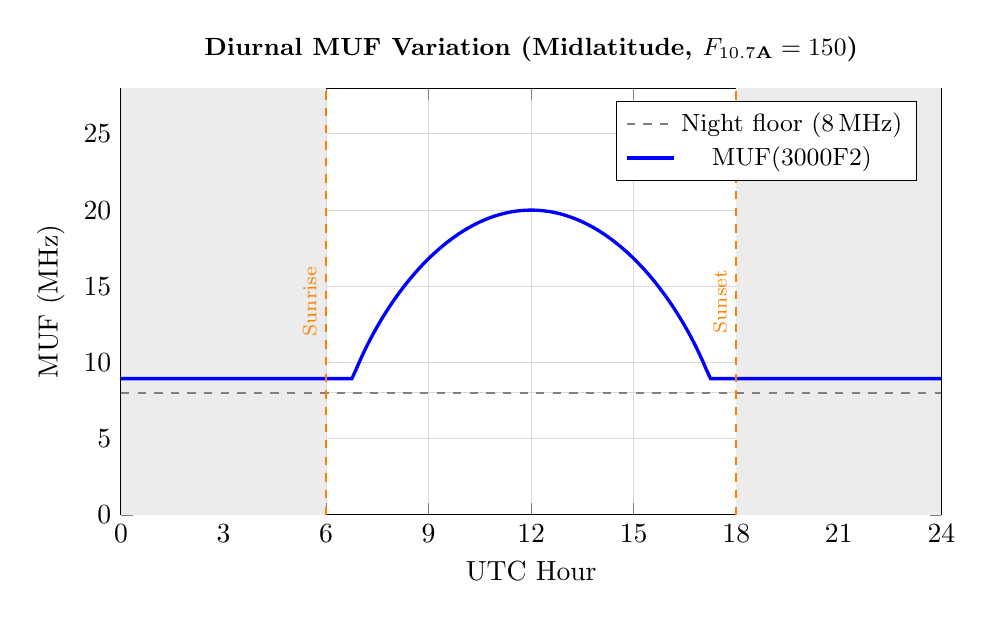
\begin{tikzpicture}
\begin{axis}[
  width=12cm, height=7cm,
  xlabel={UTC Hour},
  ylabel={MUF (\si{\MHz})},
  xmin=0, xmax=24,
  ymin=0, ymax=28,
  xtick={0,3,6,9,12,15,18,21,24},
  ytick={0,5,10,15,20,25},
  extra y ticks={8},
  extra y tick labels={},
  grid=major,
  grid style={gray!30},
  legend pos=north east,
  legend style={font=\small},
  title={Diurnal MUF Variation (Midlatitude, $F_{10.7\text{A}}=150$)},
  title style={font=\small\bfseries},
]

% Night floor at 8 MHz
\addplot[name path=floor,gray,dashed,thick,domain=0:24,samples=2]
  {8};
\addlegendentry{Night floor (\SI{8}{\MHz})}

% MUF curve: sqrt(cos(zenith)) shape, peak at local noon (12 UTC for this example)
% cos(chi) = sin(lat)*sin(dec) + cos(lat)*cos(dec)*cos(HA)
% Simplified: peak 20 MHz at noon, night floor 8 MHz
\addplot[name path=muf,blue,very thick,domain=0:24,samples=200]
  {max(8, 20 * max(0.447, sqrt(max(0.05, cos(deg(abs(x-12)/24*2*pi))))))};
\addlegendentry{MUF(3000F2)}

% Shade night region (before sunrise ~6, after sunset ~18)
\addplot[name path=xaxis,draw=none,domain=0:6,samples=2] {0};
\addplot[name path=top1,draw=none,domain=0:6,samples=2] {28};
\addplot[gray!15] fill between[of=xaxis and top1];

\addplot[name path=xaxis2,draw=none,domain=18:24,samples=2] {0};
\addplot[name path=top2,draw=none,domain=18:24,samples=2] {28};
\addplot[gray!15] fill between[of=xaxis2 and top2];

% Sunrise/sunset markers
\draw[orange,thick,dashed] (axis cs:6,0) -- (axis cs:6,28);
\node[font=\scriptsize,orange,anchor=south,rotate=90] at (axis cs:6,14) {Sunrise};
\draw[orange,thick,dashed] (axis cs:18,0) -- (axis cs:18,28);
\node[font=\scriptsize,orange,anchor=south,rotate=90] at (axis cs:18,14) {Sunset};

\end{axis}
\end{tikzpicture}
\caption{Diurnal MUF variation showing the $\sqrt{\cos\chi}$ shape
         scaled to a peak of \SI{20}{\MHz} (representative midlat
         $F_{10.7\text{A}} \approx 150$).  The dashed gray line at
         \SI{8}{\MHz} is the night-floor product
         $F \cdot \text{MUF}_{\text{peak}}$ from
         Eq.~\ref{eq:nightfloor}: $F$ is the dimensionless
         illumination ratio (${\sim}0.40$ at midlat moderate solar
         activity), which when applied to a \SI{20}{\MHz} daytime
         peak gives the \SI{8}{\MHz} floor curve plotted here.
         Shaded regions = night.}
\label{fig:mufdiurnal}
\end{figure}

% ═════════════════════════════════════════════════════════════════════
\section{Forward Projection (next 24\,h)}\label{sec:projection}

\begin{quote}\small\itshape
\textbf{Implementation status (entire section).}  The forward
projection pipeline described in this section --- MUF projection
(Eq.~\ref{eq:muffut}), seasonal ratio
(Section~\ref{sec:seasonalratio}), storm depression
(Section~\ref{sec:stormdepression}), sporadic-E persistence
(Section~\ref{sec:espersistence}), and gray-line bonus
(Section~\ref{sec:grayline}) --- is documented for a future build
of ionocast that exposes a projected outlook MUF as a first-class
display.  None of the \emph{forward-projection} pipeline currently
runs in the live runtime; the live runtime instead surfaces SWPC's
own next-72\,h forecasts on the Outlook panel.  Several of the
sub-pieces are however shared with the live budget --- specifically
$d(\cos\chi)$ (Eq.~\ref{eq:fof2-driver}), the storm-lag effective
$K_p$ (Section~\ref{sec:kplag}, which feeds $L_{\text{aur}}$ and
the $\sigma$-widening of Section~\ref{sec:tier-confidence} in the
\emph{live} pipeline), and the per-section ``Implementation status''
insets call those out individually.  Read this section's equations
as the form a future outlook-MUF display would use, not as
forward-tense equations whose absence from runtime makes them
operationally inert: the parts that touch the live pipeline are
already running.
\end{quote}

The forward projection engine extends the current nowcast into the
future by modelling the dominant drivers of ionospheric change.

\subsection{MUF Projection via Solar Zenith Analogy}\label{sec:muf-now-vs-future}

\begin{equation}\label{eq:muffut}
  \text{MUF}_{\text{future}} = \text{MUF}_{\text{now}} \cdot
    \frac{S(d(\cos\chi_{\text{future}}),\, F)}{S(d(\cos\chi_{\text{now}}),\, F)}
    \cdot R_{\text{seasonal}} \cdot \frac{F_{\text{storm}}(K_p^{\text{fut}})}
                                          {F_{\text{storm}}(K_p^{\text{now}})}
\end{equation}
where $K_p^{\text{fut}}$ is the SWPC 3-day forecast value at
$t + \Delta$ (or the current $K_p$ when $\Delta = 0$).  Both the
``now'' and ``future'' zenith arguments pass through the same
3-hour memory-lag function $d(\cos\chi)$ defined in
Eq.~\ref{eq:fof2-driver} (Section~\ref{sec:climo}); using raw
$\cos\chi$ on either side without the lag would produce a
discontinuity at the projection's $\Delta = 0^+$ boundary
relative to the live nowcast (which already runs through
$d(\cos\chi)$), most visibly at sunset where the live model holds
foF2 elevated for ${\sim}3$\,h via memory while a raw-cos$\chi$
projection would drop it instantly.  The storm factor enters as a
\emph{ratio} so the projection only adjusts for the \emph{change}
in storm phase between now and the projection horizon: if the
current $K_p$ already encodes the disturbance,
$\text{MUF}_{\text{now}}$ is already depressed and the ratio is
near unity; if a storm is forecast to arrive within $\Delta$ but
hasn't yet, $K_p^{\text{fut}} > K_p^{\text{now}}$ depresses the
projection accordingly. This complements the $\sigma$-side
forecast bump in Section~\ref{sec:reliability} (which widens
$\sigma$ ahead of a forecast disturbance) by adjusting the
deterministic mean as well; together they avoid the failure mode
where $\text{MUF}_{\text{now}}$ encodes a quiet ionosphere but a
storm has been forecast for the horizon.

\paragraph{Implementation status.}  As with $F_{\text{storm}}$,
the forward-projection MUF is documented but not currently wired
into a real-time display in the runtime build.  The live verdict
uses $\text{MUF}_{\text{now}}$ (with $d(\cos\chi_{\text{now}})$)
directly; no projection chart is exposed.  When that chart is
wired, the equation above is the form to use, with $d(\cos\chi)$
on both sides of the ratio.

\subsection{Seasonal Ratio}\label{sec:seasonalratio}

\begin{equation}
  R_{\text{seasonal}} = \frac{s(t_{\text{future}},\,\phi)}{s(t_{\text{now}},\,\phi)}
\end{equation}
where
\begin{equation}\label{eq:seasonal}
  s(t,\phi) = 1 + (0.15\cos\theta + 0.08\cos(2\theta + \pi))
              \cdot w(\phi)
\end{equation}
with $\theta = 2\pi\,(d_{\text{yoy}} - d_{\text{solstice}})/365$,
where $d_{\text{yoy}}$ is the UTC day of year ($1 = 1$~January) and
$d_{\text{solstice}}$ is the local-hemisphere winter-solstice day:
$d_{\text{solstice}} = 355$ (December~21) for $\phi \geq 0$ and
$d_{\text{solstice}} = 172$ (June~21) for $\phi < 0$.  The
day-of-year phase places the cosine peak at the astronomical
solstice; an earlier calendar-month formulation
$\theta_m = 2\pi\,(m + 0.5 - m_{\text{winter}})/12$ landed the peak
five days early (Dec~16 vs Dec~21 in the NH) because mid-month does
not coincide with the solstice date.  This formulation matches
Eq.~\ref{eq:winter} in the climatology so the two seasonal effects
share the same phase reference.  $w(\phi) =
\min(1, |\phi|/50)$ scales the modulation toward midlatitudes. The
first term captures the annual winter-peak/summer-trough at
midlatitudes; the second captures the semi-annual equinox peaks
(March, September) evident in F2-layer statistics.  This formula
shares the mid-month phase convention with the winter-anomaly term
in Eq.~\ref{eq:winter} so the two seasonal effects --- which
overlap in the annual component --- align rather than drifting two
weeks apart.

\begin{figure}[H]
\centering
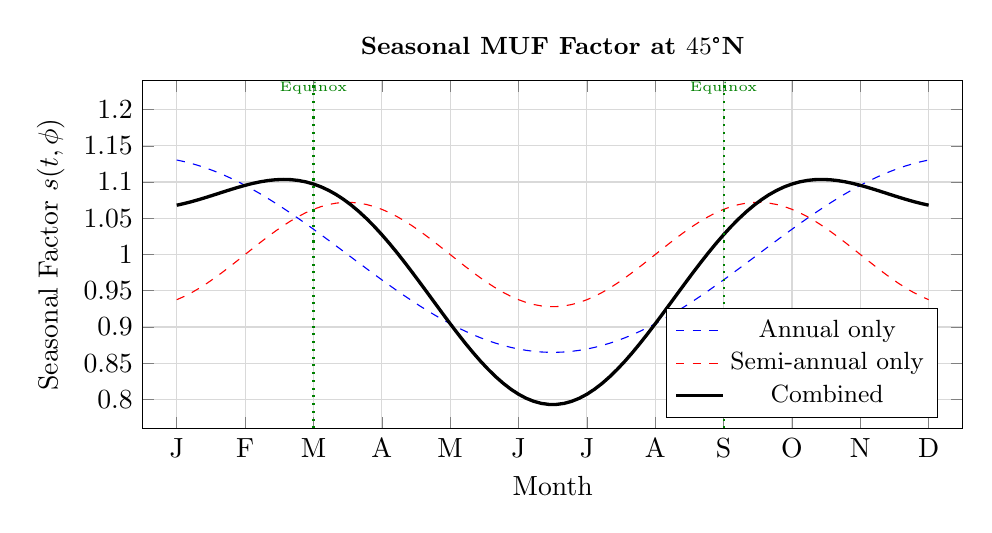
\begin{tikzpicture}
\begin{axis}[
  width=12cm, height=6cm,
  xlabel={Month},
  ylabel={Seasonal Factor $s(t,\phi)$},
  xmin=0.5, xmax=12.5,
  ymin=0.76, ymax=1.24,
  xtick={1,2,3,4,5,6,7,8,9,10,11,12},
  xticklabels={J,F,M,A,M,J,J,A,S,O,N,D},
  ytick={0.80,0.85,0.90,0.95,1.00,1.05,1.10,1.15,1.20},
  grid=major,
  grid style={gray!30},
  legend pos=south east,
  legend style={font=\small},
  title={Seasonal MUF Factor at $45\text{\textdegree}$N},
  title style={font=\small\bfseries},
]

% s(t,phi) = 1 + (0.15*cos(theta) + 0.08*cos(2*theta + pi)) * w
% theta = 2*pi*(m + 0.5 - m_winter)/12, m_winter=0 (Jan) for NH
% m = x-1 (x is 1-indexed month), so theta = 2*pi*((x-1)+0.5)/12 = pi*(x-0.5)/6
% w(45) = min(1, 45/50) = 0.9
% NH peak at theta=0: x-0.5=0 -> x=0.5, i.e. mid-December ✓

% Annual component only
\addplot[blue,dashed,domain=1:12,samples=100]
  {1 + 0.15*cos(deg((x-0.5)*pi/6)) * 0.9};
\addlegendentry{Annual only}

% Semi-annual only
\addplot[red,dashed,domain=1:12,samples=100]
  {1 + 0.08*cos(deg(2*(x-0.5)*pi/6 + pi)) * 0.9};
\addlegendentry{Semi-annual only}

% Combined
\addplot[black,very thick,domain=1:12,samples=100]
  {1 + (0.15*cos(deg((x-0.5)*pi/6)) + 0.08*cos(deg(2*(x-0.5)*pi/6 + pi))) * 0.9};
\addlegendentry{Combined}

% Equinox markers
\draw[green!50!black,thick,dotted] (axis cs:3,0.76) -- (axis cs:3,1.24);
\draw[green!50!black,thick,dotted] (axis cs:9,0.76) -- (axis cs:9,1.24);
\node[font=\tiny,green!50!black] at (axis cs:3,1.23) {Equinox};
\node[font=\tiny,green!50!black] at (axis cs:9,1.23) {Equinox};

\end{axis}
\end{tikzpicture}
\caption{Seasonal MUF factor at $45\text{\textdegree}$N showing annual
         (winter peak) and semi-annual (equinox peaks) components.
         At $|\phi| = 45\text{\textdegree}$, $w(\phi) = 45/50 = 0.9$,
         so the annual component reaches $1 + 0.15 \cdot 0.9 = 1.135$
         in isolation at the winter solstice and the semi-annual
         component reaches $1 + 0.08 \cdot 0.9 = 1.072$ in isolation at
         the equinoxes.  Because the two components compete at the
         winter solstice --- the semi-annual is at its trough there
         (\,$\cos(2\theta + \pi) = -1$ at $\theta = 0$\,) --- the
         combined curve is flatter than either component alone: the
         winter solstice evaluates to $1 + (0.15 - 0.08) \cdot 0.9 =
         1.063$, the March / September equinoxes to $1 + 0.08 \cdot
         0.9 = 1.072$, and the summer solstice to $1 - (0.15 + 0.08)
         \cdot 0.9 = 0.793$.  The dominant seasonal feature at this
         latitude is therefore the deep summer trough rather than a
         sharp winter peak; winter and equinoxes form a broad plateau
         in the $1.06$--$1.07$ range, with the equinoxes slightly
         above the winter solstice ($+0.009$).  Above $|\phi| =
         50\text{\textdegree}$ the weight saturates at $w = 1$ and the
         summer trough deepens to $0.77$ while the winter / equinox
         plateau settles at $1.07$--$1.08$.}
\label{fig:seasonal}
\end{figure}

\subsection{Storm Depression (forward-projection definition)}\label{sec:stormdepression}

The forward-projection storm depression follows the F-region storm
phenomenology surveyed by Pr\"olss~\cite{prolss1995}, Fuller-Rowell
et al.~\cite{fullerrowell1994}, and Mendillo~\cite{mendillo2006}: a
prompt depression of foF2 driven by Joule heating of the
thermosphere and the resulting O/N$_2$ composition shift, with a
recovery timescale set by the storm's driver (impulsive CME vs
sustained HSS).

\begin{quote}\small\itshape
\textbf{Implementation status.}  The expressions in this subsection
define the $F_{\text{storm}}$ multiplier referenced by Eq.~\ref{eq:muffut}
(the forward-projection MUF for the outlook section). The
\emph{current-time} MUF in production does \emph{not} apply this
multiplier: the runtime budget reflects geomagnetic storm response
through the storm-lagged effective $K_p$ feeding $L_{\text{aur}}$
(Section~\ref{sec:laur} and Section~\ref{sec:kplag}), not as a
MUF-side scalar.  $F_{\text{storm}}$ as a real-time MUF multiplier
is reserved for a future build that exposes the projected outlook
MUF as a first-class display.
\end{quote}

When $K_p > 4$, the projected MUF is depressed; for $K_p \le 4$ the
factor holds at unity (no quiet-day boost):
\begin{equation}\label{eq:storm}
  F_{\text{storm}} = \max\!\left(F_{\text{floor}}(K_p),\;
    1 - p\,\max(0,\,K_p - 4)\right)
\end{equation}
where
\begin{equation}
  p = 0.05 + 0.10 \cdot \text{clamp}\!\left(
    \frac{|\phi_{\text{CGM}}| - 40}{30},\;0,\;1\right)
\end{equation}
The two latitude anchors place the slope ramp where the underlying
F-region storm physics actually transitions.  $|\phi_{\text{CGM}}| =
40\degree$ is the ceiling of the trough region during strong storms
in cycle-25 Dst-vs-foF2 records (Mendillo~\cite{mendillo2006};
Pr\"olss~\cite{prolss1995}): below this, the storm-time foF2 depression
is dominated by composition-shift effects whose magnitude is well
captured by a gentle $p = 0.05$.  $|\phi_{\text{CGM}}| = 70\degree$
is the equatorward edge of the auroral oval at $K_p \approx 7$
(the storm-zone expansion threshold of
Eq.~\ref{eq:auroralexpansion}'s converged state); poleward of it,
the F-region sees direct precipitation-driven heating in addition
to the global thermospheric shift, and a steeper $p = 0.15$ matches
the ${\sim}50\%$ MUF collapses observed in IRI-validated ground
campaigns.  The $30\degree$ ramp width connects them linearly; this
is geometric interpolation rather than a separate physics prediction.
The floor itself drops below 0.5 during severe storms to capture
the deep MUF collapse documented for $K_p \geq 8$ events:
\begin{equation}\label{eq:stormfloor}
  F_{\text{floor}}(K_p) = \max\!\Bigl(
    0.30,\; 0.50 - 0.10 \cdot \min\!\bigl(2,\,\max(0,\,K_p - 7)\bigr)
  \Bigr)
\end{equation}
At quiet to moderate $K_p$ the floor is at 0.5 (50\% of quiet
baseline). At $K_p = 8$ (G4) it drops to 0.4; at $K_p = 9$ (G5)
it drops to 0.3.  The crossover $K_p$ at which the floor binds
(i.e.\ the main term drops below the floor schedule) is
\begin{equation}\label{eq:stormfloorcross}
  K_p^{*} = 4 + \frac{1 - F_{\text{floor}}(K_p^{*})}{p}
\end{equation}
which evaluates to exactly $8.0$ on auroral paths
($p = 0.15$, $|\phi_{\text{CGM}}| \ge 70\degree$) --- so for
$K_p \ge 8.0$ the floor schedule binds at polar latitudes
(at $K_p = 8$ both the main term $1 - 0.15 \cdot 4 = 0.40$ and
the floor $0.50 - 0.10 \cdot 1 = 0.40$ coincide; at $K_p = 9$
the main term gives $1 - 0.15 \cdot 5 = 0.25$, the floor gives
$0.50 - 0.10 \cdot 2 = 0.30$, and $\max(0.30, 0.25) = 0.30$).  At midlatitude paths the slope
$p = 0.05$ keeps the main term above the floor for any
plausible $K_p$ ($K_p^{*} \approx 18$ at $|\phi_{\text{CGM}}|
= 40\degree$, far past the $K_p = 9$ ceiling), so the floor
schedule \emph{never binds at midlat} and the floor refinement
is auroral-only by construction.  The earlier flat 0.5 floor
under-predicted severity during real super-storms (Halloween
2003, March 1989) where polar F2 MUF fell below 50\% of baseline
for hours, which the new schedule captures only on the auroral
paths it actually applied to.

At midlatitudes ($|\phi_{\text{CGM}}| = 40\text{\textdegree}$), the
damping is 5\%~per~$K_p$ unit above~4.  In the auroral zone
($|\phi_{\text{CGM}}| = 70\text{\textdegree}$), it rises to
${\sim}15$\% per unit.

\paragraph{Negative phase only.}  $F_{\text{storm}}$ models the
\emph{negative-phase} F-region storm response (the persistent
electron-density depression caused by neutral composition changes
and Joule heating that lasts hours-to-days into the storm main and
recovery phases).  It does not model the brief \emph{positive
phase} that can precede the depression in the first
${\sim}30$--$60$\,min after a sudden CME impact, where neutral
composition changes and ionospheric heating can transiently
\emph{enhance} foF2 by 10--20\,\%.  The result is that the model
under-predicts MUF in the very early phase of a fast-onset CME
event (a quiet-time prediction is correct; the depression engages
correctly within an hour or two).  In practice this matters only
for operators chasing the rare positive-phase opening on the
upper bands during the first hour of a sudden storm, which is a
boutique mode --- the negative-phase damping that follows is what
shapes the bulk of the storm-affected propagation window.  When the
projected-MUF panel ships (currently documented but not yet
surfaced --- see implementation status above), it should carry an
annotation flagging this gap, paralleling how the scatter
(\S\ref{sec:scatter}) and TEP (\S\ref{sec:tep}) modes are tagged on
the verdict line.  Until then, operators tracking a fresh CME
should trust the alerts-panel $B_z$ / $D_{\text{st}}$ / PCA chips
for the impact signal rather than expecting the projection to flip
positive in the first hour.

\subsubsection{Storm-Lag Effective $K_p$}\label{sec:kplag}

The F-region does not respond instantaneously to the $K_p$ kick: Joule
heating of the thermosphere and subsequent composition changes take
1--3\,hours to depress the peak electron density, and the ionosphere
then recovers over the following 12--24\,hours.  Feeding the raw
instantaneous $K_p$ into the physics budget therefore mis-times both
the onset and the recovery of a storm.

ionocast builds an exponentially-weighted \emph{effective} $K_p$ from
the 7-day SWPC $K_p$ history (3-hour cadence), peaked at
$\tau_{\text{peak}} = \SI{2}{\hour}$ in the past with a decay constant
$\tau_{\text{decay}}$ that depends on the storm's driver:
\begin{equation}\label{eq:kplag}
  K_p^{\text{eff}} = \frac{
    \sum_i K_p(t_i)\,
    \exp\!\bigl(-|\Delta t_i - \tau_{\text{peak}}|/\tau_{\text{decay}}\bigr)
  }{
    \sum_i \exp\!\bigl(-|\Delta t_i - \tau_{\text{peak}}|/\tau_{\text{decay}}\bigr)
  }
\end{equation}
with $\Delta t_i = t_{\text{now}} - t_i$ (positive for past samples).

\paragraph{Storm-type classification.}  CME-driven and CIR / HSS-driven
storms recover on very different timescales.  A CME arrival is an
impulse: after the shock and main phase, Joule heating dissipates
over ${\approx}\SI{8}{\hour}$.  A co-rotating interaction region
(CIR) or high-speed stream (HSS) is a sustained driver that keeps
heating the thermosphere while the stream flows past Earth -- recovery
takes ${\approx}\SI{24}{\hour}$ or longer.  ionocast picks the kernel
as follows:
\begin{itemize}[nosep]
  \item If $\text{Dst} < -\SI{80}{nT}$ the ring current is deep: CME
        signature dominates, $\tau_{\text{decay}} = \SI{8}{\hour}$.
        (If $\text{Dst}$ is unavailable from the upstream feed,
        skip to the next branch rather than treating the missing
        value as $\geq -\SI{80}{nT}$.)
  \item Otherwise, if NASA DONKI~\cite{donki} reports an HSS event within the last
        \SI{24}{\hour} or next \SI{48}{\hour}, use
        $\tau_{\text{decay}} = \SI{24}{\hour}$.  The asymmetric
        window is intentional: DONKI's HSS analyses are typically
        published within hours of stream onset (so a 24-hour
        lookback covers events the catalogue has already classified)
        but stream peak effects on the magnetosphere can lag the
        L1 arrival by 12--36\,hours and persist for another
        12--24\,hours, so a 48-hour lookahead extends the
        24-hour-decay regime through the stream's effective
        magnetospheric tail.
  \item Otherwise default to $\tau_{\text{decay}} = \SI{8}{\hour}$.
\end{itemize}
Only $K_p^{\text{eff}}$ enters the physics; the UI still displays the
instantaneous sample so the shown number matches SWPC's feed.

\subsubsection{Dst, IMF Bz, and Solar-Wind Drivers}\label{sec:fast-storm-drivers}

The 3-hour Kp index is a lagging indicator.  Three faster-responding
inputs are wired into the storm model:

\begin{itemize}[nosep]
  \item \textbf{Dst} (Kyoto ring-current index): when $\text{Dst} < -50$\,nT,
        the effective $K_p$ is bumped by up to $+2$ (1 per 50\,nT below $-50$).
        Dst responds within minutes of storm onset, 1--3 hours before Kp updates.
  \item \textbf{IMF Bz forward bump} (DSCOVR/ACE L1 solar wind): the
        L1 monitor sits ${\sim}\SI{1.5e6}{km}$ upstream, giving a
        nominal 30--60\,min lead on the geomagnetic effect at
        Earth (the spread on the lead time depends on solar-wind
        speed: $\SI{1.5e6}{km} / \SI{400}{km/s} = 62$\,min at
        average speeds, $\SI{1.5e6}{km} / \SI{800}{km/s} = 31$\,min
        at fast streams).  The L1-to-Earth correlation is
        \emph{probabilistic}, not deterministic: not every L1-observed
        Bz dip arrives at Earth's magnetopause unchanged --- some
        structures are spatially extended and miss Earth entirely
        ($Y_{\text{GSE}} \neq 0$), some glance the magnetopause
        without sustained reconnection, and some get reshaped by
        intermediate solar-wind structures during transit.  The
        20-min median is gated at $-5$\,nT: medians at or above
        $-5$\,nT (i.e.\ $B_z \geq -5$) produce no bump; medians
        strictly below $-5$\,nT (i.e.\ $B_z < -5$) ramp the bump per
        Table~\ref{tab:bzbump}.  The cutoff filters out short
        reconnection bursts that don't drive sustained magnetopause
        coupling, but the L1 forward bump should be treated as an
        early-warning probability bump on the effective $K_p$, not
        a guaranteed forecast.  When the median Bz over the last
        20 min is sustained below threshold, the effective $K_p$ is
        bumped additively \emph{before} the index reading catches
        up (Table~\ref{tab:bzbump}); single-sample dips below
        threshold do not count.  The bump decays to zero once
        $B_z$ returns to $\geq -5$\,nT.
  \item \textbf{Solar-wind plasma} (DSCOVR/ACE): sustained speed
        $\geq \SI{500}{km/s}$ with sharply negative Bz
        ($\leq -8$\,nT) is read as a CME shock arrival regardless of
        DONKI catalogue inertia, while the same speed with mild Bz
        ($> -5$\,nT) is read as HSS / corotating-stream interaction.
        The intermediate regime (\SI{500}{km/s} or faster with
        $-8 < B_z \le -5$\,nT) is ambiguous in the live signal ---
        moderate southward Bz with elevated speed could be either
        the leading edge of a CME sheath or sustained HSS-driver
        reconnection --- so neither shortcut fires; the classifier
        falls through to the catalogue / Dst logic below, which
        defaults to the CME timescale ($\tau_{\text{decay}} =
        \SI{8}{h}$) unless an active DONKI HSS event covers the
        current window.  Storm-type classification picks the decay
        time-scale ($\tau_{\text{decay}} = \SI{8}{h}$ vs.\
        \SI{24}{h}) of the Section~\ref{sec:kplag} kernel.
\end{itemize}

All adjustments are capped at $K_p = 9$ and apply only when the
respective input is available.  The auroral CGM threshold expands
continuously from $60\degree$ (quiet, $K_p \le 5$) to $50\degree$
(severe, $K_p \ge 7$), per Eq.~\ref{eq:auroralexpansion} ---
linear in $K_p$ across the $5 \to 7$ window so the equatorward
expansion of the auroral oval enters the budget gradually rather
than stepping at a single threshold.

\begin{table}[H]
\centering
\caption{Effective $K_p$ bump from a sustained southward-Bz median
         observed at the L1 monitor (DSCOVR / ACE) over the trailing
         20 minutes. The function is a continuous linear ramp from
         0 at $B_z = -5$\,nT to $+3$ at $B_z = -15$\,nT, saturating
         at $+3$ for deeper southward IMF. Table values are sample
         points along the ramp.}
\label{tab:bzbump}
\begin{tabular}{@{}lr@{}}
\toprule
\textbf{Median Bz over 20 min} & \textbf{$K_p$ bump} \\
\midrule
$\geq -5$\,nT   & $0$            \\
$-6$\,nT        & $+0.3$         \\
$-10$\,nT       & $+1.5$         \\
$-12$\,nT       & $+2.1$         \\
$-15$\,nT       & $+3$ (saturated) \\
$\leq -15$\,nT  & $+3$ (saturated) \\
\bottomrule
\end{tabular}
\end{table}
Earlier table form had stepped thresholds at $-5 / -10 / -15$\,nT
producing a $+1$\,Kp jump on every threshold crossing --- same
family of cliff as the auroral Kp gate, the storm-zone CGM
expansion, and the X-ray flare twilight gate retired in the
2026-04 polish round.  The continuous ramp closes that.

\begin{figure}[H]
\centering
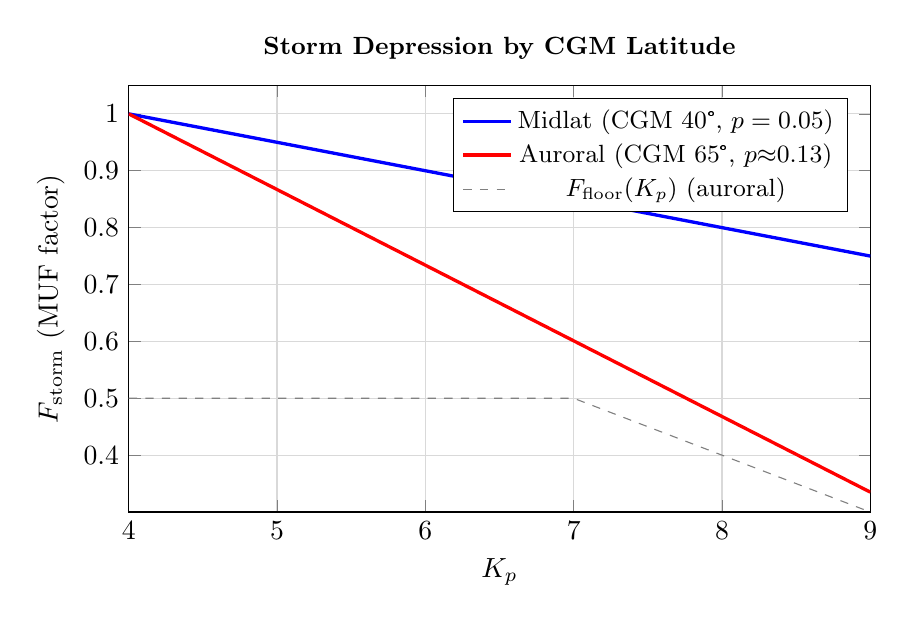
\begin{tikzpicture}
\begin{axis}[
  width=11cm, height=7cm,
  xlabel={$K_p$},
  ylabel={$F_{\text{storm}}$ (MUF factor)},
  xmin=4, xmax=9,
  ymin=0.3, ymax=1.05,
  xtick={4,5,6,7,8,9},
  ytick={0.4,0.5,0.6,0.7,0.8,0.9,1.0},
  grid=major,
  grid style={gray!30},
  legend pos=north east,
  legend style={font=\small},
  title={Storm Depression by CGM Latitude},
  title style={font=\small\bfseries},
]

% Ffloor(Kp) = max(0.30, 0.50 - 0.10*min(2, max(0, Kp-7)))
% Midlat: CGM = 40°, p = 0.05 + 0.10*clamp((40-40)/30,0,1) = 0.05
% Midlat floor: Ffloor never binds (K*_p ~18), so max(0.5,...) is correct here
\addplot[blue,very thick,domain=4:9,samples=50]
  {max(0.5, 1 - 0.05*(x-4))};
\addlegendentry{Midlat (CGM $40\text{\textdegree}$, $p=0.05$)}

% Auroral: CGM = 65°, p = 0.05 + 0.10*clamp((65-40)/30,0,1) = 0.05 + 0.10*0.833 = 0.133
% Auroral floor: Ffloor drops to 0.40 at Kp=8 and 0.30 at Kp=9 (Eq. stormfloor)
\addplot[red,very thick,domain=4:9,samples=200]
  {max(max(0.30, 0.50 - 0.10*min(2, max(0, x-7))), 1 - 0.133*(x-4))};
\addlegendentry{Auroral (CGM $65\text{\textdegree}$, $p{\approx}0.13$)}

% Ffloor schedule reference line (auroral only)
\addplot[gray,dashed,domain=4:9,samples=200]
  {max(0.30, 0.50 - 0.10*min(2, max(0, x-7)))};
\addlegendentry{$F_{\text{floor}}(K_p)$ (auroral)}

\end{axis}
\end{tikzpicture}
\caption{Storm MUF depression factor vs.\ $K_p$ for midlatitude and
         auroral-zone paths.  The midlatitude floor never binds (slope
         $p=0.05$ keeps the main term above 0.5 for all $K_p \le 9$).
         The auroral curve plotted is at $|\phi_{\text{CGM}}| =
         65\degree$ (where the slope $p \approx 0.13$ is not yet at
         its $|\phi_{\text{CGM}}| \ge 70\degree$ ceiling of $0.15$);
         the floor schedule
         $F_{\text{floor}}(K_p)$ (Eq.~\ref{eq:stormfloor})
         drops from 0.5 at $K_p < 7$ to 0.40 at $K_p=8$ and 0.30
         at $K_p=9$ but only \emph{just} starts to bind on this
         curve at $K_p \approx 9$.  The clean ``main term and floor
         coincide at 0.40 at $K_p = 8$'' result discussed in
         Eq.~\ref{eq:stormfloorcross} applies at
         $|\phi_{\text{CGM}}| \ge 70\degree$, not at the
         65\textdegree{} curve plotted here.}
\label{fig:storm}
\end{figure}

\subsection{Sporadic-E Persistence}\label{sec:espersistence}

The projected critical frequency of the sporadic-E layer decays
exponentially:
\begin{equation}\label{eq:es}
  f_{\text{oEs}}(t + \Delta) = \max\!\left(B(\cos\chi),\;
    f_{\text{oEs}}(t) \cdot 2^{-\Delta/\tau(\cos\chi)}\right)
\end{equation}
with the half-life and floor smoothly interpolated across the
twilight band $\cos\chi \in [0.1, 0.3]$ rather than stepped at a
single $\cos\chi = 0.2$ threshold (the earlier formulation produced
a $2\times$ jump in $\tau$ and a 2 MHz jump in $B$ at the threshold,
which on a band gated by $f \le 5 f_{\text{oEs}}$ translated to a
$10\,\text{MHz}$ step in the gating threshold --- same family of
cliff retired by the auroral and Bz onset ramps in
Section~\ref{sec:laur}).  The interpolated forms are
\begin{equation}
  \tau(\cos\chi) = \SI{1.5}{\hour} +
    \SI{1.5}{\hour}\cdot\sigma\!\left(\tfrac{\cos\chi - 0.1}{0.2}\right),
  \qquad
  B(\cos\chi) = \SI{2}{\MHz}\cdot\sigma\!\left(\tfrac{\cos\chi - 0.1}{0.2}\right)
\end{equation}
where $\sigma(x) = \mathrm{clamp}(x, 0, 1)$ is a unit ramp.  At
$\cos\chi \le 0.1$ both reduce to their night values
($\tau = 1.5\,\text{h}$, $B = 0$); at $\cos\chi \ge 0.3$ both
saturate to the day values ($\tau = 3.0\,\text{h}$, $B = 2\,\text{MHz}$).
At deep twilight ($\cos\chi = 0.2$) the function is at midpoint
($\tau = 2.25\,\text{h}$, $B = 1\,\text{MHz}$), and the band-MUF
gating threshold transitions continuously rather than stepping.

This subsection describes the documented forward-projection
persistence model; it is part of the deferred outlook MUF
projection (Section~\ref{sec:muf-now-vs-future}) and is not
exercised by the live runtime budget at $t = 0$.

\subsection{Gray-Line Bonus (Asymmetric)}\label{sec:grayline}

When the reflection midpoint lies near the solar terminator
($|\cos\chi| < 0.1$) the D-region is thin, so a small additive
bonus is applied to the margin.  The effect is strongest on the
low bands --- where D-region absorption normally dominates the
budget --- and fades away by the upper HF.  Sunrise and sunset are
treated \emph{asymmetrically}: at dawn, the D-region has not rebuilt
yet while the F-region has started ionising, so the low-band window
is long and clean; at dusk, the D-region decays more slowly than the
residual F-region enhancement, producing a shorter and weaker window.
Sunrise is distinguished from sunset by the sign of
$\mathrm{d}\cos\chi/\mathrm{d}t$, sampled 5\,minutes ahead.  This
sign-based distinction is meaningful only \emph{near the terminator}
($|\cos\chi| < 0.1$, the bonus's proximity gate $p$ above): at any
location the cosine derivative $\mathrm{d}\cos\chi/\mathrm{d}t$ is
positive throughout the morning half-day from local midnight to
local noon (so the sign alone does not identify sunrise everywhere
in that range), but the proximity gate restricts the bonus to the
small window where $\cos\chi$ is near zero, and within that
window the morning side is genuine sunrise and the evening side
is genuine sunset --- the sign correctly discriminates the two
\emph{at the terminator} even though it does not in general:
\begin{equation}\label{eq:gl}
  B_{\text{GL}}(f) = B_{\text{band}}(f, \mathrm{phase})\cdot p
\end{equation}
where the per-band amplitude depends on the terminator phase
(sunrise vs sunset) per Table~\ref{tab:graylineamps}.

\begin{table}[H]
\centering
\caption{Gray-line bonus amplitude in dB by band and terminator phase.}
\label{tab:graylineamps}
\begin{tabular}{@{}l c c@{}}
\toprule
\textbf{Band} & \textbf{Sunrise (dB)} & \textbf{Sunset (dB)} \\
\midrule
160\,m, 80\,m              & 6   & 3   \\
60\,m, 40\,m               & 5   & 3   \\
30\,m                      & 3   & 1.5 \\
20\,m                      & 1.5 & 1.0 \\
17\,m and above            & 0   & 0   \\
\bottomrule
\end{tabular}
\end{table}

Proximity $p = 1 - \min(1, |\cos\chi|/0.1)$ scales
the bonus linearly from zero at $|\cos\chi| = 0.1$ to full amplitude
at the terminator.  Above \SI{14}{\MHz} the D-region contributes
little, so no bonus is modelled.

\paragraph{Midpoint vs.\ per-hop evaluation.}  The proximity
$|\cos\chi|$ is computed at the reflection \emph{midpoint} only,
not at each hop along the great circle.  This is a deliberate
simplification: the D-region absorption \emph{loss} term
(Eq.~\ref{eq:labsd-path}) is evaluated per-hop and summed, but the
gray-line \emph{bonus} compensates loss at the terminator, and
on a 4-hop transatlantic path whose midpoint sits in midday but
whose terminus hop is at sunrise the per-hop loss already drops on
that one hop's $L_{\text{Dreg}}$ contribution; adding a
midpoint-only bonus on top would over-count the local effect on
the geometric-midpoint hop while under-counting the genuine
sunrise hops at the path ends.  The midpoint-only formulation
captures the case the bonus is operationally intended for ---
short-to-medium HF paths (1--2 hops, 1500--6000\,km) whose single
or twin reflection points cross the terminator together, where
``the path is on the gray line'' and ``the midpoint is at the
terminator'' coincide.  For longer multi-hop paths (5000\,km+)
where one terminus is in daylight and the other near sunrise, the
per-hop $L_{\text{Dreg}}$ already does the right thing on its own.
Extending the bonus to a per-hop max is a candidate refinement
tracked in Section~\ref{sec:limits}; today's midpoint-only form
is simpler to reason about and avoids the over-count.

% ═════════════════════════════════════════════════════════════════════
\section{Alternative Propagation Modes}\label{sec:altprop}

The F2-layer SNR budget (Section~\ref{sec:snr}) is the default path
for every HF circuit, but four additional modes can open bands that
the F2 budget marks closed: sporadic-E (\S\ref{sec:es-prop-mode}),
trans-equatorial propagation (\S\ref{sec:tep}), meteor scatter
(\S\ref{sec:ms}), and F2-region scatter recovery
(\S\ref{sec:scatter}).  Each runs in parallel with the F2 budget on
the same path set; the verdict takes whichever mode has the best
margin.  Tropospheric ducting (\S\ref{sec:tropo}) is also covered
in this section but is structurally different --- it is surfaced as
a measured per-station panel rather than folded into the budget,
because a duct's spatial extent is not resolved by the sparse
radiosonde basket the gradient is computed from.

\subsection{Sporadic-E as a Propagation Mode}\label{sec:es-prop-mode}

The Es-screening term ($L_{\text{Es}}$, Section~\ref{sec:snr}) only
accounts for Es \emph{blocking} an F2 hop.  In reality Es can itself
be the propagation mode (the framework for which is ITU-R
P.534~\cite{itup534}): a single ${\sim}\SI{2000}{\km}$ hop off the
E layer at ${\sim}\SI{110}{\km}$ altitude, with no F2 variability and
no auroral absorption.  This is the mechanism behind summer-evening
15\,m, 12\,m, 10\,m, and 6\,m openings that the F2-only model would
otherwise call closed.  6\,m only opens via Es when $f_{\text{oEs}}
\gtrsim \SI{10}{\MHz}$ (so that $5\,f_{\text{oEs}} \ge \SI{50}{\MHz}$),
which is rarer than the HF-band thresholds and concentrated in the
boreal-summer Es season.

ionocast defines a sporadic-E budget alongside the F2 one:
\begin{equation}\label{eq:esmargin}
  M_{\text{Es}} = P_{\text{tx}} + G_{\text{ant}}
    - L_{\text{fs}}(f, d_{\text{Es}})
    - L_{\text{Dreg}} - L_{\text{PCA}} - L_{\text{flare}}
    - L_{\text{MUF,Es}}(f, 5 f_{\text{oEs}})
    - L_{\text{iono,Es}} - L_{\text{low}}
    - N - S_{\text{req}}
\end{equation}
with $d_{\text{Es}} = \SI{2000}{\km}$, a single-hop takeoff angle
$\approx\!6.3\degree$, and $L_{\text{iono,Es}} = \SI{15}{\dB}$.

\paragraph{What's in $L_{\text{iono,Es}} = \SI{15}{\dB}$.} Substantially
larger than the F2 lumped term $L_{\text{iono}} = \SI{1}{\dB}$
(Section~\ref{sec:liono}) because the E-layer reflection geometry
introduces several mechanisms a clean F2 reflection does not:
patchy cloud structure (footprint mismatch between TX and RX
illumination), strong aspect sensitivity at the layer's tilted
surfaces, polarisation scrambling through a thin gradient layer,
and substantial residual ITU-R Yp population variability since Es
strength swings hour-to-hour rather than the F2 spread that the
P.533 day-to-day budget captures. Future calibration may
redistribute this into named per-mechanism terms; the lumped 15 dB
is the empirical equivalent.

The D-region terms still apply --- the E layer sits above the D
layer, so an Es signal still passes the absorbing region once per
hop.  $L_{\text{hop}}$ is zero for Es (single-hop, no intermediate
ground reflections).  $L_{\text{aur}}$ is \emph{omitted} from
Eq.~\ref{eq:esmargin} entirely (the term is not in the equation),
\emph{not} because it can't physically apply --- it can; auroral D
absorption affects any signal traversing the D-region, and Es
hops cross the D-region twice (TX up, down to RX) --- but because
the geographic regions where Es is the dominant propagation mode
overlap rarely with the auroral oval.  The $f \geq \SI{14}{\MHz}$
operating range and summer-evening seasonality of strong Es push
most Es hops to midlat / equatorial corridors away from the
auroral CGM threshold.  On the rare auroral-zone summer-Es path
(Scandinavia, Alaska, Antarctic) where both mechanisms co-occur
the budget under-predicts absorption; treat ``$L_{\text{aur}} = 0$
on Es'' as a geographic simplification rather than a physical
claim.

Gating in code: \texttt{snrMarginHfEs} returns null below
\SI{14}{\MHz} regardless of $f_{\text{oEs}}$
(\texttt{src/physics/snr.js}), even though the algebraic Es MUF
gate $f \le 5 f_{\text{oEs}}$ would otherwise admit lower bands
on strong Es days ($f_{\text{oEs}} \ge \SI{4}{\MHz}$ pushes
$5 f_{\text{oEs}} \ge \SI{20}{\MHz}$, which would activate the
30\,m and 40\,m bands without the floor).  The hard 14\,MHz floor
matches amateur-radio literature: Es is essentially unobserved
below 20\,m at the 2000\,km characteristic single-hop distance
the budget assumes, so the algebraic gate alone would over-fire
on the lower HF bands.  The cutoff is intentionally
\emph{conservative}: rare Es openings on 30\,m and 40\,m do
appear in the WSPR record during peak-cycle summer evenings with
$f_{\text{oEs}} \ge \SI{8}{\MHz}$, typically on shorter-than-2000\,km
paths where the geometry makes the lower-band Es viable.  These
events are not captured by the budget; an operator who sees
30\,m WSPR activity that the model calls F2-only should treat the
verdict as ``F2 explains most of it; rare Es is possible on top
and the budget won't tell you.''  $L_{\text{low}}$ in
Eq.~\ref{eq:esmargin} is therefore numerically zero under the
current implementation (Table~\ref{tab:lowbandextra} returns 0
for $f \ge \SI{14}{\MHz}$); it is kept for symbolic symmetry with
the F2 budget so that any future relaxation of the 14\,MHz floor
automatically picks up the low-band penalty without a separate
edit.  Es variability adds $\SI{+2}{\dB}$ in quadrature to the
base $\sigma$.

\subsection{Trans-Equatorial Propagation}\label{sec:tep}

Chordal afternoon / evening mode across the magnetic equator.  The
signal couples into the equatorial F-region irregularity structure
and traverses hundreds to thousands of km without ground-bouncing,
skipping several D-region traversals.  Classical TEP produces 15\,m
/ 12\,m / 10\,m and occasionally 6\,m openings between stations whose
magnetic dip latitudes sit on opposite sides of the equator.

The TEP bonus is a smooth function of three eligibility axes plus a
hard cross-equator gate.  Hard gate (binary): both endpoints' dip
latitudes have opposite signs (i.e.\ $\phi_{\text{dip,src}} \cdot
\phi_{\text{dip,dst}} < 0$); same-hemisphere paths see no TEP at any
distance.  Once the cross-equator gate fires, three smooth ramps
modulate the bonus magnitude:
\begin{itemize}[nosep]
  \item \textbf{Frequency factor}: ramps from 0 at \SI{14}{\MHz} to
        1 at \SI{22}{\MHz}, holds at 1 across the
        $[\SI{22}{\MHz}, \SI{50}{\MHz}]$ plateau, then ramps back
        down to 0 at \SI{60}{\MHz}.  This eliminates the earlier hard
        step at \SI{20}{\MHz} that placed 17\,m at zero TEP and
        15\,m at full plateau across a 3 MHz band edge.
  \item \textbf{Local-hour factor}: ramps from 0 at $\text{LT}=16$ to 1
        at $\text{LT}=17$ at the leading edge, plateau over $[17, 23]$,
        then 1 at $\text{LT}=23$ to 0 at $\text{LT}=24$ at the
        trailing edge.  Earlier code stepped at \SI{17}{}--\SI{23}{}\,LT
        boundaries.
  \item \textbf{Dip-latitude factor}: each endpoint's
        $|\phi_{\text{dip}}|$ ramps from half-threshold ($5\degree$) to
        full threshold ($10\degree$); the path-level factor is the
        product of the two endpoint factors, so a path with one
        endpoint near the dip equator gradually loses TEP eligibility
        as that endpoint approaches the equator.
\end{itemize}
The bonus is the product of the plateau value and the three
factors:
\begin{equation}\label{eq:tep}
  B_{\text{TEP}} =
    B_{\text{TEP,plateau}}(F_{10.7\text{A}}) \cdot f_{\text{freq}} \cdot
    f_{\text{LT}} \cdot f_{\text{dip,src}} \cdot f_{\text{dip,dst}}
\end{equation}
where the plateau magnitude is solar-cycle-keyed via a smooth
sigmoid (re-derived 2026-04-30):
\begin{equation}\label{eq:tepplateau}
  B_{\text{TEP,plateau}}(F_{10.7\text{A}}) =
    8 + \frac{7}{1 + e^{-(F_{10.7\text{A}} - 125)/30}} \,\si{\dB}
\end{equation}
The sigmoid asymptotes to $\sim\!8\,\si{\dB}$ at solar minimum and
$\sim\!15\,\si{\dB}$ at solar maximum, with the transition centred
near $F_{10.7\text{A}} = 125$.  At quiet sun the plateau is
$\sim\!9\,\si{\dB}$; at moderate cycle ($F_{10.7\text{A}} = 120$)
it sits at $\sim\!11\,\si{\dB}$; near solar peak ($F_{10.7\text{A}}
= 180$) it reaches $\sim\!14\,\si{\dB}$.  Real TEP intensity scales
with EUV (and therefore F10.7), so a flat $B_{\text{TEP}} =
\SI{15}{\dB}$ across all solar conditions over-credited
moderate-cycle openings; the prior fixed value matched peak-cycle
TEP magnitudes specifically.  The remaining frequency / local-time /
dip-latitude factors are unchanged.

The full bonus saturates at the central
22--50 MHz / 17--23 LT / opposite-hemisphere near-equatorial-pair
window (frequency factor saturates at \SI{22}{\MHz}, both
endpoints' $|\phi_{\text{dip}}|$ above the 10\textdegree\
saturation knee).  This is a first-order approximation --- real
TEP magnitude varies with Es index, EIA crest strength, and local
evening $E \times B$ drift --- but it captures the main effect
with the smooth-ramp philosophy applied to the rest of the
budget: bands that the F2 model says are closed can in fact be
wide open across the equator for a few-hour window.

\subsection{Meteor Scatter Floor}\label{sec:ms}

6\,m and 2\,m can sustain brief burst-mode QSOs off meteor ionisation
trails, particularly in the predawn hours when Earth's leading face
sweeps up the most meteors.  ionocast lifts the VHF verdict floor
from \emph{closed} to \emph{poor} during the predawn window
($[2, 10]\,\text{h}$ local at the QTH) under either of two
conditions:
\begin{itemize}[nosep]
  \item A major IMO shower with $\text{ZHR} \geq 20$ in its active
        window ($\pm 2$\,d of peak) -- the verdict note names the
        shower (e.g.\ ``Perseids'').  The
        $\text{ZHR} \geq 20$ threshold catches the
        ${\sim}10$ strongest showers per year (Quadrantids,
        Lyrids, Eta Aquarids, Perseids, Geminids, etc.); the
        $>$100 minor showers IMO catalogues with $\text{ZHR} < 20$
        are excluded, on the assumption that their incremental
        ionisation above the sporadic background isn't large
        enough to shift the verdict from \emph{poor} to anything
        higher.
  \item Otherwise, \emph{sporadic background} -- the
        ${\sim}5\text{--}10$~ZHR continuous meteoroid influx that
        sustains routine MS QSOs every dawn even on shower-free
        days.  The verdict note reads ``sporadic background''.
\end{itemize}
\emph{Poor} signals ``viable with effort, not sustained'' --- MS is
bursty, not continuous.  Earlier code missed the sporadic-background
case and only triggered on shower days, leaving 6\,m / 2\,m flagged
\emph{closed} during the routine MS window most of the year.  The
$[2, 10]\,\text{h}$ centre window is now flanked by 30-minute linear
ramps on each side (the activation $\text{weight} \in [0,1]$ ramps
$0 \to 1$ over $[1.5, 2.0]\,\text{h}$ LT and $1 \to 0$ over
$[10.0, 10.5]\,\text{h}$ LT).  The boolean MS-active flag fires on
any non-zero weight, so the operationally-firing window extends
30~minutes on each side of the centre band; the previous tier cliff
at the boundary has been moved to the weight=0 edges where MS
activity is genuinely below useful threshold.  This matches the
smooth-ramp philosophy applied at every other gate (auroral
$c(\phi)$, Bz, twilight $r$, near-MUF, Es, terminator $\sigma$,
forecast-Kp).

\subsection{F2 Scatter Recovery}\label{sec:scatter}

When the band is nominally above MUF the F2 budget says
\emph{closed}, but real F-region irregularities (TIDs, plasma blobs,
gradient-driven instabilities) often keep the path partly viable via
scatter modes that do not require strict over-MUF compliance at
every hop.  ionocast reads inverse-square-distance-weighted foF2 from
all GIRO digisondes within \SI{3000}{\km} of each F2 reflection point
along the great circle, falling back to climatology
(Section~\ref{sec:climo}) at hops out of station range, and computes
the per-hop foF2 standard deviation $\sigma_{\!f}$.  The
inverse-square weighting biases the spread estimate toward the
nearest station: on a hop with one station at \SI{200}{\km} and
five stations at \SI{1500}{\km}, the near station carries
${\sim}80\%$ of the total weight, so $\sigma_{\!f}$ collapses
toward the near reading and the variance signal that
$B_{\text{scatter}}$ is supposed to detect can be artificially
narrowed.  This is a known statistical bias rather than a coding
mistake --- the weighted-variance formula is well-defined and the
resulting estimator is consistent, just not the unbiased
equal-weight variance.  The choice trades a slightly under-detected
$B_{\text{scatter}}$ on station-asymmetric hops against larger
variance on equal-weight estimates from the long-tail stations,
which empirically matter less to the path-averaged spread.  A
distance-window-uniform weighting is a candidate alternative;
re-fitting $w_{\text{sc}}$ under that scheme is gated on the
per-pair WSPR ground-truth mode (Section~\ref{sec:perpath}).  When at least
two stations contribute and the path takes $\geq 2$ hops, an
additive scatter bonus is applied to the SNR margin:
\begin{equation}\label{eq:scatterbonus}
  B_{\text{scatter}} =
    w_{\text{sc}}\cdot
    \min\!\bigl(1,\,\sigma_{\!f}/\SI{1.5}{\MHz}\bigr)\cdot
    \min\!\bigl(2,\,f/\text{MUF} - 1\bigr)\cdot
    \SI{5}{\dB}
\end{equation}
gated on $f / \text{MUF} > 1.0$ (below MUF the standard model already
says ``open''), with $w_{\text{sc}} = 1.5$ from the joint
coordinate descent of \S\ref{sec:calibrate} (the harness's
unrestricted sweep keeps lifting $w_{\text{sc}}$ toward 4 against
the global ``alive somewhere'' metric, but that range exploits a
known structural ceiling of the metric rather than a real
propagation effect; the \SI{15}{\dB}-cap physical edge $1.5$
ships).  The foF2-variance term
saturates at \SI{1.5}{\MHz} spread (substantial gradients across the
path); the above-MUF excess saturates at $f/\text{MUF} = 3$ (wildly
over-MUF paths get no recovery).  At full saturation
$w_{\text{sc}} = 1.5$ contributes up to \SI{15}{\dB} of recovery,
sitting inside published F2-scatter measurements (10--25\,dB) and
matching the upper-band lift the model needed to track 30~d of
WSPR aggregate openings on 17--10\,m.  The two saturating
$\min(\cdot)$ terms are multiplied independently, but
$\sigma_{f}$ and $f/\text{MUF}$ are not strictly independent in
practice: paths with high $\sigma_{f}$ (large gradients across the
path) tend to have at least one hop near or above MUF, so high
$\sigma_{f}$ paths are often above-MUF paths.  The independent
saturation form slightly inflates the joint upper-bound
probability; the effect is small ($\leq \SI{1}{\dB}$ on the
$\SI{15}{\dB}$ ceiling) and does not change the calibrated
$w_{\text{sc}}$.

The weight was set by joint coordinate descent over
$\{L_{\text{iono}},\,D,\,w_{\text{sc}},\,w_{\text{NVIS-tail}},
w_{\text{Es-prim}},\,\sigma\text{-scale},\,\text{fusion-flag}\}$
from three deterministic starting configurations
(Appendix~\ref{app:repro}, ``baseline'', ``fusion-up'',
``modes-on'') across 35 reference paths
(Section~\ref{sec:calibrate}).  All seeds converged to the same
basin: only $w_{\text{sc}}$ produced measurable lift; an
unrestricted sweep keeps improving as $w_{\text{sc}}\!\to\!4$, but
that range exploits the WSPR-global-vs-path-specific structural
mismatch in the harness rather than a real propagation effect, so
the shipped weight is held at the \SI{15}{\dB}-cap physical edge.
This is intellectually honest engineering but it does mean the
calibrated $w_{\text{sc}} = 1.5$ has been validated against a
metric whose calibrators do not fully trust beyond a certain point.
Closing this loop properly requires re-running the sweep against
the per-pair WSPR ground truth (Section~\ref{sec:perpath}) once
that mode is wired into \texttt{replayMargin}'s alternative-mode
bonuses; the new optimum, whatever it is, can then be reported
against a metric that the calibrators \emph{do} trust at all weights
in its range.  Until that closure, treat $w_{\text{sc}} = 1.5$ as a
defensible-but-not-final value tied to a metric with a known
ceiling.

\paragraph{Per-hop fusion (deferred).}  The same per-hop foF2
sampling is also wired as an optional second-opinion source for the
MUF consensus blend (Section~\ref{sec:muf}), behind the
\texttt{FUSION\_PRIMARY\_MUF} flag.  In the same calibration sweep
the flag stayed off: single-midpoint fusion did not beat the
kc2g\,$\leftrightarrow$\,climatology blend in either Brier or
accuracy, and per-hop minimum fusion regressed binary accuracy by
${\sim}1$\,pp because the rebuilt climatology
(Section~\ref{sec:climo}) tightened the residual it would have to
beat.  A future calibration that retunes the budget jointly with
fusion enabled may flip this; the wiring is intentionally preserved.

\subsection{Tropospheric Ducting}\label{sec:tropo}

The four modes above all live inside the SNR budget: each one
contributes a margin or bonus that competes with the F2 verdict for
the same path.  Tropospheric ducting is structurally different. It
is a VHF-only line-of-sight extension whose viability depends on the
shape of the lowest \SI{1}{\km} of the troposphere on the great
circle between TX and RX, not on any quantity the global F2 model
already evaluates. ionocast surfaces it as a measured per-station
panel (Section~\ref{sec:output}) rather than folding it into the
budget; the rest of this subsection documents the physics, the
classification, and how the panel is wired.

\paragraph{Refractivity and the duct condition.} Atmospheric
refractivity $N$, in N-units, is computed from radiosonde
temperature, pressure, and water-vapour pressure
(ITU-R P.453~\cite{itup453}):
\begin{equation}\label{eq:refractivity}
  N = \frac{77.6}{T} \left( P + \frac{4810\,e}{T} \right),
\end{equation}
with $T$ in kelvin, $P$ and $e$ in millibar. Water-vapour pressure
$e$ is obtained from the dew point via the Magnus saturation
formula
\begin{equation}\label{eq:esat}
  e_{\text{sat}}(t_C) = 6.112 \cdot
    \exp\!\left(\frac{17.62\,t_C}{243.12 + t_C}\right),
\end{equation}
evaluated at the dew-point temperature (so that
$e = e_{\text{sat}}(t_{\text{dew}})$ is the actual partial
pressure).  The constants $(17.62, 243.12)$ are the
Alduchov--Eskridge 1996 coefficients for saturation \emph{over
liquid water}.  Below freezing, saturation over ice uses different
constants $(22.46, 272.62)$ producing a ${\sim}10\%$ lower
$e_{\text{sat}}$ at $t_C = -20\,\degree\text{C}$.  ionocast applies
the liquid-water form across all temperatures, which is correct
for the warm-water duct cases where ducting is operationally
relevant (Mediterranean, Sea of Japan, California coast) but
slightly over-estimates $e$ on continental winter soundings where
the surface dew point is below freezing.  The resulting bias on
$N$ is ${\le}\!2$\,N-units in the worst case and the regime
classification (standard / super-refractive / ducting) is robust
to it; refining this further would require a piecewise formula
gated on $t_C \gtrless 0\,\degree\text{C}$, which is candidate
cleanup tracked in Section~\ref{sec:limits}.  Modified refractivity $M$ adds a curvature correction
for the Earth-radius bend that makes a horizontally-stratified
duct look horizontal in $M$-coordinates,
\begin{equation}\label{eq:modM}
  M(z) = N(z) + 0.157\,z,
\end{equation}
with $z$ in metres.  A horizontal duct exists wherever
$\mathrm{d}M/\mathrm{d}z < 0$; equivalently, in the $N$-coordinate
that ionocast actually computes,
\begin{equation}\label{eq:ductthreshold}
  \frac{\mathrm{d}N}{\mathrm{d}h}\bigg|_{0\to\SI{1}{\km}}
    < -157~\text{N-units}/\si{\km}.
\end{equation}
The $-157$ value is the modified-refractivity coefficient
$0.157\,\text{N/m}$ rescaled to N-units per kilometre. It is not a
loss budget --- a duct either exists or it does not --- so the
treatment here is classification, not a margin contribution.

\paragraph{ITU-R P.453~\cite{itup453} / NTIA~\cite{ntia2021} classification.} The lowest-\SI{1}{\km}
gradient is bucketed into three regimes:
\begin{itemize}[nosep]
  \item $\mathrm{d}N/\mathrm{d}h > -79~\text{N-units}/\si{\km}$:
        \emph{standard atmosphere}.  Radio rays bend gently toward
        Earth (the textbook $\frac{4}{3}$ effective Earth radius);
        no range extension beyond the geometric horizon.
  \item $-157 \le \mathrm{d}N/\mathrm{d}h \le -79~\text{N-units}/\si{\km}$:
        \emph{super-refractive}.  The radio horizon extends past
        the geometric horizon; tropospheric scatter paths run
        noticeably above their fair-weather budget.  Common
        precursor to ducting.
  \item $\mathrm{d}N/\mathrm{d}h < -157~\text{N-units}/\si{\km}$:
        \emph{ducting}.  A surface-based or elevated atmospheric
        duct exists; VHF/UHF signals trapped in the duct can reach
        hundreds to thousands of kilometres independent of the
        ionosphere.  Operationally this opens 6\,m and 2\,m DX
        between stations sharing the duct, particularly across
        warm-water surfaces (Mediterranean, Sea of Japan,
        California coast) and under summer subsidence inversions.
\end{itemize}

\paragraph{Implementation.} The $\mathrm{d}N/\mathrm{d}h$ panel is
built from a 24-station basket of UWyo radiosonde sites with global
coverage (Europe~$\times 10$, North America~$\times 7$,
SE~Asia~$\times 3$, Africa~$\times 2$, South~America~$\times 1$,
Antarctica~$\times 1$; \texttt{SONDE\_STATIONS} in
\texttt{functions/\_handlers/refractivity.js}).
The Cloudflare worker (\texttt{functions/\_handlers/tropo.js}) fans
out over the basket in parallel for the most recent 00\,Z or 12\,Z
slot (with a \SI{12}{s} per-fetch timeout to bound the worst case),
parses each PRE-block sounding, and for each station:
\begin{enumerate}[nosep]
  \item Locates the surface sample (lowest row) and the sample
        nearest $z_{\text{surface}} + \SI{1}{\km}$ that is at least
        \SI{100}{m} above the surface.
  \item Computes $N_{\text{surface}}$ and $N_{\text{upper}}$ via
        Eq.~\ref{eq:refractivity} from temperature, pressure, and
        dew-point at each level.
  \item Returns $\mathrm{d}N/\mathrm{d}h = (N_{\text{upper}} -
        N_{\text{surface}})/\Delta z_{\text{km}}$ and the regime
        classification.
\end{enumerate}
Stations whose 00\,Z / 12\,Z release is missing from the upstream
archive return \texttt{ok: false} with reason
\texttt{"no data"}, which the ducting panel renders as a placeholder
row.  The nearest station with valid data is also surfaced as a
single $\mathrm{d}N/\mathrm{d}h$ cell on the VHF band-table,
sharing one cell across 6\,m and 2\,m because the gradient is
per-station, not per-band; the cell's tier color uses the same
classification (good $=$ ducting, warn $=$ super-refractive, no
color $=$ standard) so the band-table verdict and the per-station
panel never disagree on what the local atmosphere is doing.

\paragraph{Why this is informational, not a budget term.} A duct is
only useful if both endpoints sit inside it.  The radiosonde
network samples vertical structure at fixed sites every
\SI{12}{\hour}, which is enough to tell an operator at one of
those sites whether the local atmosphere is currently trapping
signals, but it is not enough to claim a specific TX-to-RX path is
ducted: marine-layer ducts can hug a coastline for hundreds of
kilometres while inland soundings show standard atmosphere only
\SI{50}{\km} away, and elevated subsidence ducts can sit several
hundred metres above a surface that a radiosonde column doesn't
cleanly resolve.  Folding the gradient into a path-level SNR bonus
would over-promise the model's spatial coverage; surfacing the
per-station classification lets the operator make the geographic
inference where the radiosonde basket is dense (Western Europe,
the contiguous US) and lets it stay silent where the basket is
thin (most of Africa, Central Asia, the open ocean).

% ═════════════════════════════════════════════════════════════════════
\section{Ensemble Blend and Self-Calibration}\label{sec:ensemble}

\subsection{Verdict Margin}

The verdict margin is the physics-budget margin
$M_{\text{physics}}$ (Eq.~\ref{eq:budget}) plus the per-hop and
alternative-mode bonuses, with no further blending or bias
correction.  Gray-line is additive (it describes a distinct D-region
attenuation drop at the terminator), but TEP and scatter recovery
both describe F-region irregularity-driven recovery and so are
\emph{combined by maximum} rather than summed --- on a TEP-eligible
15\,m path in the 17--23 LT window above MUF, both fire on the same
physical channel and stacking them double-counts the recovery:
\begin{equation}\label{eq:blend}
  M_{\text{verdict}} = M_{\text{physics}} + B_{\text{grayline}}
                     + \max\!\bigl(B_{\text{TEP}},\, B_{\text{scatter}}\bigr)
\end{equation}

\paragraph{$\sigma$ tracks $M_{\text{physics}}$, not
$M_{\text{verdict}}$ -- caveat.}  The reliability formula
$R(M, \sigma)$ of Eq.~\ref{eq:reliability} is evaluated with
$M = M_{\text{verdict}}$ (the bonus-augmented margin) but $\sigma$
is computed from $M_{\text{physics}}$ inputs (per-band $\sigma_g$
plus the situational widenings of Section~\ref{sec:tier-confidence}).
When the bonuses fire, the bonus terms themselves carry uncertainty
that is not folded into $\sigma$: $B_{\text{TEP}} = 15\,\si{\dB}
\pm \SI{5}{\dB}$ at the published-experience plateau, and
$B_{\text{scatter}}$ is calibrated through
$w_{\text{sc}}$ but the $\pm$ on the underlying spread
($\sigma_{f_{\text{oF2}}}$ measurement noise, $f/\text{MUF}$
position) is non-trivial.  A strictly correct treatment would add
the bonus-term variances in quadrature to $\sigma$ when bonuses
are active; under a conservative ${\sim}\SI{5}{\dB}$ bonus-term
uncertainty the correction is $\sqrt{\sigma_g^2 + 25} - \sigma_g$,
which is $+\SI{1.5}{\dB}$ on a $\sigma_g = \SI{12}{\dB}$ upper-band
and $+\SI{2.7}{\dB}$ on a $\sigma_g = \SI{6}{\dB}$ low/mid-band.
The current model omits this widening: bonus-active verdicts on
upper HF read slightly more confident than they should, and on the
low/mid bands the under-counting is ${\sim}3$\,dB.  The omission
is tracked in Section~\ref{sec:limits}; folding it in requires
calibrating per-bonus uncertainty estimates against the per-pair
WSPR truth (Section~\ref{sec:perpath}), which is gated on that
mode's wiring.

The TEP plateau ($B_{\text{TEP}} = \SI{15}{\dB}$ once the smooth
ramps in Section~\ref{sec:tep} have saturated) and the scatter
upper bound (\SI{15}{\dB} at $w_{\text{sc}} = 1.5$ when both
$\sigma_{f_{\text{oF2}}} = \SI{1.5}{\MHz}$ and $f / \text{MUF} \ge
3$ are simultaneously hit, see Section~\ref{sec:scatter}) share
the same numerical ceiling \emph{at saturation}, but in practice
the scatter term rarely saturates: a typical TEP-eligible 15\,m
cell at 17\,LT with $f / \text{MUF} = 1.3$ and
$\sigma_{f_{\text{oF2}}} = \SI{0.5}{\MHz}$ produces
$B_{\text{scatter}} = w_{\text{sc}} \cdot \min(1, 0.5/1.5) \cdot
\min(2, 1.3 - 1) \cdot 5
= 1.5 \cdot 0.333 \cdot 0.3 \cdot 5
\approx \SI{0.75}{\dB}$, an order of magnitude below the
\SI{15}{\dB} TEP plateau.  In a TEP-active
cell, $\max(B_{\text{TEP}},\,B_{\text{scatter}})$ therefore
predominantly selects $B_{\text{TEP}}$; the value of the $\max$
versus a sum is to prevent the small-but-non-zero $B_{\text{scatter}}$
from stacking on top of the calibrated TEP plateau.  The 2026-04-26 fix is a policy
correction made on physics grounds rather than an empirical retune:
the calibration harness operates on the climatology code path and
does not compute either bonus at replay time, so it cannot directly
distinguish $B_{\text{TEP}} + B_{\text{scatter}}$ from
$\max(B_{\text{TEP}},\,B_{\text{scatter}})$.  Validation that the
change does not overshoot in the other direction, and a per-cell
attribution of which mechanism dominates on which TEP-eligible 15\,m
path (EU--Brazil, NA--Brazil, NA--Argentina, EU--Argentina,
EU--South Africa), are deferred to a future harness extension that
incorporates the alternative-mode bonuses into \texttt{replayMargin}
and to VOACAP cross-checks once the fixture set is populated.
A previous 0.7 / 0.3 ensemble blend with an N0NBH-style SFI
heuristic, plus a per-(band, horizon) bias correction derived from
WSPR-tier residuals, were both retired in the 2026-04-25 ``D''
experiment and the 2026-04-26 P.842 recalibration. Pure physics
scored 94.25\,\% binary accuracy / Brier 0.0386 against 30~d of
WSPR aggregates on the production 35-path basket
(Section~\ref{sec:calibrate}, ``current production'' row of
Table~\ref{tab:harnessruns}), beating every blended variant tried;
and tier verdicts are now defined by ITU-R P.842 reliability
buckets in $\sigma$-units rather than by a fixed dB-width tier
scheme, so the per-band absolute margin bias has no constant width
to fit against.  The N0NBH-style \texttt{heuristicTier} function
remains available in \texttt{src/physics/physics.js} as an
independent reference predictor but is no longer in the verdict
path.

\subsection{Offline Constant Calibration}\label{sec:calibrate}

\paragraph{Two layers, one set of constants.}  The ionocast pipeline
runs in two distinct contexts.  The \emph{online} layer is the
browser at runtime: it fetches live data feeds (SWPC, kc2g, GIRO,
GFZ, Kyoto, DONKI, wspr.live), evaluates the physics in
\texttt{src/physics/}, and emits the band-table verdict.  The
\emph{offline} layer is \texttt{scripts/harness.mjs} on a
developer workstation: it imports the same \texttt{src/physics/}
code (no inline copy that can drift), replays the budget over the
35-path basket against 30~d of WSPR aggregates, and writes the
calibration baselines (\texttt{harness.baseline.json},
\texttt{spot-baselines.mjs}) that the online layer ships with.
The two layers exchange exactly one thing: the calibrated
constants in \texttt{src/constants.js} and the WSPR spot baselines
in \texttt{src/data/spot-baselines.mjs}.  Everything else
(downstream live data, the ClickHouse query, the per-(path, band)
baselines used for regression detection) lives entirely on one
side or the other.  A formal data-flow diagram is candidate
documentation work tracked in Section~\ref{sec:limits}; until
then this paragraph is the explicit description.

Several of the budget's empirical constants --- the lumped ionospheric
loss $L_{\text{iono}}$, the per-extra-hop defocusing constant $D$
(Section~\ref{sec:lhop}), and the F2-scatter weight $w_{\text{sc}}$
(Section~\ref{sec:scatter}) --- were originally set from published
ITU-R decompositions and ham-operator experience rather than measured
in place. The per-band $\sigma$ table (Table~\ref{tab:bandsigma}) is
\emph{not} fitted by the harness: $\sigma$ is anchored to the
ITU-R P.533 day-to-day spread (6--12\,dB depending on band) and held
fixed. The harness scores binary accuracy and Brier against WSPR but
does not adjust $\sigma$, since under the P.842 reliability framework
the tier boundary scales with whatever $\sigma$ is set, and a
machine-fitted $\sigma$ would chase the WSPR-truth artefact rather
than the underlying physics spread.

The current calibration harness is \texttt{scripts/harness.mjs}.
It imports the production physics directly from
\texttt{src/physics/} (no inline copy that can drift), replays the
SNR budget over a
35-path basket (Appendix~\ref{app:paths}) spanning 1--5 hops and
every major continent pair plus polar / transequatorial / NVIS-tail
geometries against
30~d of WSPR hourly spot counts (\texttt{wspr.live}, ClickHouse),
aligned hour-by-hour with the SWPC $K_p$ history, the
F\textsubscript{10.7} 81-day mean, and pre-fetched 30~d GIRO
foF2 / foEs histories from 26 digisonde stations
(Appendix~\ref{app:giro}) spanning Europe, North America, the South
Atlantic, Australia, the Pacific, and an expanded equatorial-belt
set (Ascension and Jicamarca for the Atlantic / Americas
trough-and-crest pair --- Jicamarca on the dip equator, Ascension
at dip lat ${\sim}\!-7\degree$ closer to the trough than to the
southern crest peak; Townsville and Niue for the Pacific southern
crest).  The Pacific / Australia coverage
(Townsville, Niue, Perth, Canberra, Hobart) was added 2026-04-25
after a per-station bias diagnostic
(\texttt{scripts/t1-snapshots-bg.mjs}, \texttt{t1-analyze.mjs})
identified consistent under-prediction over the South Pacific. The
fetcher chunks queries 3-at-a-time with retry-on-503 because DIDB
rate-limits parallel fetches; coordinates are verified against the
kc2g station registry by \texttt{scripts/verify-station-coords.mjs}.  Per-(path,
timestamp) cells precompute band-independent state once
(climatology, geometry, solar zenith) and the ${\sim}25{,}000$
unique cells are reused across all 10 HF bands per scoring call,
keeping a full sweep cycle well under \SI{1}{s}.

For each candidate config the harness computes the Brier loss of the
predicted \emph{open} probability against a binary ``alive'' floor on
the WSPR aggregate.  This is a sanity check on the model's binary
verdict, not a calibration target: WSPR-spot activity and link
viability for the configured station are correlated but not
identical, so binary accuracy is reported with that caveat
(see~Section~\ref{sec:tiers}).  An earlier per-band tier-midpoint
residual emitter targeted a WSPR-percentile tier truth; that target
was retired in favour of ITU-R P.842 reliability buckets defined by
the model's own $\sigma$, so per-band absolute-margin biases are no
longer fitted.  In its place the harness writes a per-(path, band)
margin/$\sigma$ baseline and flags any cell that drifts more than
\SI{2}{\dB} in mean margin or 5\,pp in $P(\text{open})$ across runs
--- a self-consistency regression detector that needs no external
truth.

The ``alive'' floor itself comes in two forms, selectable via
\texttt{--ground-truth=\{global,per-path\}}:
\begin{itemize}[nosep]
  \item \textbf{Global} (default, baseline file
    \texttt{harness.baseline.json}):
    band-level ``alive somewhere in the world'' floor of $\geq 50$
    spots/hour, computed from a single bbox-unrestricted WSPR
    aggregate query.  Cheap (one query per harness run, $\sim$7\,k
    rows for a 30-day window), but every reference path sees the same
    open-rate truth, so the per-(path, band) drift signal is
    dominated by the path-independent open-rate bias.
  \item \textbf{Per-path}\label{sec:perpath} (baseline file
    \texttt{harness.baseline.perpath.json}): TX bbox + RX bbox
    aggregate per reference path (bidirectional, default half-width
    $5^\circ$), with a much sparser floor of $\geq 1$ spot/hour
    reflecting the per-pair WSPR density.  Adds 35 queries per
    harness run, but the open-rate truth is path-specific, so the
    per-(path, band) drift signal directly reflects per-pair
    behaviour.  Used to flag a per-mechanism regression that the
    global mode averages out --- for example, the \S\ref{sec:muf-consensus}
    asymmetric-MUF retest, where the bias was concentrated on the
    minority of cells where kc2g sat above climatology.
\end{itemize}
Both modes write to separate baseline files so an operator can
maintain both anchors simultaneously and compare drift in either
register.

A separate driver script, \texttt{scripts/tune.mjs}, runs
coordinate-descent joint optimisation over
$\{L_{\text{iono}},\,D,\,w_{\text{sc}},\,w_{\text{NVIS-tail}},
w_{\text{Es-prim}},\,\sigma\text{-scale},\,\text{fusion-flag}\}$
from three deterministic starting configurations
(Appendix~\ref{app:repro}; ``baseline'', ``fusion-up'',
``modes-on'').  All three
seeds converge to the same basin in $\leq 2$ iterations: ``same
basin'' here means the final
$\{L_{\text{iono}},\,D,\,w_{\text{sc}}\}$ landed within $\pm 10\%$
across seeds and the final Brier landed within $\pm 0.001$ of the
median seed (Brier dominates accBin in the tiebreak because it is
more sensitive to per-sample probability shifts).  The 2026-04 sweep moved binary accuracy
from $91.08\%$ (Brier $0.0625$) to $92.35\%$ (Brier $0.0535$); the
2026-04-26 / 2026-04-27 polish (climatology rebuild, H-pol Fresnel
multi-hop, per-band $\sigma$ refit, smoothed Kp / HP / cosZ / Bz
gates) added another half-point; the 2026-04-28 EIA-trough kernel
and per-hop direct-climatology MUF (Section~\ref{sec:climo},
Eq.~\ref{eq:pathmuf}) lifted it further to the current 94.25\,\%.
Lift was concentrated on 12\,m / 10\,m, driven entirely by the
$w_{\text{sc}} = 1.5$ scatter recovery; the other three parameters
held their prior values because no measurable Brier change was
observed when sweeping them.

The fixed reference values cited throughout the paper are
consolidated in Table~\ref{tab:harnessruns} so each percentage can
be tied to a specific basket / config / metric.

\begin{table}[H]
\centering
\caption{Canonical harness numbers cited in the paper, each tied to
its (basket, ground-truth mode, configuration) so a reader can
disambiguate.  Binary ``open'' threshold is $\geq 50$ spots/h on
the global aggregate or $\geq 1$ spot/h on the per-path aggregate.}
\label{tab:harnessruns}
\begin{tabular}{@{}llrrrr@{}}
\toprule
\textbf{Run} & \textbf{Basket} &
\multicolumn{2}{c}{\textbf{Global truth}} &
\multicolumn{2}{c}{\textbf{Per-path truth}} \\
& & \textbf{accBin} & \textbf{Brier} & \textbf{accBin} & \textbf{Brier} \\
\midrule
Pre-R7 baseline (35-path)                       & 35 paths   & 91.08\,\% & 0.0625 & --- & --- \\
Post-R7 sweep (\,2026-04-25\,)                  & 35 paths   & 92.35\,\% & 0.0535 & --- & --- \\
Current production (post-2026-04-28)            & 35 paths   & 94.25\,\% & 0.0386 & 30.97\,\%\,${}^{\mathsection}$ & 0.6353\,${}^{\mathsection}$ \\
\bottomrule
\end{tabular}\\[2pt]
\footnotesize
${}^{\mathsection}$ Per-path-truth metric uses TX/RX-bbox-restricted aggregates with the
$\geq 1$ spot/h floor; the resulting accBin / Brier numbers are
\emph{not directly comparable} to the global-truth column because
the per-path floor is far stricter (most cells read closed) and
because operator-activity sparsity dominates the binary outcome
on minority-traffic bands.  The headline 94.25\,\% / 0.0386 is the
global-truth metric and inherits the structural ``open somewhere''
ceiling that the per-path mode was specifically built to expose
(Section~\ref{sec:limits} \#9).  Treat the global number as a
regression-detection signal, not a quality score; the per-path
column is for cell-level drift detection against the saved
baseline.
\end{table}

The harness does not auto-commit: a human reviews the suggested
constants and pastes the winners into \texttt{src/constants.js}.

\subsection{Circuit Reliability}\label{sec:reliability}

Given the margin $M$ and spread $\sigma$, the circuit reliability is
the probability that the achieved SNR meets or exceeds the mode's
required SNR --- in other words, the probability the link is usable on
a given attempt:
\begin{equation}\label{eq:reliability}
  R(M, \sigma) = \Phi\!\left(\frac{M}{\sigma}\right)
\end{equation}
where $\Phi$ is the standard normal CDF.  JavaScript has no built-in
$\Phi$, so the runtime evaluates it via the Abramowitz \& Stegun
26.2.17 rational approximation (\texttt{src/physics/tier.js},
\texttt{normCdf}); maximum absolute error is ${\sim}\!7.5\times 10^{-8}$
in the tails, well below the verdict-relevant resolution at the
ionocast tier boundaries ($z = \pm 1.2816, +0.2533, -0.3853$, where
$\partial R/\partial z = \varphi(z) \approx 0.18, 0.39, 0.37$
respectively).  The approximation choice is therefore not a
budget-shaping parameter; it is fixed for reproducibility.  ionocast applies the
ITU-R P.842 \cite{itup842} circuit-reliability formula with live
nowcast inputs --- $M$ is the current-hour budget margin
(Eq.~\ref{eq:blend}), and $\sigma$ is anchored to P.842's
day-to-day spread range (6--12\,dB,
Table~\ref{tab:bandsigma}) augmented in quadrature with the
situational widenings of \S\ref{sec:tier-confidence}.  $R$ drives
the tier verdict (Section~\ref{sec:tiers}) but the band-table UI
surfaces a different percentile alongside the tier label, the
\emph{Stability} metric defined in Section~\ref{sec:tier-confidence}.

\paragraph{Strict P.842 vs.\ instantaneous: an operator-relevant
divergence.}  P.842 as written is a \emph{climatological} predictor:
the formula is evaluated with the monthly-median margin at a given
hour and the day-to-day spread, so $R$ answers ``on what fraction of
days does the median link at this hour exceed the requirement?''
ionocast evaluates the same algebra with live data --- the
current-hour observed kc2g MUF, the live F\textsubscript{10.7A},
$K_p^{\text{eff}}$ from the past 7\,d --- and so $R$ answers
``what is the probability the link is viable \emph{right now}, given
the model's residual uncertainty?''  Both questions use the P.842
formula and a P.842-grade $\sigma$, but they are not the same
question.  An operator deciding whether to call CQ at this minute
wants the latter; a frequency-coordination engineer planning circuit
allocations across a season wants the former.  ionocast surfaces the
nowcast interpretation, and the $\sigma$ widenings of
\S\ref{sec:tier-confidence} (storm, terminator, near-MUF) capture
the within-hour spread that P.842's static day-to-day $\sigma$ does
not.  The verdict bucket boundaries (Table~\ref{tab:tiers}) use the same
$R = \Phi(M/\sigma)$ formula as P.842 but apply ionocast-specific
reliability targets ($0.90 / 0.60 / 0.35 / 0.10$) chosen for
operator failure-rate intuition rather than the classical
$0.95 / 0.80 / 0.50 / 0.20$ schedule; see Table~\ref{tab:tiers}.

Tier thresholds (Section~\ref{sec:tiers}) are themselves expressed as
constant levels of $R$, so the boundary in dB scales with the band's
$\sigma$ rather than being pinned to a hand-set number.  This makes
the verdict self-consistent with the model's own uncertainty: a band
whose $\sigma$ is small (low-band, climatology dominated) reaches
``excellent'' at a smaller dB margin than a band whose $\sigma$ is
large (10\,m near MUF, where prediction spread is intrinsic).

\paragraph{What $R$ does and does not measure.}  $R$ is the
probability that the \emph{physics} of the link permits a QSO at
the operator's configured rig, conditional on an operator on the
other end transmitting and listening at that hour.  It does not
include operator-availability factors (band-time-of-day social bias,
WSPR-spot population density on the destination side, holiday
patterns, contests, etc.), which are independent of ionospheric
state and not represented in the SNR budget.  An empirical
calibration against 30\,d of WSPR per-path aggregates (TX/RX bbox
restricted, floor 1\,spot/h; \texttt{scripts/wspr-calibration.mjs})
finds that predicted tier ranks correctly --- excellent $>$ good $>$
fair $>$ poor $>$ closed in observed open-rate ordering --- but the
absolute per-path completion rate runs $\sim$60--65\,pp below the
predicted reliability across the upper four tiers (the predicted
``excellent'' bucket sees a $\sim$30\,\% per-path open rate against
the WSPR cache; ``good'' $\sim$14\,\%; ``fair'' $\sim$3\,\%; ``poor''
$\sim$1\,\%; ``closed'' $\sim$0.1\,\%).  The held-out window
(2026-04-26 onwards, post the 2026-04-25 loss-constant calibration)
matches the in-sample window within 1\,pp on every tier, ruling out
a calibration-drift explanation.  The gap is a
physics-vs-operator-availability semantics issue: $R$ captures
``the path's physics permit a QSO with the typical operator's rig''
(physics-permitted reliability), while WSPR per-path open-rate
captures ``a WSPR-active operator pair completed a transmit at
this hour'' (operator-attempt completion rate), which is uniformly
lower because operators do not attempt every available
(band, hour, path) cell.

\subsubsection{Verdict Stability}\label{sec:tier-confidence}

The band-table surfaces a per-band \emph{Stability} percentage,
defined as
\begin{equation}\label{eq:tierstab}
  S(M, \sigma) = \Phi\!\bigl(\min_{b \in \mathcal{B}} |z - b|\bigr),
  \quad z = M/\sigma,
\end{equation}
where $\mathcal{B} = \{-1.2816, -0.3853, +0.2533, +1.2816\}$ is the
set of tier boundaries in $z$-space (Table~\ref{tab:tiers}).
Operator reading:
\emph{how likely is the verdict to NOT cross its nearest tier
boundary if the true margin moves to its expected value?} The
metric is one-sided, it asks about the closest boundary only, not
both flanks of the bucket, and bucket-width-independent: a Fair
verdict $\Delta z$ from its nearest boundary reads the same
percentage as an Excellent verdict $\Delta z$ from its boundary.

\paragraph{Reachable values.} What $S$ can show depends on the
bucket, because the maximum nearest-boundary distance depends on
bucket width:
\begin{itemize}[nosep]
  \item \textbf{Closed} ($z < -1.28$) and \textbf{Excellent}
        ($z \ge 1.28$): open-ended on one side. $S$ rises
        monotonically the further $z$ moves into the tail:
        $\sim 84\%$ at $1\sigma$ past the boundary, $\sim 97\%$ at
        $2\sigma$, $\to 1.0$ deep in the tail.
  \item \textbf{Poor} ($\sim 0.90\sigma$ wide), \textbf{Fair}
        ($\sim 0.64\sigma$ wide), \textbf{Good} ($\sim 1.03\sigma$
        wide): max nearest-boundary distance is half each bucket's
        width, so $S$ caps at $\Phi(0.45) \approx 67\%$ for Poor,
        $\Phi(0.32) \approx 63\%$ for Fair, and $\Phi(0.51) \approx
        70\%$ for Good at each bucket centre.  $S = 50\%$ on a
        boundary; the centred-bucket maxima are the most stable a
        middle-tier verdict in that bucket can read.
\end{itemize}
Read $S$ on the open buckets against an absolute scale (deep
Excellent / Closed approach 100\%); read $S$ on the middle buckets
relative to their per-bucket centred maxima.

\paragraph{One-sided semantics.} $S$ measures the probability that
pure-$\sigma$ noise does not cross the \emph{nearest} boundary; it
ignores the far boundary on a finite-width bucket. For a centred
Fair verdict ($z = -0.066$, halfway between $-0.385$ and $+0.253$)
the far boundary is also $0.32\sigma$ away and is not counted, so
$S = 63\%$ rather than the two-sided in-bucket probability
$2\Phi(0.32) - 1 \approx 25\%$. The one-sided form is the correct
``how locked in is this verdict against the most likely flip''
indicator and is what operators typically want; the two-sided form
is the literal $P(\text{predicted} = \text{true})$ retained as
\texttt{tierConfidence} in the source.  The earlier band-table
column showed the two-sided form, which capped at $\sim 25$--$35\%$
for centred middle-tier verdicts and required a ``\,(peak)''
annotation; the new $S$ replaces it.

\paragraph{Operator-attempt completion rate.}\label{sec:completion}
Alongside the physics-permitted tier label, the band-table surfaces
an \emph{Expected Completion} (\emph{Comp.}) column that folds the
operator-availability gap from the previous paragraph into a
single percentage:
\begin{equation}\label{eq:completion}
  \text{Comp.}(b, h, M, \sigma) =
    R(M, \sigma) \cdot a(b, h),
\end{equation}
where $a(b, h) = \text{baseline}(b, h) / \max_h \text{baseline}(b, h)$
is the per-band operator-availability prior, derived from the
30-day per-(band, UTC-hour) WSPR baselines that already drive the
spot-override (\S\ref{sec:spot-override}). $a(b, h) = 1$ at the
band's peak activity hour; $a(b, h) \to 0$ deep in the band's
dead-of-night for that band's typical user population.  Comp.\
reads as ``what fraction of attempts at this rig in this hour
actually complete a QSO,'' which is the question an operator
picking a band to call CQ on is asking. Tier and Comp.\ together
disambiguate the physics-vs-availability gap: an Excellent tier on
12\,m at 0300\,UTC reads $\sim$95\,\% physics-permitted (R) and
$\sim$5--10\,\% Comp.\ --- the band is open, but nobody is
listening. Use Tier when planning around the physics; use Comp.\
when picking a band to actually call CQ on right now.

The factorisation $R \cdot a(b, h)$ assumes physics-permitted
reliability and operator-availability are independent.  This holds
strictly within a band in steady state -- $a(b, h)$ is normalised
against the band's own 24-hour maximum, so it encodes
\emph{intra-band} hourly activity variation and not inter-band
reliability.  Across bands the absolute Comp.\ values are not
directly comparable (a band with chronically thin WSPR-pair density
can never reach Comp.\ $\to 1$ even when fully open), which is why
the band-table surfaces the percentage per row rather than a
cross-band ranking.  In the limit of a future per-pair availability
prior with band-specific ceilings, the factorisation would need
refining to account for the fact that bands with high WSPR activity
have those operators \emph{because} the band is reliably open ---
a feedback that the current intra-band normalisation sidesteps but
does not eliminate.

\paragraph{Storm-time correlation breaks the independence
assumption.}  During a major geomagnetic storm both $R$ drops
(physics) and $a(b, h)$ should drop too (operators on the affected
bands stop calling because they observe the band is dead) ---
i.e.\ $R$ and $a$ are positively correlated under exactly the
disturbance conditions where Comp.\ is most operationally relevant.
The current model treats them as independent, which biases Comp.\
\emph{high} during storms (the product of the depressed $R$ with
the steady-state $a$ overstates expected completion versus the
true $R \cdot a_{\text{actual}}$ where $a_{\text{actual}} < a$).
The intra-band normalisation softens but does not remove this:
storm-time activity dropouts span all bands roughly together, so
the per-band 24-hour maximum baseline still encodes a quiet-day
shape that storm hours genuinely depart from.  Treat Comp.\ during
$K_p^{\text{eff}} \geq 5$ conditions as an upper bound on
expected completion, not a point estimate; the storm-aware refinement
is tracked in Section~\ref{sec:limits} and is gated on the
per-pair availability data wiring of Section~\ref{sec:perpath}.

The spread $\sigma$ is \emph{per-band and condition-dependent},
computed as the RSS of a per-band base $\sigma_g$
(Table~\ref{tab:bandsigma}; values anchored to the ITU-R P.533
day-to-day spread range 6--12\,dB) and five situational penalties.\footnote{Notation: $\sigma$ is overloaded across the
paper for distinct quantities --- the prediction-spread family in
this section ($\sigma$, $\sigma_g$, $\sigma_{\text{MUF}}$,
$\sigma_{\text{storm}}$, etc.); ground conductivity in
Eq.~\ref{eq:lgr} (in \si{S/m}); the Gaussian kernel widths
$\sigma_{\text{cr}}$, $\sigma_{\text{tr}}$ in the EIA term
(Eq.~\ref{eq:eia}, in degrees); the unit-ramp clamp function
$\sigma(x) = \mathrm{clamp}(x, 0, 1)$ in the Es persistence model
(Section~\ref{sec:espersistence}); and the standard-normal CDF
argument in Eq.~\ref{eq:reliability}'s $\Phi(M/\sigma)$.  The
distinct meanings are recoverable from local context (units,
subscripts) but the overloading is real.}
\begin{itemize}[nosep]
  \item \textbf{Near-MUF:} when $f/\text{MUF} > 0.85$, fading and
        multipath intensify.  Adds up to \SI{+4}{\dB} at
        $f = \text{MUF}$.
  \item \textbf{Storm:} $K_p^{\text{eff}} \geq 5$ (the
        storm-lagged effective $K_p$ from
        Section~\ref{sec:kplag}, after Bz-forward and Dst bumps)
        produces ionospheric irregularities.  Linear in
        $K_p^{\text{eff}}$ above the activity threshold:
        $\sigma_{\text{storm}} = 3 + 0.75\,(K_p^{\text{eff}} - 5)$\,dB
        for $K_p^{\text{eff}} \geq 5$, zero otherwise; that
        gives \SI{+3}{\dB} at $K_p^{\text{eff}} = 5$ and
        \SI{+6}{\dB} at $K_p^{\text{eff}} = 9$.
        Using the effective rather than live $K_p$ means the storm
        $\sigma$ persists into the recovery phase (when the live
        index has already dropped but the F-region thermosphere is
        still recovering).  $\sigma_{\text{recovery}}$ below fires
        only when the phase classifier identifies recovery, so the
        two penalties stack during recovery (covering both the
        residual lagged-Kp irregularities and the LSTID ripple)
        and the storm penalty alone applies during main phase.
        The same $K_p^{\text{eff}}$ also drives the auroral
        amplification described later in this section.
  \item \textbf{Forecast storm:} the SWPC 3-day Kp forecast shows a
        peak $K_p^{\text{peak}} \geq 5$ within the next 6\,h.  Sharp
        electron-density gradients build hours before the index reading,
        so $\sigma$ widens ahead of the disturbance.  Same magnitude
        as $\sigma_{\text{storm}}$ above evaluated at $K_p^{\text{peak}}$
        (\,\SI{+3}{\dB} at $K_p^{\text{peak}} = 5$, \SI{+6}{\dB} at
        $K_p^{\text{peak}} = 9$\,), attenuated by $0.7\times$ for
        forecast confidence, then ramped down linearly as the
        current $K_p$ catches up to the forecast peak:
        \begin{equation}
          \sigma_{\text{forecast}} =
            0.7\,\sigma_{\text{storm}}\!\left(K_p^{\text{peak}}\right)
            \cdot \min\!\bigl(1,\,\max(0,\,K_p^{\text{peak}} - K_p^{\text{eff}})\bigr)
        \end{equation}
        The catch-up ramp is gated on $K_p^{\text{eff}}$ rather than
        the live 3-hour $K_p$, matching the $\sigma_{\text{storm}}$
        branch above and preserving the smooth-ramp philosophy applied
        at every other gate; using the live index here would step the
        forecast bump down on each 3-hour tick rather than as the
        thermosphere actually catches up.
        Without this gap-based gate, summing in quadrature with the
        current-Kp $\sigma_{\text{storm}}$ branch would have produced
        $\sqrt{\sigma_{\text{storm}}^2 + 0.49\,\sigma_{\text{storm}}^2}
        \approx 1.22\,\sigma_{\text{storm}}$ at the moment of catch-up
        (a 22\% inflation), instead of the intended hand-off to
        $\sigma_{\text{storm}}$ alone.  The 1\,Kp-unit saturation
        width of the catch-up ramp is empirical: $K_p^{\text{eff}}$
        typically climbs by ${\sim}1$ unit per hour during onset,
        so a 1-unit gap maps to roughly an hour of forecast
        prominence ahead of the live index, which matches the
        operationally-useful early-warning horizon of the SWPC
        3-day forecast.  A wider saturation window would extend the
        forecast bump deeper into peak hours and double-count with
        $\sigma_{\text{storm}}$; a narrower window would cut the
        forecast bump off before the live index has caught up at
        slow-onset events.
  \item \textbf{Cross-terminator:} when the path midpoint has
        $|\cos\chi| \le 0.15$ (sunrise/sunset line), sharp
        electron-density gradients increase variance by \SI{+3}{\dB}
        (the variance contribution is $9\,\text{dB}^2$, added in
        quadrature to the per-band $\sigma_g^2$).  Above $|\cos\chi|
        \ge 0.20$ the contribution is zero; in the
        $|\cos\chi| \in [0.15, 0.20]$ band the variance contribution
        ramps linearly from $9\,\text{dB}^2$ down to $0$, matching
        the smooth-ramp philosophy applied at every other gate
        (auroral $c(\phi)$, Bz bump, twilight $r(\cos\chi_k)$,
        near-MUF, Es threshold).  An earlier formulation used a hard
        binary at $|\cos\chi| = 0.15$ that produced a tier-confidence
        cliff at terminator approach; the linear ramp closes that
        cliff without materially changing the in-window penalty.
  \item \textbf{Storm-recovery TID:} during the recovery phase of a
        geomagnetic storm (Dst depressed but $K_p^{\text{eff}}$
        trailing the live $K_p$, see Section~\ref{sec:kplag}),
        large-scale travelling ionospheric disturbances ripple
        through the F-region for hours after the surface-field
        index settles.  The mean margin is no longer suppressed but
        the path variance is visibly elevated; ionocast adds
        \SI{+4}{\dB} to $\sigma$ across all paths until the storm
        phase classifier exits ``recovery''.
\end{itemize}
All penalties are added in quadrature:
$\sigma = \sqrt{\sigma_g^2 + \sigma_{\text{MUF}}^2 + \sigma_{\text{storm}}^2
  + \sigma_{\text{forecast}}^2 + \sigma_{\text{term}}^2 + \sigma_{\text{recovery}}^2}$.

\paragraph{Why $\sigma_{\text{storm}}$ and $\sigma_{\text{recovery}}$
are path-blind.}  $\sigma_{\text{MUF}}$ and $\sigma_{\text{term}}$
are evaluated at the path midpoint (so they vary path-by-path
across the 10-path basket), but
$\sigma_{\text{storm}}$, $\sigma_{\text{forecast}}$, and
$\sigma_{\text{recovery}}$ are global: they fire on the same
$K_p^{\text{eff}}$ and storm-phase signals regardless of whether
any hop on the path actually crosses an auroral CGM latitude.  This
is intentional rather than a simplification.  Storm-time variance
arises from at least three mechanisms whose footprints are not
confined to high latitude: large-scale travelling ionospheric
disturbances (LSTIDs) launched at the auroral oval propagate
equatorward at ${\sim}\SI{300}{m/s}$ to ${\sim}\SI{1000}{m/s}$ and
reach midlatitudes within hours; thermospheric Joule heating
shifts the global [O]/[N\textsubscript{2}] ratio, depressing
foF2 by 10--20\,\% on midlat paths during main phase; and
plasma-bubble / spread-F activity at low and equatorial latitudes
during the recovery phase produces irregularity-driven fading on
transequatorial paths that share no auroral hops.  The global
$\sigma$ widening captures this collectively.  The
\emph{path-localized} component of storm response --- additional
auroral D-region absorption on hops crossing the storm-expanded
$\phi_{\text{CGM}}$ threshold --- is captured separately in
$L_{\text{aur}}$ (Section~\ref{sec:laur}, with the
storm-main amplification described below), so a midlat path during a
G3 storm sees the global $\sigma_{\text{storm}}$ widening but no
$L_{\text{aur}}$ contribution, while an auroral path sees both.
The combination correctly under-widens neither: midlat paths get
the global-irregularity penalty without the absorption term, and
auroral paths get both the absorption (mean) and the widening
(spread).  The remaining bias is a slight over-widening of
\emph{deep equatorial} midlat paths during main phase (where LSTID
arrival is delayed by an hour or two relative to the global signal),
worth at most ${\sim}\SI{1}{\dB}$ of $\sigma$ inflation on those
paths --- below the per-band $\sigma_g$ resolution and accepted as
the cost of the global formulation.

\paragraph{Storm-phase auroral amplification.}\label{par:laur-stormamp}  Independent of the
$\sigma$ widening above, the auroral absorption term $L_{\text{aur}}$
(Section~\ref{sec:laur}) is amplified by $1.4\times$ during the storm
\emph{main} phase.  During
main, the auroral oval expands equatorward and the particle
precipitation that drives auroral D/E absorption is strongest; the
steady-state $K_p$-keyed $L_{\text{aur}}$ undercounts the depth.  The
$1.4\times$ multiplier is the conservative version of the 3--6\,dB
extra absorption ITU-R P.533 and operator experience attribute to
high-latitude paths during peak Dst depression.  Recovery and quiet
phases keep the steady-state value.  Storm phase is classified from
Dst trajectory plus the storm-lag kernel (initial / main / recovery /
quiet / active); main is identified by $\text{Dst} \le -50$\,nT with
$K_p^{\text{eff}}$ still loading.

\begin{table}[H]
\centering
\caption{Per-band base $\sigma_g$, anchored to the ITU-R P.533
day-to-day spread range.  Re-derived 2026-04-30 from per-spot wspr-snr
residual standard deviation, bucketed by (band, distance, hour-of-day,
Kp, tx-latitude band) at $\geq$10 samples per bucket; the measured
within-bucket $\sigma$ was stable across three bucket-granularity
settings (coarse 1500\,km / 6\,h vs tight 500\,km / 1\,h), confirming
the spread is genuinely within-condition rather than cross-condition
contamination. Lower-mid bands had $\sigma_g$ too small by 2--3\,dB
(over-confident verdicts on 160\,m through 20\,m); 17\,m / 15\,m had
$\sigma_g$ slightly too large. 12\,m / 10\,m kept the prior values
(\textless 5 buckets per band, signal too weak). Sigma-suite ratios of
tabulated $\sigma_g$ vs observed marginStd improved from 1.4--2.0 to
1.0--1.5 across the bands that moved.}
\label{tab:bandsigma}
\begin{tabular}{@{}lrr@{}}
\toprule
\textbf{Band} & {$\sigma_g$ (\si{\dB})} & {within-cond data (\si{\dB})} \\
\midrule
160\,m &  8 &  8.5 \\
80\,m  &  8 &  8.0 \\
60\,m  &  8 &  8.0 \\
40\,m  &  8 &  8.5 \\
30\,m  &  9 &  9.0 \\
20\,m  &  9 &  9.5 \\
17\,m  &  9 &  9.0 \\
15\,m  & 10 & 10.0 \\
12\,m  & 12 & (n=2 weak) \\
10\,m  & 12 & (n=3 weak) \\
6\,m   &  8 & (no VHF data) \\
2\,m   &  8 & (no VHF data) \\
\bottomrule
\end{tabular}
\end{table}

\paragraph{$\sigma_g$ sensitivity.}  $\sigma_g$ is held at the
P.533 anchor rather than fitted, on the grounds that machine-fitted
$\sigma$ would chase the WSPR-truth structural ceiling
(Section~\ref{sec:limits}~\#9) instead of physical day-to-day
spread.  The cost of the fixed-$\sigma$ choice is that any
miscalibration in $\sigma_g$ propagates directly into the
tier-boundary placement, which matters most for verdicts that
already sit close to a tier boundary.  Table~\ref{tab:sigmasens}
reports the verdict shift on the three near-MUF upper bands when
$\sigma_g$ is swept by $\pm \SI{2}{\dB}$ around its assigned value,
holding the nominal margin at $M = +\SI{2.5}{\dB}$, chosen to land
17\,m's verdict near the Fair/Good boundary at $z = 0.2533$, where
the $\sigma$ leverage is concentrated.  At any value deep inside a
bucket the table would show all-zero flips on every band; at any
value near a boundary the band whose $\sigma_g \cdot 0.2533$
Fair/Good gap is narrowest in dB will flip first.

\begin{table}[H]
\centering
\caption{Verdict-bucket shift on 17\,m / 15\,m / 12\,m at
$M = +\SI{2.5}{\dB}$ when $\sigma_g$ moves $\pm \SI{2}{\dB}$ around
its assigned value.  ``$\Delta$ tier (full sweep)'' counts the tier
flips across the three sweep points.  17\,m is the only band that
flips: at $\sigma = 8$ the Fair/Good boundary sits at $z \cdot \sigma
= 0.2533 \cdot 8 = \SI{2.03}{\dB}$ so $M = +\SI{2.5}{\dB}$ lands above
it ($z = 0.31$, Good), while at the assigned $\sigma = 10$ the
boundary moves to \SI{2.53}{\dB} and the same $M$ falls just inside
Fair ($z = 0.25$).  15\,m and 12\,m have a $0.2533 \cdot \sigma_g =
\SI{3.04}{\dB}$ Fair/Good gap which $M = +\SI{2.5}{\dB}$ already
sits below at the lower-$\sigma$ sweep edge, so they read Fair on
all three sweep points.}
\label{tab:sigmasens}
\begin{tabular}{@{}lcccc@{}}
\toprule
\textbf{Band} & $\sigma_g - 2$ & assigned $\sigma_g$ & $\sigma_g + 2$ & $\Delta$ tier (full sweep) \\
\midrule
17\,m & $\sigma=\phantom{0}8$, $R=0.62$, Good  & $\sigma=10$, $R=0.60$, Fair & $\sigma=12$, $R=0.58$, Fair & 1 tier (Good $\to$ Fair) \\
15\,m & $\sigma=10$, $R=0.60$, Fair            & $\sigma=12$, $R=0.58$, Fair & $\sigma=14$, $R=0.57$, Fair & 0 tiers \\
12\,m & $\sigma=10$, $R=0.60$, Fair            & $\sigma=12$, $R=0.58$, Fair & $\sigma=14$, $R=0.57$, Fair & 0 tiers \\
\bottomrule
\end{tabular}
\end{table}

The takeaway is that $\sigma_g$ leverage is concentrated where
$M$ is close to a tier boundary; deep inside a bucket the verdict
is robust to $\sigma_g \pm \SI{2}{\dB}$ on every band.
17\,m has the narrowest Fair/Good gap in dB
($0.2533 \cdot \sigma_g = \SI{2.53}{\dB}$) of the three near-MUF
bands, so it crosses a boundary at lower $M$ values than 15\,m or
12\,m and is the most sensitive to $\sigma_g$ miscalibration in
practice.  This makes 17\,m the prime candidate for re-anchoring
once per-pair WSPR ground truth is wired (\S\ref{sec:limits}~\#9)
and a fitted $\sigma_g$ becomes defensible without exploiting the
structural ceiling.

% ── Tier probability figure ──────────────────────────────────────────
\begin{figure}[H]
\centering
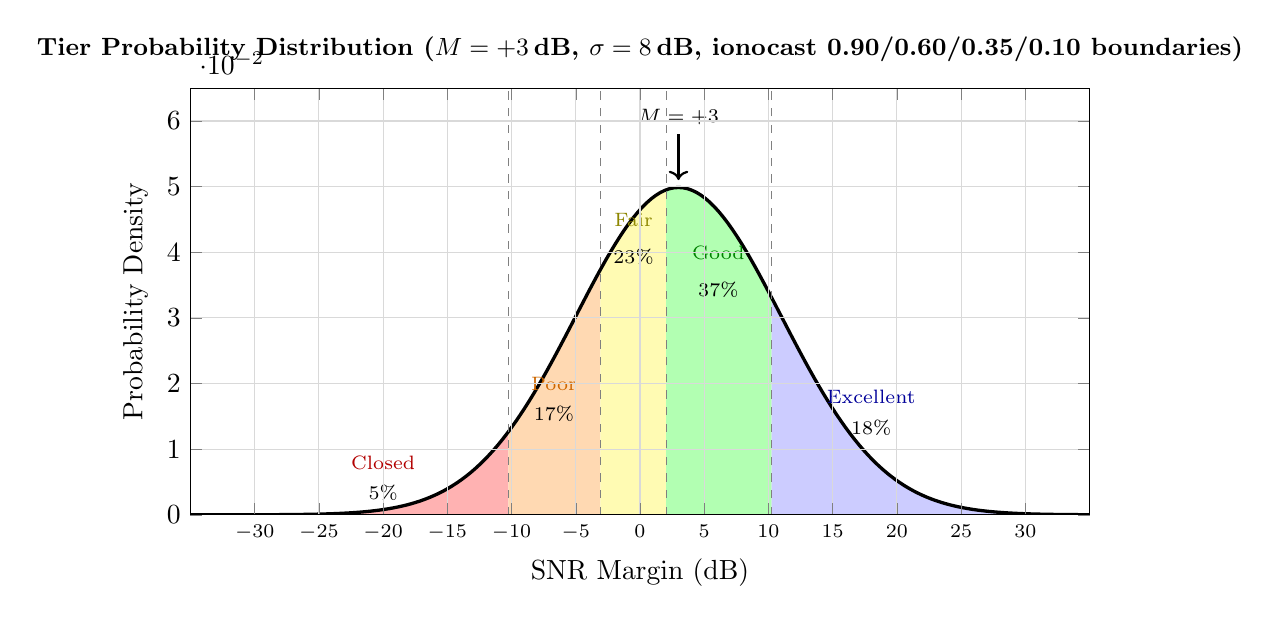
\begin{tikzpicture}
\begin{axis}[
  width=13cm, height=7cm,
  xlabel={SNR Margin (\si{\dB})},
  ylabel={Probability Density},
  xmin=-35, xmax=35,
  ymin=0, ymax=0.065,
  ytick={0,0.01,0.02,0.03,0.04,0.05,0.06},
  xtick={-30,-25,-20,-15,-10,-5,0,5,10,15,20,25,30},
  xticklabel style={font=\scriptsize},
  grid=major,
  grid style={gray!30},
  title={Tier Probability Distribution ($M=+3$\,dB, $\sigma=8$\,dB,
         ionocast 0.90/0.60/0.35/0.10 boundaries)},
  title style={font=\small\bfseries},
  axis on top,
]

% Gaussian PDF, mu=3, sigma=8.
% Post 2026-04-30 second-pass tier boundaries in sigma-units:
%   excellent at +1.2816 sigma = +10.25 dB
%   good      at +0.2533 sigma =  +2.03 dB
%   fair      at -0.3853 sigma =  -3.08 dB
%   poor      at -1.2816 sigma = -10.25 dB
\pgfmathsetmacro{\mmu}{3}
\pgfmathsetmacro{\sig}{8}
\pgfmathsetmacro{\bExc}{1.2816*\sig}       % +10.25
\pgfmathsetmacro{\bGood}{0.2533*\sig}      %  +2.03
\pgfmathsetmacro{\bFair}{-0.3853*\sig}     %  -3.08
\pgfmathsetmacro{\bPoor}{-1.2816*\sig}     % -10.25

\addplot[name path=pdf,black,very thick,domain=-35:35,samples=200]
  {1/(\sig*sqrt(2*pi))*exp(-(x-\mmu)^2/(2*\sig^2))};

\addplot[name path=zero,draw=none,domain=-35:35,samples=2] {0};

% Closed: < -10.25
\addplot[name path=pdfC,draw=none,domain=-35:-10.25,samples=100]
  {1/(\sig*sqrt(2*pi))*exp(-(x-\mmu)^2/(2*\sig^2))};
\addplot[name path=zeroC,draw=none,domain=-35:-10.25,samples=2] {0};
\addplot[red!30] fill between[of=pdfC and zeroC];

% Poor: -10.25 to -3.08
\addplot[name path=pdfP,draw=none,domain=-10.25:-3.08,samples=100]
  {1/(\sig*sqrt(2*pi))*exp(-(x-\mmu)^2/(2*\sig^2))};
\addplot[name path=zeroP,draw=none,domain=-10.25:-3.08,samples=2] {0};
\addplot[orange!30] fill between[of=pdfP and zeroP];

% Fair: -3.08 to +2.03
\addplot[name path=pdfF,draw=none,domain=-3.08:2.03,samples=100]
  {1/(\sig*sqrt(2*pi))*exp(-(x-\mmu)^2/(2*\sig^2))};
\addplot[name path=zeroF,draw=none,domain=-3.08:2.03,samples=2] {0};
\addplot[yellow!30] fill between[of=pdfF and zeroF];

% Good: +2.03 to +10.25
\addplot[name path=pdfG,draw=none,domain=2.03:10.25,samples=100]
  {1/(\sig*sqrt(2*pi))*exp(-(x-\mmu)^2/(2*\sig^2))};
\addplot[name path=zeroG,draw=none,domain=2.03:10.25,samples=2] {0};
\addplot[green!30] fill between[of=pdfG and zeroG];

% Excellent: > +10.25
\addplot[name path=pdfE,draw=none,domain=10.25:35,samples=100]
  {1/(\sig*sqrt(2*pi))*exp(-(x-\mmu)^2/(2*\sig^2))};
\addplot[name path=zeroE,draw=none,domain=10.25:35,samples=2] {0};
\addplot[blue!20] fill between[of=pdfE and zeroE];

% Threshold lines (sigma-relative)
\draw[gray,thin,dashed] (axis cs:-10.25,0) -- (axis cs:-10.25,0.065);
\draw[gray,thin,dashed] (axis cs:-3.08,0)  -- (axis cs:-3.08,0.065);
\draw[gray,thin,dashed] (axis cs:2.03,0)   -- (axis cs:2.03,0.065);
\draw[gray,thin,dashed] (axis cs:10.25,0)  -- (axis cs:10.25,0.065);

% Region labels
\node[font=\scriptsize,red!70!black]    at (axis cs:-20,0.008)  {Closed};
\node[font=\scriptsize,orange!80!black] at (axis cs:-6.7,0.020) {Poor};
\node[font=\scriptsize,olive]           at (axis cs:-0.5,0.045) {Fair};
\node[font=\scriptsize,green!50!black]  at (axis cs:6.1,0.040)  {Good};
\node[font=\scriptsize,blue!60!black]   at (axis cs:18,0.018)   {Excellent};

% Probabilities for M=+3, sigma=8 under post 2026-04-30 boundaries:
%   z_p = (-10.25 - 3) / 8 = -1.6566 ; Phi = 0.0488
%   z_f = ( -3.08 - 3) / 8 = -0.7603 ; Phi = 0.2236
%   z_g = ( +2.03 - 3) / 8 = -0.1218 ; Phi = 0.4515
%   z_e = (+10.25 - 3) / 8 = +0.9066 ; Phi = 0.8177
%   P(Closed)    = 0.0488        ->  5 %
%   P(Poor)      = 0.2236 - 0.0488 = 0.1748 -> 17 %
%   P(Fair)      = 0.4515 - 0.2236 = 0.2279 -> 23 %
%   P(Good)      = 0.8177 - 0.4515 = 0.3662 -> 37 %
%   P(Excellent) = 1 - 0.8177    = 0.1823 -> 18 %
\node[font=\scriptsize,anchor=north] at (axis cs:-20,0.006)  {5\%};
\node[font=\scriptsize,anchor=north] at (axis cs:-6.7,0.018) {17\%};
\node[font=\scriptsize,anchor=north] at (axis cs:-0.5,0.042) {23\%};
\node[font=\scriptsize,anchor=north] at (axis cs:6.1,0.037)  {37\%};
\node[font=\scriptsize,anchor=north] at (axis cs:18,0.016)   {18\%};

% Mean marker
\draw[black,thick,->] (axis cs:3,0.058) -- (axis cs:3,0.0510);
\node[font=\scriptsize,anchor=south] at (axis cs:3,0.058) {$M=+3$};

\end{axis}
\end{tikzpicture}
\caption{Tier probability distribution for a margin of
         $+3$\,dB with $\sigma=8$\,dB under the post 2026-04-30
         second-pass tier boundaries
         (Table~\ref{tab:tiers}). Boundaries are
         $\pm 0.39\sigma / +0.25\sigma$ ($-3.08 / +2.03$\,\si{\dB},
         the Fair band) and $\pm 1.28\sigma$ ($\pm 10.25$\,\si{\dB},
         the Excellent / Closed cutoffs). Most likely tier is Good
         (37\%), with 18\% Excellent and 23\% Fair --- the
         distribution is asymmetric because $M=+3$ sits squarely
         inside Good. The $\sigma = \SI{8}{\dB}$
         shown here is the 6\,m / 2\,m placeholder value
         (Table~\ref{tab:bandsigma}); the HF bands use $\sigma_g
         \in \{6, 10, 12\}$\,dB depending on band.  Read the figure
         as a tier-distribution illustration at an in-between
         $\sigma$ rather than as a representative HF prediction;
         tier widths scale with $\sigma$ and the corresponding
         dB-space boundaries shift accordingly.}
\label{fig:tierprob}
\end{figure}

% ═════════════════════════════════════════════════════════════════════
\section{Tier Mapping}\label{sec:tiers}

Verdicts are computed \emph{per band} (160\,m through 10\,m
individually, plus 6\,m and 2\,m for VHF), not in groups.  For each
band the SNR margin is evaluated on every reference path (short and
long, across all five destinations); the \textbf{best-margin} path
wins and its margin drives the verdict, while the reason string and
\texttt{openDirs} list record which destination that was.  If a single
path is viable, the band is not ``closed'' --- it is open to that
destination, which is material information for the operator.  An
earlier aggregation over the median margin was removed because most
reference paths are long transcontinental hops that are routinely
over-MUF or night-crossing; the median was dominated by failing paths
and buried genuinely open short paths (e.g.\ a 944\,km EM79--NYC path
reporting \SI{+27}{\dB} margin would have its verdict overwritten by
the median of eight failing long paths).

\paragraph{Best-path summary, full-detail companion.}  The
band-table row shows the best-margin destination only (the
``Best Path'' column), which is a deliberate compression:
displaying all ten path columns per row would be visually
unworkable on small screens.  An operator who wants the
underlying per-destination breakdown consults the Reference
Paths panel in the Ionosphere section, which lists the kc2g MUF
on each of the 10 paths with a colour-coded f/MUF column for
the band currently selected.  The two surfaces share the same
underlying budget; the band-table row is the headline, the
Reference Paths panel is the source-of-truth.  The Best-Path
column itself is therefore only a hint --- if it reads
``Tokyo'' on 20\,m and the operator wants Argentina, the
Reference Paths panel is what to consult next.

The continuous margin is discretised into five operator-facing tiers
defined as ITU-R P.842 \cite{itup842} circuit-reliability buckets
(Table~\ref{tab:tiers}).  Each tier corresponds to a fixed
reliability $R = \Phi(M/\sigma)$ rather than a fixed dB margin, so
the boundaries scale with each band's prediction uncertainty
$\sigma_g$ (Section~\ref{sec:reliability}).  The tier label answers
``how often will a QSO complete on this band right now, with the
station the operator has configured?'' --- and is therefore a
property of the user's actual rig, not of an abstract reference
station.  The defaults (100\,W SSB, 5\,dBi horizontal dipole,
suburban noise) match the canonical first-visit operator profile;
any change to power, mode, antenna, or noise environment recomputes
the SNR budget and reshapes the verdict accordingly.

Earlier versions of ionocast hand-set the dB boundaries
($+18 / +6 / -5 / -14$) and validated the tiers against per-band
WSPR-spot percentiles \cite{wsprlive}.  That validation target was
replaced because WSPR-spot activity measures who is transmitting,
not whether a QSO would complete on the configured station.  Tier
verdicts are now defined entirely by the SNR budget plus
Equation~\ref{eq:reliability}; the harness retains a binary
``$\geq 50$ spots/h'' activity check as a sanity floor only.

\begin{table}[H]
\centering
\caption{Tier thresholds, expressed as ITU-R P.842 circuit-reliability
buckets.  $R$ is computed by Equation~\ref{eq:reliability}; the
margin column is the corresponding boundary in $\sigma$-units.
The actual boundary in dB is band-specific via the per-band
$\sigma_g$ from Table~\ref{tab:bandsigma}: lower-mid HF bands
($\sigma_g = \SI{8}{\dB}$ on 160m--40m, $\SI{9}{\dB}$ on 30m / 20m / 17m
post 2026-04-30 $\sigma$ refit) put ``excellent'' at $\approx +10$--$12\,\si{\dB}$
and ``good'' at $\approx +2.0$--$2.3\,\si{\dB}$; the upper HF bands
(15m at $\sigma_g = \SI{10}{\dB}$, 12m / 10m at $\SI{12}{\dB}$) at
$\approx +12.8$--$15.4 / +2.5$--$3.0\,\si{\dB}$.  The boundaries are
symmetric: Excellent at $+1.2816\,\sigma$ ($R \ge 90\%$) and Closed at
$-1.2816\,\sigma$ ($R < 10\%$) are mirror images.}
\label{tab:tiers}
\begin{tabular}{@{}llll@{}}
\toprule
\textbf{Tier} & \textbf{Reliability} & \textbf{Margin (in $\sigma$)} & \textbf{Meaning} \\
\midrule
Excellent & {$R \geq 90\%$} & {$\geq +1.2816\,\sigma$} & QSO completes $\approx 9$ of 10 attempts \\
Good      & {$R \geq 60\%$} & {$\geq +0.2533\,\sigma$} & Comfortable contacts; 3 of 5 attempts \\
Fair      & {$R \geq 35\%$} & {$\geq -0.3853\,\sigma$} & Marginal; FT8/WSPR reliable, SSB iffy \\
Poor      & {$R \geq 10\%$} & {$\geq -1.2816\,\sigma$} & Long shot; only digital modes likely \\
Closed    & {$R <  10\%$}   & {$< -1.2816\,\sigma$}    & Band effectively closed \\
\bottomrule
\end{tabular}
\end{table}

\paragraph{Threshold history (2026-04-28 / 2026-04-30).}
The first cut (2026-04-28) used the classical P.842 boundaries at
$\pm 0.8416\,\sigma$ and $\pm 1.6449\,\sigma$ ($R = 0.95 / 0.80 /
0.50 / 0.20$), which align cleanly with the standard but were
calibrated for $\sigma_g = \SI{6}{\dB}$.  The 2026-04-30 $\sigma$
refit raised lower-mid-band $\sigma_g$ to \SI{8}--\SI{9}{\dB},
making the old Good threshold ($\geq +6.7\,\si{\dB}$ at $\sigma =
8$) hard to clear: most upper-band paths landed in Fair,
producing a visually flat tier distribution.  A first loosening
that day pulled the boundaries to $0.95 / 0.62 / 0.35 / 0.12$,
but kept Excellent strict at $\geq +1.6449\,\sigma$ (still $\sim
\SI{13}{\dB}$ on lower-mid bands, rarely reachable) and the Good
$z$-value of $0.31$ was a too-precise number chosen to clear one
specific 20m path.  A second pass the same day re-anchored the
thresholds to the operator's failure-rate intuition: Excellent
$\approx 1$ in 10 fail, Good $\approx 4$ in 10 fail, Fair the
coin-flip-down band, Poor $\approx 9$ in 10 fail, Closed
essentially always.  That is the $0.90 / 0.60 / 0.35 / 0.10$
schedule shown above, with Excellent / Closed boundaries
symmetric at $\pm 1.2816\,\sigma$.  Excellent at $\sigma_g =
\SI{9}{\dB}$ now sits at $\sim \SI{11.5}{\dB}$ which is reachable
on a strong DX path; Good at $+0.2533\,\sigma \approx
\SI{2.3}{\dB}$ clears comfortably with a few-dB margin.  An
unconditional $\sigma_g = \SI{8}{\dB}$ fallback exists in
\texttt{tier.js} as \texttt{DEFAULT\_SIGMA\_DB}.

\subsection{WSPR Activity Override}\label{sec:spot-override}

WSPR spot counts give an independent observational signal that the
physics budget does not consume directly.  When observed activity for
a band exceeds 1.3$\times$ the band's 30-day mean for the current
UTC hour \emph{and} the physics-derived tier is currently below
``Good'' (i.e., Fair, Poor, or Closed), the verdict is promoted to
Good.  This catches openings outside the budget --- weak
sporadic-E, off-axis scatter, propagation modes that the
climatology underweights.

The override is a strict one-way ratchet \emph{capped at Good as a
promotion ceiling, not a global ceiling}: a physics-Excellent
verdict is preserved (the tier-rank condition is false when the
prior tier is already at or above Good, so the override never
fires); a physics-Fair verdict can be promoted to Good but no
higher; physics-Poor and physics-Closed can also only be promoted
to Good. Low or absent activity does not invalidate the physics;
it might just mean nobody is on the air, so the override never
demotes.

\paragraph{Where the override appears in the UI.}  Two surfaces
display per-band conditions and they handle the override
differently --- by design, to avoid pathologies where the row tier
and the row Stability percent appear to disagree:
\begin{itemize}[nosep]
  \item \textbf{Per-band table rows} (HF Bands panel): the Tier
        column and the Stability column both come from the
        physics-derived $M, \sigma$ via
        \texttt{bestPerBand[name].tier} and
        \texttt{bestPerBand[name].stability}.  The override does
        \emph{not} enter individual rows.  Tier and Stability are
        therefore internally consistent within each row: a centred
        physics-Fair row reads ``Fair'' near the 66\,\% middle-tier
        ceiling; a tail-deep physics-Excellent row reads
        ``Excellent'' near 100\,\%.
  \item \textbf{Band-group summary line} (e.g., ``20\,m: Good ·
        margin 5\,dB · unusually active: 100 spots/h vs avg 30''):
        the Tier comes from the override-promoted value when the
        override fires.  In that case, the Stability percent is
        \emph{suppressed} from the line and replaced by the
        activity note --- the operator sees \emph{why} the group
        was promoted rather than a numerically inconsistent
        Stability computed against the wrong tier bucket.
\end{itemize}
The architecture deliberately splits per-band detail (physics
truth) from group-level summary (override-aware) so neither
display ever forces the operator to read ``Good · 27\,\%''.

\paragraph{Data-driven baselines.}  The reference is the
30-day \emph{mean} hourly spot count per (band, UTC-hour),
regenerated daily by the \texttt{wspr-baselines.yml} GitHub
Actions workflow (a 06:00 UTC cron job that runs
\texttt{node scripts/harness.mjs wspr-baselines} and commits the
diff to \texttt{src/data/spot-baselines.mjs}, providing a true
sliding 30-day window that tracks solar-cycle progression and
seasonal shifts without manual intervention):

\begin{quote}\small\ttfamily
SELECT band, hour\_utc, sum(hourly\_count) / 30.0 AS avg\\
FROM (\\
\phantom{x}SELECT band, toStartOfHour(time) AS h,\\
\phantom{xSELECT }toHour(time) AS hour\_utc,\\
\phantom{xSELECT }count() AS hourly\_count\\
\phantom{x}FROM wspr.rx\\
\phantom{x}WHERE time >= now() - INTERVAL 30 DAY\\
\phantom{x}GROUP BY band, h, hour\_utc\\
) GROUP BY band, hour\_utc
\end{quote}

The outer aggregator divides total spots in the (band, hour) cell
by the window length in days rather than averaging over only the
hours that had at least one spot.  Earlier code used \texttt{avg
(hourly\_count)}, which silently skipped (band, hour) cells with
zero spots in a given day --- ClickHouse \texttt{GROUP BY} doesn't
emit a row for an empty group --- so the 30-day mean on quiet
cells (e.g.\ 10\,m at 03 UTC during low-cycle phase) was the
average over the days the band was actually open, not the average
over all 30 days.  The inner \texttt{GROUP BY band, h, hour\_utc}
groups by both \texttt{toStartOfHour(time)} (full date+hour
timestamp) and \texttt{toHour(time)} (hour-of-day in [0, 23]); the
two carry partially-redundant information but the redundancy is
intentional: \texttt{h} drives the per-day-per-hour
\texttt{hourly\_count}, and \texttt{hour\_utc} is what the outer
group then averages over to collapse the 30-day window into a
24-hour cycle.  Dropping either column would lose one of those
two roles.  The over-counted baseline raised the override
threshold on exactly the cells where the override most needs to
fire on rare openings.  Dividing by the literal day count fixes
that.

This produces a $10 \times 24$ matrix of typical hourly spot rates
across all days of the week.  The override fires when observed
activity exceeds $1.3 \times$ the matrix entry for the current
(band, UTC-hour) cell --- ``the band is \emph{meaningfully}
busier than usual for this time of day.''  An earlier formulation
used a Mon--Fri-only baseline (\,\texttt{toDayOfWeek(time) < 6}\,)
as a cheap contest-weekend filter, but that biased the comparison:
the live observation includes weekends, so on Saturday the
override compared current spots against a weekday-only mean and
fired far too easily on routine weekend operating activity.
Including weekends in the rolling baseline restores the
like-for-like comparison; major contest weekends are $<\!10\,\%$
of weeks in a 30-day window so their inflation of the mean is
bounded, and they affect the override ratio in both directions
(a current contest day reads proportionally less anomalous
against a slightly inflated mean).  WSPR
hourly spot counts are over-dispersed Poisson with strong diurnal
structure and a coefficient of variation that ranges from
${\sim}0.3$ on heavily-trafficked daytime cells (20\,m at 1500\,UTC)
to ${\sim}1.5$ on quiet upper-band predawn cells (10\,m at
0300\,UTC), so the $1.3\times$ threshold corresponds to anywhere
between mean\,+\,$1\sigma$ and mean\,+\,$0.2\sigma$ depending on
band and hour.  Tightening to a bare $\text{spots} > \text{mean}$
comparison would fire on every above-median hour and over-promote
borderline cases; the multiplier was empirically chosen as the
smallest value that filters out routine above-average hours
without missing genuinely anomalous activity.  The choice was
made by sweeping candidate thresholds in $\{1.0, 1.1, \ldots, 2.0\}$
against the same 30-day WSPR baseline data used to construct the
matrix (\texttt{wspr.rx} table, 2026-04 window): 1.3$\times$ was
the smallest ratio at which the override fired on roughly 5--10\%
of (band, hour) cells per day --- low enough to read as
``unusual'' rather than ``daily routine'', high enough to keep
the override actionable on the cells where it matters (off-axis
sporadic-E days, evening 15\,m enhancement during HSS recovery,
the ${\sim}5$\,\% of 10\,m cells where 30-day-mean is near zero
but live counts climb to tens).  Combined with the Good promotion
ceiling, the threshold keeps the override an ``unusually active''
signal across all (band, hour) cells.

The baseline matrix is emitted as a plain ES module at
\texttt{src/data/spot-baselines.mjs} and imported at runtime by the
derive pipeline.  It is currently re-generated manually every few
months, which is too slow at solar-cycle phase transitions where
band-activity patterns can drift on weeks (cycle-25 ascending phase
saw 30\,m and 17\,m baselines climb measurably month-over-month
through 2024).  The point-in-time regeneration cadence is a
maintenance artefact rather than a calibrated cadence: a sliding
30-day baseline updated daily would track activity changes
properly without retraining the harness, at the cost of one
ClickHouse query per day to refresh the matrix.  The shipped form
is versioned with the rest of the codebase so fresh checkouts ship
with valid baselines out of the box; switching to the daily-sliding
form is candidate operational work tracked in
Section~\ref{sec:limits}.

\paragraph{Reception-population bias in the baseline.}  The
\texttt{wspr.rx} aggregate counts spots received by listening
stations.  WSPR receivers are heavily concentrated in North America
and Europe (operator-population statistics from
\texttt{wsprnet.org}'s active-stations roster; ${\sim}60\%$ of
worldwide WSPR receivers sit in those two regions, with another
${\sim}15\%$ in the AU/NZ/JA cluster), so a 30-day baseline of
``${\sim}100$ spots/h on 20\,m at 0900\,UTC'' reflects predominantly
North American daytime listening rather than a globally-uniform
``activity at this hour''.  The override fires uniformly across the
operator population, but the activation threshold reflects
NA/EU/Pacific listening windows.  Operators outside those regions
(AF, low-income tropical-belt countries, Central Asia) see a
baseline whose 24-hour shape is set by other regions' UTC clocks
rather than by their local-time activity rhythm; the override
correctly fires when the global aggregate runs hot, but the
``unusually active for this hour'' interpretation holds most
crisply in the receiver-dense regions.  A per-region renormalisation
is candidate work, gated on enough per-pair receiver coverage to
fit regional baselines without over-fitting noise.

% ═════════════════════════════════════════════════════════════════════
% ── Additional Figures ───────────────────────────────────────────────

% ── Noise power-sum figure ───────────────────────────────────────────
\begin{figure}[H]
\centering
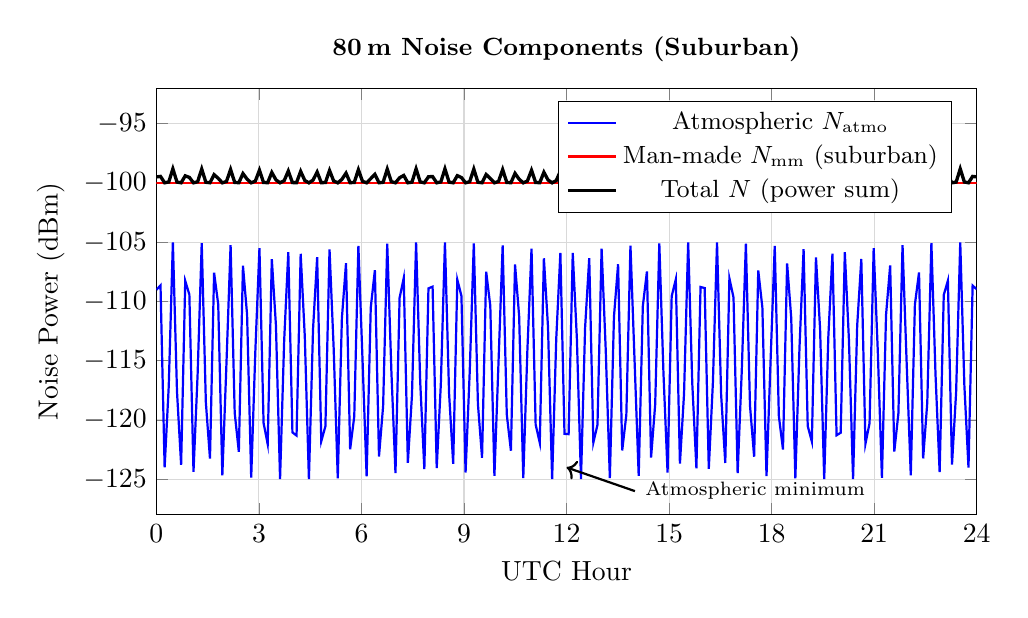
\begin{tikzpicture}
\begin{axis}[
  width=12cm, height=7cm,
  xlabel={UTC Hour},
  ylabel={Noise Power (\si{\dBm})},
  xmin=0, xmax=24,
  ymin=-128, ymax=-92,
  xtick={0,3,6,9,12,15,18,21,24},
  ytick={-125,-120,-115,-110,-105,-100,-95},
  grid=major,
  grid style={gray!30},
  legend pos=north east,
  legend style={font=\small},
  title={80\,m Noise Components (Suburban)},
  title style={font=\small\bfseries},
]

% 80m: Nbase = -115
% Atmospheric: Natmo = -115 + (-10 * cos(chi))
% At midnight cos(chi) ≈ -1 → Natmo = -115 + 10 = -105
% At noon cos(chi) ≈ 1 → Natmo = -115 - 10 = -125
% Using cos(chi) ≈ cos((x-12)*pi/12) for simple diurnal

\addplot[blue,thick,domain=0:24,samples=200]
  {-115 + (-10)*cos(deg((x-12)/12*180))};
\addlegendentry{Atmospheric $N_{\text{atmo}}$}

% Man-made: Nmm = -115 + 15 = -100 (flat)
\addplot[red,thick,domain=0:24,samples=2]
  {-100};
\addlegendentry{Man-made $N_{\text{mm}}$ (suburban)}

% Total: power sum
% N = 10*log10(10^(Natmo/10) + 10^(-100/10))
\addplot[black,very thick,domain=0:24,samples=200]
  {10*log10(10^((-115 + (-10)*cos(deg((x-12)/12*180)))/10) + 10^(-100/10))};
\addlegendentry{Total $N$ (power sum)}

% Annotation
\draw[<-,thick] (axis cs:12,-124) -- (axis cs:14,-126)
  node[anchor=west,font=\scriptsize] {Atmospheric minimum};
\draw[<-,thick] (axis cs:12,-100) -- (axis cs:14.5,-97)
  node[anchor=west,font=\scriptsize] {Man-made dominates};

\end{axis}
\end{tikzpicture}
\caption{Noise power components on 80\,m in a suburban environment.
         The man-made noise (\SI{-100}{\dBm}) dominates at all hours;
         the atmospheric diurnal swing barely affects the total.  This
         power-sum model prevents the phantom \SI{7}{\dB} margin that
         a linear (dB-domain) sum would produce at midday.}
\label{fig:noise}
\end{figure}

% ── D-region absorption by band ──────────────────────────────────────
\begin{figure}[H]
\centering
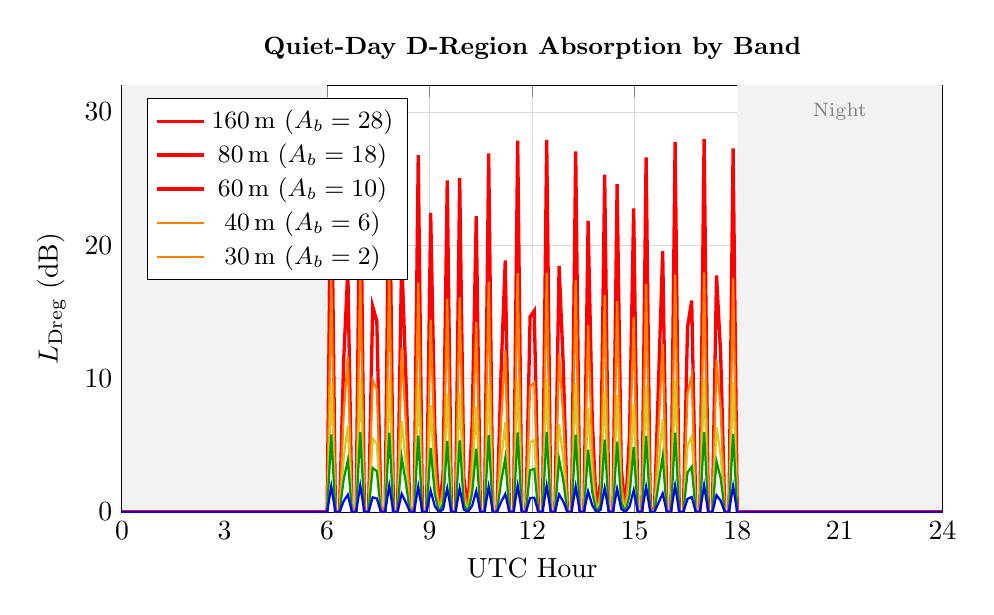
\begin{tikzpicture}
\begin{axis}[
  width=12cm, height=7cm,
  xlabel={UTC Hour},
  ylabel={$L_{\text{Dreg}}$ (\si{\dB})},
  xmin=0, xmax=24,
  ymin=0, ymax=32,
  xtick={0,3,6,9,12,15,18,21,24},
  grid=major,
  grid style={gray!30},
  legend pos=north west,
  legend style={font=\small},
  title={Quiet-Day D-Region Absorption by Band},
  title style={font=\small\bfseries},
]

% cos(chi) ≈ max(0, cos((x-12)*pi/12))
% LabsD = Abase * max(0, cos(chi))^1.3
% Night: cos(chi) < 0.05 → 0

% 160m: Abase = 28
\addplot[red,very thick,domain=6:18,samples=100]
  {28 * (max(0, cos(deg((x-12)/12*180))))^1.3};
\addplot[red,very thick,domain=0:6,samples=20] {0};
\addplot[red,very thick,domain=18:24,samples=20] {0};
\addlegendentry{160\,m ($A_b=28$)}

% 80m: Abase = 18
\addplot[orange,thick,domain=6:18,samples=100]
  {18 * (max(0, cos(deg((x-12)/12*180))))^1.3};
\addplot[orange,thick,domain=0:6,samples=20] {0};
\addplot[orange,thick,domain=18:24,samples=20] {0};
\addlegendentry{80\,m ($A_b=18$)}

% 60m: Abase = 10
\addplot[yellow!80!black,thick,domain=6:18,samples=100]
  {10 * (max(0, cos(deg((x-12)/12*180))))^1.3};
\addplot[yellow!80!black,thick,domain=0:6,samples=20] {0};
\addplot[yellow!80!black,thick,domain=18:24,samples=20] {0};
\addlegendentry{60\,m ($A_b=10$)}

% 40m: Abase = 6
\addplot[green!60!black,thick,domain=6:18,samples=100]
  {6 * (max(0, cos(deg((x-12)/12*180))))^1.3};
\addplot[green!60!black,thick,domain=0:6,samples=20] {0};
\addplot[green!60!black,thick,domain=18:24,samples=20] {0};
\addlegendentry{40\,m ($A_b=6$)}

% 30m: Abase = 2
\addplot[blue,thick,domain=6:18,samples=100]
  {2 * (max(0, cos(deg((x-12)/12*180))))^1.3};
\addplot[blue,thick,domain=0:6,samples=20] {0};
\addplot[blue,thick,domain=18:24,samples=20] {0};
\addlegendentry{30\,m ($A_b=2$)}

% Night shading
\addplot[name path=top,draw=none,domain=0:6,samples=2] {32};
\addplot[name path=bot,draw=none,domain=0:6,samples=2] {0};
\addplot[gray!10] fill between[of=top and bot];
\addplot[name path=top2,draw=none,domain=18:24,samples=2] {32};
\addplot[name path=bot2,draw=none,domain=18:24,samples=2] {0};
\addplot[gray!10] fill between[of=top2 and bot2];

\node[font=\scriptsize,gray] at (axis cs:3,30) {Night};
\node[font=\scriptsize,gray] at (axis cs:21,30) {Night};

\end{axis}
\end{tikzpicture}
\caption{Quiet-day D-region absorption by band.  160\,m reaches
         \SI{28}{\dB} at local noon; 30\,m and above are essentially
         unaffected.  Night absorption is zero.  The illustrative
         curves show a smooth descent toward zero at low
         $\cos\chi$, but the actual implementation hard-gates
         $L_{\text{Dreg}} = 0$ at $\cos\chi < 0.05$
         (Eq.~\ref{eq:labsd}); the figure smooths that gate for
         readability rather than showing the cliff.}
\label{fig:dabs}
\end{figure}

% ═════════════════════════════════════════════════════════════════════
\section{Output Formatting and Alerts}\label{sec:output}

The tiers and indices produced by the foregoing pipeline are
surfaced across an eight-panel web UI:

\begin{itemize}[nosep]
  \item \textbf{Active Alerts} (\S\ref{sec:alerts}): SWPC-bulletin
        feed plus rule-derived ``soft'' alerts in one
        severity-sorted list at the top of the page.
  \item \textbf{HF Bands}: the ten HF amateur bands as a per-band
        table.  Each row shows the band frequency, the predicted
        verdict tier (Excellent / Good / Fair / Poor / Closed
        per Section~\ref{sec:tiers}), the SNR margin in dB, the
        Stability percent
        (Eq.~\ref{eq:tierstab}: $\Phi$ of $\sigma$-distance to the
        nearest tier boundary; bucket-width-independent and so
        directly readable on an absolute scale --- 50\,\% at a
        boundary, ${\sim}84$\,\% one $\sigma$ inside, $\to 100$\,\%
        deep inside), the dominant propagation mode (F2 / NVIS /
        Es / Aurora), and the best-margin destination from the
        path basket.  Distinct from circuit reliability $R$ of
        Eq.~\ref{eq:reliability}: $R$ is the probability the link
        is viable, Stability is the probability the verdict
        \emph{label} is robust to within-$\sigma$ noise.  The
        ``Best Path'' cell is a compression of the underlying
        10-path evaluation; for the per-destination breakdown
        consult the Reference Paths sub-panel in the Ionosphere
        section (cross-referenced by the cell's info popover).
  \item \textbf{VHF Bands}: 6\,m and 2\,m mirrored from the HF
        layout, with Es-MUF / aurora / meteor-scatter mode
        labelling instead of F2.  A second panel below the band
        table renders per-station tropospheric ducting status from
        the 24-station UWyo radiosonde basket
        (Section~\ref{sec:tropo}): each row shows the lowest-1\,km
        $\mathrm{d}N/\mathrm{d}h$ and an ITU-R P.453 classification
        (standard / super-refractive / ducting), sorted ducting
        first so an active event surfaces at the top.
  \item \textbf{Upcoming Disruptions} (outlook): SWPC's 3-day
        R/S/G probability table, the SWPC 3-h $K_p$ forecast,
        Earth-directed CMEs from NASA DONKI, IMO-catalogue meteor
        showers, top active solar regions, and the 27-day
        ISES SFI / $A_p$ outlook.
  \item \textbf{Ionosphere}: nearest-GIRO-station digisonde
        readings (foF2 / foEs / hmF2), GNSS TEC, 30\,MHz cosmic
        noise, the Reference Paths panel --- the per-QTH path
        table listing kc2g MUF on the five short-path destinations
        and their long-path counterparts, ten paths total ---
        plus the kc2g global foF2 map and the GloTEC TEC map.
        The Reference Paths panel is the source-of-truth that
        Section~\ref{sec:tiers}'s band-table Best-Path column
        compresses; an operator who wants per-destination detail
        rather than the headline winner consults this panel.
  \item \textbf{Geomagnetic}: $K_p$ / $A_p$ / $D_{\text{st}}$ /
        $H_{p30}$ / Sym-H / AE / aurora HP indices, a 7-day
        $K_p$ trend chart, and the OVATION aurora forecast and
        D-RAP map.
  \item \textbf{Solar}: SFI / SN / X-ray class / proton flux
        indices, real-time DSCOVR / ACE solar wind ($B_z$ /
        $V_{sw}$ / $n$), and SDO imagery (\,EUV~193 / EUV~304 /
        magnetogram\,).
  \item \textbf{Links}: data source attribution, license credits,
        and links to the upstream services.
\end{itemize}

This section documents the assembly logic for the two surfaces
that depend on derived numeric thresholds (the alerts panel
soft-rule grader, and the per-band tier verdict feeding the HF /
VHF tables); the layout choices for the other panels are
data-source documentation rather than algorithm.

\subsection{Algorithmic surfaces and data-source surfaces}

Of the eight panels above, three have non-trivial assembly logic
that this section documents:
\begin{itemize}[nosep]
  \item \emph{Active Alerts} (\S\ref{sec:alerts}, below) combines
        SWPC bulletins with rule-derived ``soft'' alerts whose
        thresholds are model-side numeric constants rather than
        upstream fields.
  \item the \emph{HF Bands} and \emph{VHF Bands} tables surface
        per-band $(M, \sigma) \to$ tier verdicts already
        documented in detail in Sections~\ref{sec:snr},
        \ref{sec:reliability}, and \ref{sec:tiers}; their layout
        is just a transposition of those into table rows.
  \item the \emph{Reference Paths} sub-panel (inside the
        Ionosphere panel) computes per-QTH great-circle midpoints
        for five canonical destinations and their long-path
        counterparts (10 paths total), looks up the nearest
        kc2g ionosonde for each midpoint subject to a
        \SI{30}{\minute} freshness gate, and renders the
        per-path MUF with a colour-coded f/MUF column for the
        band currently selected by the band table.  This is the
        full-detail companion to the band table's compressed
        Best Path column (Section~\ref{sec:tiers}).
\end{itemize}
The remaining five panels (Upcoming Disruptions, the rest of
Ionosphere outside Reference Paths, Geomagnetic, Solar, Links)
are data-source documentation: each block
is a labelled rendering of a fetched upstream (SWPC / DONKI / IMO
/ kc2g / GIRO / SDO) without ionocast-side processing.  Their
assembly logic lives in the data fetchers and the
\texttt{src/ui/sections.js} layout description rather than in
this section; an operator-facing description of each block sits
inline in the panel's \texttt{interp} attribute and is displayed
when the panel's info badge is clicked.

\paragraph{Reading the Stability column at a glance.}  The
band-table column displays $S(M, \sigma)$ from
Eq.~\ref{eq:tierstab}: $\Phi$ of the $\sigma$-distance to the
nearest tier boundary.  Bucket-width-independent, so a centred
Fair verdict and a centred Excellent verdict at the same
$\sigma$-offset from their respective nearest boundaries read the
same percentage.  Operator reading: 50\,\% at the boundary itself,
${\sim}84$\,\% one $\sigma$ inside the bucket, asymptotic to
100\,\% deep inside; finite-width middle buckets (Poor / Fair /
Good) cap at $\Phi(0.42) \approx 66\,\%$ at the bucket centre, so
read mid-tier values relative to the 66\,\% centred ceiling and
open-ended Closed / Excellent values against the absolute scale.
The earlier band-table column displayed the two-sided literal
$P(\text{predicted}=\text{true})$ form $C(M, \sigma)$, which
capped at $\sim 32\,\%$ on centred middle tiers and required a
``(peak)'' annotation to stay readable; that column was retired
in 2026-04 in favour of $S$, which the production UI
(\texttt{src/ui/builders/tables.js}) now surfaces directly.

\subsection{Active Alerts Panel}\label{sec:alerts}

The alerts panel combines two rendering pipelines into one
severity-sorted list.

\paragraph{Official SWPC feed.}  A polling fetch of
\texttt{products/alerts.json} emits up to four recent items.
Each item's severity level is derived from its
\texttt{product\_id} by regex: matches on \texttt{ALERT} or
\texttt{WARNING} render as \emph{alert}, \texttt{WATCH} as
\emph{watch}, \texttt{SUMMARY} or \texttt{FORECAST} as
\emph{info}; the fallback is \emph{warn}.

\paragraph{Rule-derived (soft) alerts.}  Eight rules run on every
refresh against the same data bundle the per-band budget consumes
($K_p$, $B_z$, $D_{\text{st}}$, aurora HP, DRAP, GOES X-ray, GOES
$\ge 10$\,MeV protons, and storm-lag effective $K_p$).
Each rule is \emph{graded} and short-circuits at the highest
matching tier, so $K_p = 9$ does not simultaneously fire G5,
G4, G3, G2, and G1.  Thresholds reuse the constants documented
in Sections~\ref{sec:snr}--\ref{sec:projection}; no new magic
numbers are introduced.

\paragraph{Intra-tier sort order.}  Alerts are sorted primarily
by severity tier (\emph{alert} > \emph{watch} > \emph{warn} >
\emph{info}); within a single tier the rule iteration order is
the deterministic tiebreak: FLARE first (most time-urgent ---
X-ray ionisation peaks within seconds of the flare event,
operator response window is minutes), then geomagnetic indices
($K_p$, $B_z$, $D_{\text{st}}$ in that order, reflecting the
upstream causal chain --- $B_z$ at the L1 monitor leads
geomagnetic-effect $K_p$ at Earth by $\sim$30--60\,min via
solar-wind transit \SI{1.5e6}{\km}/$v_{\text{sw}}$, and $K_p$
leads $D_{\text{st}}$ by $\sim$30--60\,min via ring-current
buildup time; the L1-to-Earth lead is the larger and more
operationally useful of the two), then aurora, DRAP, PCA, and storm
recovery.  The fixed order means repeated refreshes show the
same chip arrangement, so an operator scanning the panel
between refreshes can pattern-match position rather than
re-read each line.

\begin{table}[H]
\centering
\caption{Soft-alert rule set.  Severity maps to the same
         \emph{info / warn / watch / alert} levels used by the
         SWPC renderer; \emph{alert} ranks highest.}
\label{tab:soft-alerts}
\begin{tabular}{@{}l l l l@{}}
\toprule
\textbf{Trigger} & \textbf{Threshold} & \textbf{Level} & \textbf{Label} \\
\midrule
X-ray flare                  & class $\ge$ M5          & alert & FLARE \\
                             & class $\in$ M1--M4.9    & watch & FLARE \\
\midrule
Geomagnetic $K_p$            & $K_p \ge 9$             & alert & G5 \\
                             & $K_p \ge 8$             & alert & G4 \\
                             & $K_p \ge 7$             & alert & G3 \\
                             & $K_p \ge 6$             & alert & G2 \\
                             & $K_p \ge 5$             & watch & G1 \\
\midrule
IMF $B_z$ southward          & $B_z \le -10$\,nT       & alert & BZ SOUTH \\
                             & $B_z \le -5$\,nT        & watch & BZ SOUTH \\
\midrule
Ring current $D_{\text{st}}$ & $D_{\text{st}} \le -150$\,nT & alert & DST SEVERE \\
                             & $D_{\text{st}} \le -100$\,nT & alert & DST STRONG \\
                             & $D_{\text{st}} \le -50$\,nT  & watch & DST MODERATE \\
\midrule
Aurora HP                    & HP $\ge \SI{100}{\GW}$  & watch & AURORA \\
                             & HP $\ge \SI{50}{\GW}$   & info  & AURORA \\
\midrule
D-region absorption at QTH   & DRAP $\ge \SI{10}{\MHz}$ & alert & ABSORPTION \\
                             & DRAP $\ge \SI{5}{\MHz}$  & watch & ABSORPTION \\
\midrule
Polar cap absorption         & flux $\ge 1000$\,pfu & alert & PCA S3 \\
                             & flux $\ge 100$\,pfu  & alert & PCA S2 \\
                             & flux $\ge 10$\,pfu   & watch & PCA S1 \\
\midrule
Storm recovery tail          & $K_{p,\text{eff}} - K_p \ge 1$ \& $K_{p,\text{eff}} \ge 4$ & info & STORM TAIL \\
\bottomrule
\end{tabular}
\end{table}

Soft alerts render alongside SWPC notices rather than only when
the official feed is empty: the derived context --- southward
$B_z$, falling $D_{\text{st}}$, DRAP blanketing QTH --- is
material information SWPC does not publish until formal watch
or warning bulletins are issued, which may lag the underlying
event by several hours.

% ═════════════════════════════════════════════════════════════════════
\section{Known Limitations and Future Work}\label{sec:limits}

The items below are the model's currently-known shortcomings and
the cleanups they imply.  They mix three classes that a reader
prioritising follow-up work may want to disentangle:
\emph{physics gaps} where the model omits a propagation mechanism
or approximates one (\#2 TX pattern, \#3 NVIS height, \#4 RX-side
noise rejection, \#5--\#7 anomalies and SID decay, \#10--\#11
equatorial / polar residuals, \#13 Es coverage, \#14
$N_{\text{base}}$ residual);
\emph{validation gaps} where the metric or the calibration target
has a known ceiling (\#9 binary-accuracy ceiling, \#12
$w_{\text{sc}}$ tied to a metric with a structural cap);
and \emph{process / calibration cadence} items where the
infrastructure rather than the physics is the bottleneck
(\#1 in-app feedback warm-up, \#8 upper-band scatter-recovery
dependence as an implementation status note).  The numbering is
chronological by when the item entered the backlog.

\begin{enumerate}[leftmargin=*]
  \item \textbf{Per-user bias correction needs 2--4 weeks of in-app
        feedback to converge.}  The on-device validation feedback loop
        (Section~\ref{sec:ensemble}) tightens per-band bias and
        $\sigma$ as the operator scores predictions; until at least
        ten samples accumulate per (band, forecast-horizon) cell the
        correction defaults to zero and $\sigma$ to the per-band
        base from Table~\ref{tab:bandsigma} (\SI{6}{\dB} on
        160\,m--20\,m, \SI{10}{\dB} on 17\,m, \SI{12}{\dB} on
        15\,m / 12\,m / 10\,m, \SI{8}{\dB} on the VHF placeholders;
        the unconditional \SI{8}{\dB} fallback is reached only when
        the band-frequency lookup misses entirely, which the BANDS
        table makes impossible in production).  This is independent
        of the offline harness (Section~\ref{sec:calibrate}), which
        already validates the global tune against 30~d of WSPR
        aggregates.

  \item \textbf{TX antenna pattern is an elevation-only cut.}
        The type + height + $\lambda$ model (Section~\ref{sec:antpattern})
        captures the dominant TX-side physics -- ground-reflection
        lobe position, free-space directivity, and polarisation --
        but misses second-order effects on the transmit budget:
        azimuth is not modelled (we don't know where a beam is
        pointed, so beams get their elevation-cut gain only);
        ground conductivity is fixed at ``average soil'' for all
        verticals (salt-water / sea-shore verticals are
        ${\sim}\SI{3}{\dB}$ better); the real-earth pseudo-Brewster
        null on verticals (${\sim}5$--$\SI{8}{\dB}$ dip around
        $3$--$8\degree$ elevation over average soil) is absent;
        and beams are treated as having the same elevation-lobe
        shape as a horizontal wire at the same height, which is
        correct for the main lobe but misses the additional
        off-broadside suppression a multi-element array provides.

  \item \textbf{NVIS model uses foF2 directly.}  For paths
        $<$\,\SI{500}{\km} the model substitutes GIRO foF2 as the
        effective MUF.  A more accurate NVIS model would account for
        layer height and off-vertical angles up to $\sim$\SI{70}{\degree}.

  \item \textbf{No receive-side directional noise rejection.}  A
        physically distinct effect from \#2 above: the
        transmit-side pattern affects the radiated signal toward
        the destination; the receive-side pattern affects the
        \emph{noise} captured.  A Yagi pointed at the target
        rejects off-axis noise by its front-to-back ratio
        (\SI{5}{\dB}--\SI{15}{\dB}), which improves SNR even
        though signal-side gain on a one-way link is unchanged
        by the orientation choice.  This effective SNR improvement
        is not yet modelled.  Splitting transmit and receive
        antenna directivity would also let the budget account for
        asymmetric station geometry (e.g.\ Yagi at one end, dipole
        at the other).

  \item \textbf{Equatorial anomaly crests are approximated, not
        measured.}  The Gaussian correction in
        Eq.~\ref{eq:eia} captures the ${\sim}30\%$ daytime enhancement
        at dip latitude $\pm \SI{15}{\degree}$ but uses a single
        amplitude and a single width for all seasons and cycle phases.
        The true EIA migrates in latitude and varies with the
        equatorial $E\times B$ drift; a data-driven crest locator
        would be more faithful.

  \item \textbf{Flare SID decay not tracked.}  The flare absorption
        term uses the current X-ray class as an instantaneous proxy
        and therefore misses the 10--60 minute exponential decay of
        the SID after an X-ray peak.  The 10-minute model refresh
        picks up the decayed class, so the error is bounded, but
        minute-scale transitions are smeared.

  \item \textbf{Storm-lag kernel is a one-parameter model.}  The
        exponentially-weighted effective $K_p$
        (Eq.~\ref{eq:kplag}) uses fixed $\tau_{\text{peak}}$ and
        $\tau_{\text{decay}}$.  Real F-region dynamics depend on
        storm intensity, latitude, and season; these parameters are
        good targets for the offline calibration harness once a
        longer archive is available.

  \item \textbf{Upper-band tracking is now scatter-recovery-bound.}
        After the climatology rebuild (Section~\ref{sec:climo}), the
        H-pol Fresnel multi-hop model (Section~\ref{sec:lhop}), the
        per-band $\sigma$ refit (Table~\ref{tab:bandsigma}), and the
        F2-scatter recovery weight calibrated by joint coordinate
        descent (Section~\ref{sec:scatter}, Section~\ref{sec:calibrate}),
        the offline harness scores 94.25\,\% binary accuracy
        (Brier $0.0386$) against 30~d of WSPR aggregates on the
        35-path production basket --- up from $91.08\,\%$ (same
        basket without R7 scatter) and $92.35\,\%$ (post-R7 sweep
        before the 2026-04-28 per-hop MUF restructuring); see
        Table~\ref{tab:harnessruns} for the full progression.
        \textbf{Read this $94.25\,\%$ as a regression-detection
        number, not as operator-facing per-path accuracy:} the
        underlying ground-truth metric is ``$\geq\!50$~spots/h
        aggregated across \emph{all} paths on the band'', which a
        permissive predictor passes whenever \emph{some} path on the
        band has activity (see \#9 below for the structural
        ceiling that the per-path column of
        Table~\ref{tab:harnessruns} exposes: $30.97\,\% / 0.6353$
        on the same harness run, operator-relevant but not directly
        comparable since it applies a $\geq\!1$ spot/h floor against
        a sparse per-cell aggregate).  Lift was concentrated on the upper bands: 12\,m
        $75.0\!\to\!80.6\,\%$, 10\,m $65.4\!\to\!71.7\,\%$.  Lower
        bands (60\,m and below) saturate at $>$\,98\,\% accuracy and
        are not budget-limited.

  \item \textbf{The harness's binary-accuracy metric has a structural
        ceiling that permissive predictors clear without effort.}
        The ``open $\geq\!50$~spots/h'' target is an OR over every
        path on the band: most hours of most upper bands are ``open
        somewhere'' globally, so a predictor that errs toward ``open''
        scores well even when its per-path verdicts are wrong.  The
        sharpest evidence is the gap between the two ground-truth
        modes \emph{on the same harness run}: the global aggregate
        reads $94.25\,\%$ accBin while the per-path mode (TX/RX-bbox
        restriction with $\geq\!1$ spot/h floor) reads $30.97\,\%$ on
        the identical predictions.  A 60+\,pp gap across two
        encodings of the same underlying truth is not a model
        property; it is a metric property.  The headline number is
        sitting on the ``somewhere is open'' ceiling, not on a
        per-path-correct floor.  Replacing the WSPR aggregate with
        TX-RX-pair queries (per-path ground truth) and replacing the
        climatology fallback with a real-time IRI assimilation
        (IRTAM) are the next two highest-leverage improvements; both
        require a server-side fetcher with periodic grid retrieval,
        which the current Cloudflare Pages-only architecture does
        not host.

  \item \textbf{Equatorial-belt foF2 validation is geometry-limited.}
        The equatorial set after the 2026-04-25 coord audit is
        Ascension (southern crest, Atlantic), Townsville and Niue
        (southern crest, Pacific), and Jicamarca (essentially on
        the dip equator, dip lat ${\sim}1\degree\,$S, an
        equatorial-trough anchor rather than a crest one).  Three
        of the four sit on the southern crest and one sits in the
        trough --- no GIRO station in our list sits on the
        northern crest.  The grid sweep (Section~\ref{sec:climo}) bottoms out
        at $\max\!|\text{bias}| \approx \SI{2.2}{\MHz}$ because the
        Gaussian width parameter is asked to fit all four southern
        observations simultaneously, and they sit at different dip
        latitudes due to the longitude-varying magnetic equator.
        Closing the equatorial residual further requires northern
        crest stations (Trivandrum, Hyderabad, Madimbo, etc.\ are
        candidates --- none currently return DIDB data) or a
        real-time IRI assimilation.  This residual is coupled to
        the polar over-prediction in \#11 below: both are residuals
        on the same $\mathcal{P}(\phi)\cdot d(\cos\chi)$ dayBump
        and $A_{\text{EIA}}(F_{10.7\text{A}})$ term, so a clean
        fix needs to retune them jointly.  See \#11 for why
        single-region tunes regress.

  \item \textbf{Polar over-prediction and equatorial residual are
        coupled in the same model term.}  High-latitude stations
        Tromsø, Gakona, and Eielson AFB over-predict daytime foF2
        by ${\sim}1$--\SI{1.7}{\MHz}, and the equatorial bias
        (\#10 above) floors at ${\sim}\SI{2.2}{\MHz}$.  These are
        listed as separate items because their candidate fixes
        differ (polar wants a steeper sigmoid above $60^\circ$,
        equatorial wants northern-crest stations), but
        structurally they are residuals on the same
        $\mathcal{P}(\phi) \cdot d(\cos\chi)$ dayBump and
        $A_{\text{EIA}}(F_{10.7\text{A}})$ term in
        Eq.~\ref{eq:fof2-base}: fitting the polar fall-off
        (partly addressed by Eq.~\ref{eq:fof2-poleward}) and the
        EIA Gaussian amplitude / width separately --- as a
        sequence of single-region tunes --- can each regress the
        other.  A
        clean fix needs a joint refit with stations on the
        northern crest \emph{and} polar stations
        simultaneously, holding both residuals visible in the
        cost function.  This was not done in the 2026-04-26
        polish round because the northern-crest stations are
        currently absent from the GIRO basket; once at least one
        is added (Section~\ref{sec:limits} \#10's
        candidates), the polar / equatorial joint refit becomes
        tractable.

  \item \textbf{Scatter-recovery weight $w_{\text{sc}} = 1.5$ is
        defensible-but-not-final.}  The scatter weight was set by a
        coordinate-descent sweep against the harness's binary
        ``$\geq 50$ spots/h'' WSPR target (Section~\ref{sec:scatter}
        / Section~\ref{sec:calibrate}).  An unrestricted sweep keeps
        improving as $w_{\text{sc}} \to 4$, but that range is known
        to be exploiting the global-vs-path-specific structural
        mismatch in the harness rather than a real propagation
        effect, so the shipped weight is held at the
        \SI{15}{\dB}-cap physical edge.  The paper acknowledges
        this in Section~\ref{sec:scatter}, but the limitation is
        worth surfacing as its own line in this list: the
        calibrated $w_{\text{sc}}$ has been validated against a
        metric whose calibrators do not fully trust beyond a
        certain point.  Closing the loop properly requires
        re-running the sweep against the per-pair WSPR ground
        truth (Section~\ref{sec:perpath}) once that mode is wired
        into \texttt{replayMargin}'s alternative-mode bonuses; the
        new optimum is then reported against a metric that the
        calibrators \emph{do} trust at all weights in its range.

  \item \textbf{Sporadic-E budget under-fits rare 30\,m / 40\,m
        openings by design.}  The HF Es budget
        (\texttt{snrMarginHfEs}) returns null below \SI{14}{\MHz}
        regardless of $f_{\text{oEs}}$ (Section~\ref{sec:es-prop-mode}),
        even though the algebraic Es MUF gate $f \le 5 f_{\text{oEs}}$
        would otherwise admit lower bands on strong-Es days
        ($f_{\text{oEs}} \ge \SI{4}{\MHz}$ pushes
        $5 f_{\text{oEs}} \ge \SI{20}{\MHz}$).  The hard
        \SI{14}{\MHz} floor matches amateur-radio literature:
        Es is essentially unobserved below 20\,m at the canonical
        2000\,km single-hop distance the budget assumes.  But rare
        Es openings on 30\,m / 40\,m \emph{do} appear in the WSPR
        record during peak-cycle summer evenings with
        $f_{\text{oEs}} \ge \SI{8}{\MHz}$, typically on
        shorter-than-2000\,km paths where the geometry makes lower-band
        Es viable.  These events are not captured by the budget.
        An operator who sees 30\,m WSPR activity that the model
        calls F2-only should treat the verdict as ``F2 explains
        most of it; rare Es is possible on top and the budget will
        not tell you.''  Removing the floor would require a
        distance-aware Es geometry and a recalibrated $L_{\text{iono,Es}}$
        for the shorter-hop regime; both are deferred to a future
        VHF-Es-aware harness.

  \item \textbf{$N_{\text{base}}$ table re-anchored to P.372 quiet-rural
        (closed 2026-04-30).}  An earlier draft of this item had the
        diagnosis reversed: the prior $N_{\text{base}}$ table was being
        compared against eyeball P.372 references that sat below the
        cosmic galactic floor itself (structurally impossible at HF
        where galactic $F_a \approx 25$\,dB sets a hard
        ${\sim}{-115}\,\si{\dBm}$ in 2.5\,kHz at 21\,MHz).  When the
        \texttt{tests.mjs} noise-floor suite was corrected to
        evaluate the model's actual midnight noise as
        $N_{\text{base}}(f) + \Delta N_{\text{diurnal}}(f,\cos\chi=-1)$
        and compared against properly-anchored P.372 references, the
        relationship flipped: the model was \emph{quieter} than
        P.372 quiet-rural midnight by 0--11\,dB, with the largest
        divergence on the upper bands (17\,m through 10\,m, all
        ${\sim}11$\,dB quieter), confirmed independently by the
        per-spot \texttt{wspr-snr} residual at 28\,MHz of
        ${-6.7}\,\si{\dB}$.

        2026-04-30 retune ports the corrected anchors directly into
        $N_{\text{base}}$.  Each band's noon-time floor was set so
        that $N_{\text{base}} + \Delta N_{\text{diurnal}}$ reproduces
        the P.372 midlat-midnight-summer atmospheric$\oplus$galactic
        max-of within $\pm 0.5\,\si{\dB}$.  Net shift: 17\,m through
        10\,m all $+11\,\si{\dB}$, 30\,m $+5$, 20\,m $+8$,
        80\,m / 40\,m $+1$--$2$, 60\,m unchanged, 160\,m
        $+10$ (atmospheric anchor).

        Validation outcomes: WSPR per-spot residual mean improved
        from $-23.97$ to $-18.73\,\si{\dB}$ (5.2\,dB closer to
        observed); per-pair WSPR Brier improved from 0.64 to 0.57.
        Global-truth Brier rose from 0.04 to 0.10 because that metric
        is permissive at upper bands (says ``open everywhere''
        when world-aggregate spot density is high) and the
        re-anchored model now correctly predicts ``marginal'' on
        many upper-band cells where the previous over-quiet floor
        had inflated pOpen toward 1.  Per-band $\sigma_g$ was
        considered for paired refit; Brier-vs-$\sigma$-scale sweeps
        showed monotone improvement with larger $\sigma$ but that is
        the ``inflate $\sigma_g$ beyond physical defensibility''
        pathology Section~\ref{sec:climo} flags --- $\sigma_g$ is
        anchored to within-condition uncertainty, not
        \texttt{marginStd}, so the noise re-anchor does not motivate
        a $\sigma$ change.  Table~\ref{tab:bandsigma} held.
\end{enumerate}

% ═════════════════════════════════════════════════════════════════════
\appendix

\section{Default Settings}\label{app:defaults}

\begin{table}[H]
\centering
\caption{Default operator settings.}
\label{tab:defaults}
\begin{tabular}{@{}lll@{}}
\toprule
\textbf{Parameter} & \textbf{Default Value} & \textbf{Notes} \\
\midrule
Transmit power $P_{\text{tx}}$ & \SI{50}{\dBm} (\SI{100}{\W}) & Typical HF transceiver \\
Antenna gain $G_{\text{ant}}$ (peak) & \SI{+5}{\dBi} & Installed dipole w/ ground reflection; effective gain at the path's takeoff angle is $G_{\text{peak}} + G_{\text{rel}}(\theta_{\text{elev}})$, $G_{\text{rel}} \in [-15, 0]$\,dB (\S\ref{sec:antpattern}) \\
Mode & SSB & $S_{\text{req}} = +10$\,dB \\
Noise environment & Suburban & $F_a = +15$\,dB \\
Reference bandwidth & \SI{2.5}{\kHz} & SSB passband \\
Spread $\sigma_g$ (base) & 6--12\,\si{\dB} per band & ITU-R P.533 anchor, not fitted (Table~\ref{tab:bandsigma}) \\
kc2g freshness gate & \SI{30}{\minute} & Stale data discarded \\
Hop distance & \SI{4000}{\km} & Assumes $h_F = \SI{300}{\km}$ \\
\bottomrule
\end{tabular}
\end{table}

\section{Noise Floor Table}\label{app:noise}

The reference noise data feeding the noise model
(Section~\ref{sec:noise}) is in Table~\ref{tab:noisebase} of the
main text.  The operator's noise environment selection determines
how the man-made channel of Eq.~\ref{eq:noise} fires: rural sites
gate the channel off entirely (the indicator
$\mathbb{1}_{\text{env}\ne\text{rural}}$ is zero); suburban sites
add the man-made channel at $N_{\text{base}} + \SI{15}{\dB}$; urban
at $N_{\text{base}} + \SI{25}{\dB}$.  An earlier version of this
appendix repeated the noise table with rural / suburban / urban
columns expanded; the redundant version was retired in 2026-04-27
because $F_a$ is a single additive term that the reader can
apply mentally without a second table.

\section{Calibration Path Basket}\label{app:paths}

The 35-path basket used by the offline calibration harness
(\texttt{scripts/harness.mjs}, Section~\ref{sec:calibrate}).
Each row is a great-circle TX$\to$RX pair specified by endpoint
coordinates; the basket is intentionally diverse across hop count
(1 to 5 hops, NVIS through long-path), midpoint geometry
(near-station vs ocean), and latitude regime (midlatitude / polar /
equatorial / transequatorial).  The same basket is the input to the
sweep that produced the binary-accuracy figure quoted in
Section~\ref{sec:tier-confidence}.

\begin{table}[H]
\centering
\small
\caption{The 35 calibration reference paths.  Columns: path name,
TX endpoint $(\phi, \lambda)$ in degrees, RX endpoint $(\phi, \lambda)$
in degrees, and the geometry / use-case note from
\texttt{scripts/paths.json}.}
\label{tab:paths}
\begin{tabular}{@{}lrrrrl@{}}
\toprule
\textbf{Name} & \textbf{TX $\phi$} & \textbf{TX $\lambda$}
              & \textbf{RX $\phi$} & \textbf{RX $\lambda$}
              & \textbf{Geometry / use case} \\
\midrule
EU--EU short      &  38.72 &   -9.14 &  50.45 &   30.52 & 3000\,km midlat 1-hop \\
EU--EU west       &  55.95 &   -3.20 &  37.40 &   -5.99 & 2400\,km midlat 1-hop \\
EU--EU east       &  60.17 &   24.94 &  37.97 &   23.73 & 2500\,km midlat 1-hop \\
EU--NA mid        &  38.72 &   -9.14 &  40.71 &  -74.01 & 5400\,km transatlantic 2-hop \\
EU--NA north      &  55.95 &   -3.20 &  45.51 &  -73.57 & 5100\,km transatlantic 2-hop \\
EU--NA south      &  37.40 &   -5.99 &  25.76 &  -80.19 & 7100\,km transatlantic 2-hop \\
NA--EU east       &  40.71 &  -74.01 &  50.45 &   30.52 & 7600\,km transatlantic 2-hop \\
NA--NA west-east  &  37.77 & -122.42 &  40.71 &  -74.01 & 4100\,km transcontinental 2-hop \\
EU--Asia          &  38.72 &   -9.14 &  35.68 &  139.69 & 10800\,km 3-hop, midpoint Siberia \\
NA--Asia          &  37.77 & -122.42 &  35.68 &  139.69 & 8300\,km transpacific 3-hop \\
Hawaii--VK        &  21.31 & -157.86 & -33.87 &  151.21 & 8200\,km transpacific equator-crossing 3-hop \\
Hawaii--NA        &  21.31 & -157.86 &  37.77 & -122.42 & 3900\,km midlat 1-hop, midpoint Pacific \\
Hawaii--JA        &  21.31 & -157.86 &  35.68 &  139.69 & 6200\,km midpoint Pacific 2-hop \\
EU--South Africa  &  38.72 &   -9.14 & -26.20 &   28.04 & 8500\,km TEP-eligible 3-hop \\
NA--Brazil        &  40.71 &  -74.01 & -23.55 &  -46.63 & 7700\,km TEP-eligible 2-hop \\
EU--Brazil        &  38.72 &   -9.14 & -23.55 &  -46.63 & 8700\,km TEP-eligible 3-hop \\
VK--EU            & -33.87 &  151.21 &  50.45 &   30.52 & 16000\,km long-path 5-hop \\
VK--EU west       & -33.87 &  151.21 &  38.72 &   -9.14 & 18200\,km 5-hop, midpoint Indian Ocean \\
VK--NA            & -33.87 &  151.21 &  37.77 & -122.42 & 11900\,km transpacific 4-hop \\
JA--VK            &  35.68 &  139.69 & -33.87 &  151.21 & 7800\,km 2-hop, equator-crossing \\
JA--EU            &  35.68 &  139.69 &  50.45 &   30.52 & 7800\,km 2-hop, midpoint Siberia \\
NA--Argentina     &  40.71 &  -74.01 & -34.61 &  -58.38 & 8500\,km TEP-eligible \\
EU--Argentina     &  38.72 &   -9.14 & -34.61 &  -58.38 & 10100\,km 3-hop \\
Polar W--UA       &  40.71 &  -74.01 &  55.75 &   37.62 & 7500\,km via near-pole 2-hop \\
Polar W6--EU      &  37.77 & -122.42 &  50.45 &   30.52 & 9700\,km polar 3-hop \\
Polar W--NA       &  40.71 &  -74.01 &  37.77 & -122.42 & 4100\,km, hop-count consistency check \\
Equator NA        &  21.31 & -157.86 & -23.55 &  -46.63 & 12700\,km equator-crossing long-path 4-hop \\
Asia--VK          &  22.32 &  114.17 & -33.87 &  151.21 & 7400\,km 2-hop \\
Asia--EU short    &  55.75 &   37.62 &  35.68 &  139.69 & 7500\,km 2-hop, midpoint Siberia/China \\
NVIS DE--NL       &  52.52 &   13.41 &  52.37 &    4.90 & 600\,km NVIS-tail short \\
NVIS GB--FR       &  51.51 &   -0.13 &  48.85 &    2.35 & 350\,km true NVIS short \\
NVIS US--CA       &  40.71 &  -74.01 &  45.42 &  -75.70 & 530\,km NVIS-tail \\
NA--IT            &  40.71 &  -74.01 &  41.90 &   12.50 & 6900\,km transatlantic midlat \\
EU--Mid-East      &  50.45 &   30.52 &  25.20 &   55.27 & 4200\,km 2-hop midlat-equatorial \\
ZL--W6            & -41.29 &  174.78 &  37.77 & -122.42 & 11200\,km transpacific 4-hop \\
\bottomrule
\end{tabular}
\end{table}

Endpoint coordinates are read by the harness from
\texttt{scripts/paths.json} (the source of truth); this table is
a paper-side mirror.  ``Polar W--NA'' is an intentional duplicate of
NA--NA west-east, retained as a hop-count regression canary.

\section{GIRO Digisonde Stations}\label{app:giro}

The 26 ionosonde stations queried by the harness for foF2 / foEs
ground-truth.  The list lives in two files that must stay in sync:
\texttt{scripts/harness.mjs}'s \texttt{GIRO\_STATIONS} (URSI code
plus coordinates, used by the offline calibration harness) and
\texttt{functions/\_handlers/giro.js}'s \texttt{GIRO\_STATIONS} (URSI
code, display name, coordinates, and provider attribution, used by
the live UI).  Coordinates were verified against the kc2g station
registry on 2026-04-25 (\texttt{scripts/verify-station-coords.mjs});
six earlier coord errors were corrected at that time --- most
notably DB049 (Dourbes, Belgium) and EI764 (Eielson AFB, Alaska)
which had been mislabeled as equatorial stations and were
contaminating the EIA grid sweep.

\begin{table}[H]
\centering
\small
\caption{The 26 GIRO digisonde stations used for foF2 / foEs
ground-truth and the EIA grid sweep.  Coordinates are
$(\phi, \lambda)$ in degrees (East $> 0$, West $< 0$).  Region
groupings follow the harness's structural blocks; ``Provider'' is
the institution operating the digisonde feed via the GIRO / DIDB
network.}
\label{tab:giro}
\begin{tabular}{@{}llrrl@{}}
\toprule
\textbf{URSI} & \textbf{Name} & \textbf{$\phi$} & \textbf{$\lambda$}
              & \textbf{Provider} \\
\midrule
\multicolumn{5}{@{}l}{\textit{Europe / midlatitude (10)}} \\
PQ052 & Pruhonice, CZ        &  50.0 &   14.6 & Inst.\ Atmospheric Physics, Czech Acad.\ Sci. \\
JR055 & Juliusruh, DE        &  54.6 &   13.4 & IAP Kühlungsborn \\
EB040 & Roquetes, ES         &  40.8 &    0.5 & Observatori de l'Ebre \\
FF051 & Fairford, GB         &  51.7 &   -1.5 & Rutherford Appleton Lab / STFC \\
SO148 & Sopron, HU           &  47.6 &   16.7 & Geodetic and Geophysical Inst., HAS \\
AT138 & Athens, GR           &  38.0 &   23.5 & National Observatory of Athens \\
RO041 & Rome, IT             &  41.8 &   12.5 & INGV Rome \\
GM037 & Gibilmanna, IT       &  37.9 &   14.0 & INGV Gibilmanna \\
NI135 & Nicosia, CY          &  35.0 &   33.2 & GIRO / DIDB \\
DB049 & Dourbes, BE          &  50.1 &    4.6 & Royal Meteorological Inst.\ of Belgium \\
\midrule
\multicolumn{5}{@{}l}{\textit{North America (4)}} \\
MHJ45 & Millstone Hill, MA   &  42.6 &  -71.5 & MIT Haystack Observatory \\
BC840 & Boulder, CO          &  40.0 & -105.3 & NOAA / NCEI Boulder \\
WP937 & Wallops Island, VA   &  37.9 &  -75.5 & NASA Wallops Flight Facility \\
IF843 & Idaho Natl Lab, ID   &  43.8 & -112.7 & Idaho National Laboratory \\
\midrule
\multicolumn{5}{@{}l}{\textit{Polar / high-latitude (3)}} \\
TR169 & Tromsø, NO           &  69.6 &   19.2 & EISCAT / UiT Tromsø \\
GA762 & Gakona, AK           &  62.4 & -145.0 & HAARP / Gakona \\
EI764 & Eielson AFB, AK      &  64.7 & -147.1 & GIRO / DIDB \\
\midrule
\multicolumn{5}{@{}l}{\textit{Equatorial / low-latitude (2)}} \\
AS00Q & Ascension Island     &  -7.9 &  -14.4 & UK Ionospheric Monitoring Service \\
JI91J & Jicamarca, PE        & -11.9 &  -76.9 & Radio Observatorio de Jicamarca / IGP \\
\midrule
\multicolumn{5}{@{}l}{\textit{Southern hemisphere / Pacific (7)}} \\
LV12P & Louisvale, ZA        & -28.5 &   21.2 & SANSA \\
CN53M & Cachoeira Paulista, BR & -22.7 & -45.0 & INPE \\
TV51R & Townsville, AU       & -19.6 &  146.8 & GIRO / DIDB \\
ND61R & Niue                 & -19.1 & -169.9 & GIRO / DIDB \\
PE43K & Perth, AU            & -32.0 &  116.1 & GIRO / DIDB \\
CB53N & Canberra, AU         & -35.3 &  149.0 & GIRO / DIDB \\
HO54K & Hobart, TAS          & -42.9 &  147.3 & GIRO / DIDB \\
\bottomrule
\end{tabular}
\end{table}

\paragraph{Coverage gaps.}  No GIRO station in the basket sits on
the northern equatorial-anomaly crest (dip latitude near
$+15\degree$ N).  Trivandrum, Hyderabad, and Madimbo are candidate
fills but do not currently return DIDB data.  The southern
hemisphere is well-covered (Townsville, Niue, Perth, Canberra,
Hobart for the Pacific block), but Africa is sparse outside SANSA's
Louisvale, and Asia / Indian Ocean coverage is essentially absent.
This shapes the residual EIA-amplitude bias documented in
Section~\ref{sec:limits}.

\section{Reproducibility Manifest}\label{app:repro}

The harness-fitted constants $\{L_{\text{iono}}, D, w_{\text{sc}},
w_{\text{NVIS-tail}}, w_{\text{Es-prim}}, \sigma\text{-scale},
\text{fusion-flag}\}$ were produced by joint coordinate descent
(Section~\ref{sec:calibrate}, \texttt{scripts/tune.mjs}) starting
from three deterministic seed configurations chosen to enter the
parameter space from distinct basins.  This appendix lists those
seeds, the per-parameter sweep grid, and the on-disk artefacts
needed to reproduce the harness-fitted numbers end-to-end.

\paragraph{Three deterministic starting configurations.}

\begin{table}[H]
\centering
\small
\caption{Coordinate-descent starting configurations.  All three
seeds run the same descent over the grid below; the winner is the
seed whose final state has the lowest binary Brier loss against
the WSPR ``alive somewhere'' truth.  ``$L_{\text{iono}}$'' here is
the per-hop HF lumped ionospheric loss in dB;
``defocusDbPerExtraHop'' is the $D$ constant of
Section~\ref{sec:lhop}; the four mode weights are the dimensionless
multipliers controlling whether F2-scatter / NVIS-tail blending /
Sporadic-E-as-mode contributions fire; ``fusionEnabled'' is the
per-hop foF2 fusion flag (deferred path of
Section~\ref{sec:scatter}); ``sigmaScale'' uniformly scales the
per-band $\sigma_g$ table (Table~\ref{tab:bandsigma}) to expose
whether the harness wants a wider or tighter prediction
spread.}
\label{tab:seeds}
\begin{tabular}{@{}lccccccc@{}}
\toprule
\textbf{Seed} & \textbf{$L_{\text{iono}}$} & \textbf{$D$} &
  \textbf{fusion} & \textbf{$w_{\text{sc}}$} &
  \textbf{$w_{\text{NVIS}}$} & \textbf{$w_{\text{Es}}$} &
  \textbf{$\sigma$-scale} \\
\midrule
baseline   & 1 & 0.25 & off & 0   & 0   & 0   & 1.0 \\
fusion-up  & 4 & 0.25 & on  & 0   & 0   & 0   & 1.0 \\
modes-on   & 1 & 0.25 & on  & 1.5 & 1.0 & 1.0 & 1.3 \\
\bottomrule
\end{tabular}
\end{table}

The three names encode the experimental hypothesis each seed
tests: \emph{baseline} freezes alternative-mode bonuses to zero
and asks whether the F2-only budget alone is sufficient;
\emph{fusion-up} asks whether enabling per-hop foF2 fusion plus a
deeper $L_{\text{iono}}$ shifts the Brier optimum; \emph{modes-on}
asks whether all alternative-propagation bonuses turned on at
moderate weights, plus a wider $\sigma$, finds a different basin.
All three converged to the same basin within ${\le}2$ iterations
(Section~\ref{sec:calibrate}), final
$\{L_{\text{iono}}, D, w_{\text{sc}}\}$ within $\pm 10\,\%$ across
seeds.

\paragraph{Per-parameter sweep grid.}  Each coordinate-descent step
sweeps one parameter through its grid below while holding the
others fixed at their current best values.  Grids were chosen wide
enough to cover both physical-edge values and obvious-overshoot
values; the descent converges inside the physical region.

\begin{table}[H]
\centering
\small
\caption{Coordinate-descent sweep grid (\texttt{scripts/tune.mjs}'s
\texttt{GRID}).}
\label{tab:tunegrid}
\begin{tabular}{@{}ll@{}}
\toprule
\textbf{Parameter} & \textbf{Sweep values} \\
\midrule
$L_{\text{iono}}$ (\texttt{lIonoHfDb})           & 0, 0.5, 1, 2, 4, 6, 8 \\
$D$ (\texttt{defocusDbPerExtraHop})              & 0, 0.25, 0.5, 1.0 \\
\texttt{fusionEnabled}                            & false, true \\
$w_{\text{sc}}$ (\texttt{scatterWeight})          & 0, 0.5, 1.0, 1.5 \\
$w_{\text{NVIS-tail}}$ (\texttt{nvisTailWeight}) & 0, 0.5, 1.0, 1.5 \\
$w_{\text{Es-prim}}$ (\texttt{esWeight})          & 0, 0.5, 1.0, 1.5 \\
$\sigma$-scale (\texttt{sigmaScale})              & 0.7, 1.0, 1.3, 1.6, 2.0 \\
\bottomrule
\end{tabular}
\end{table}

\paragraph{On-disk calibration artefacts.}  The harness writes
two baseline files and one report file; together with the source
configurations above they specify the calibration completely.

\begin{description}[nosep]
  \item[\texttt{scripts/harness.baseline.json}.]  Global
    ``open somewhere'' baseline computed from a single
    bbox-unrestricted WSPR aggregate query (cheap, ${\sim}\!7\,k$
    rows for a 30-day window).  Used as the default truth for the
    Brier / accBin numbers in the headline metrics
    (Table~\ref{tab:harnessruns}).
  \item[\texttt{scripts/harness.baseline.perpath.json}.]
    Per-path baseline using TX/RX bounding-box restricted aggregates
    (35 queries per harness run, $\geq 1$ spot/h floor).  Adds a
    path-specific drift signal that the global mode averages out.
  \item[\texttt{scripts/harness.report.json}.]  Latest harness
    run output.  Regenerated each \texttt{node scripts/harness.mjs}
    invocation; not committed to source control.
  \item[\texttt{src/data/spot-baselines.mjs}.]  Per-(band, UTC-hour)
    30-day WSPR spot-count baseline used by the spot-override
    surface (Section~\ref{sec:spot-override}) and the operator
    Comp.\ availability prior of Eq.~\ref{eq:completion}.
    Regenerated by a separate ClickHouse query on a slower cadence
    (currently once per few months; see m-tier item m-5h regarding
    cadence improvement).
\end{description}

\paragraph{What this paper documents and what it does not.}  Every
constant in the SNR budget (Section~\ref{sec:snr}) and MUF
estimation (Section~\ref{sec:muf}) is given inline.  The
$\sigma_g$ table is in Table~\ref{tab:bandsigma}; the noise-floor
table in Table~\ref{tab:noisebase}; the full path basket in
Appendix~\ref{app:paths}; the GIRO station list in
Appendix~\ref{app:giro}; the $\Phi$ approximation in
Section~\ref{sec:reliability}; the IGRF pole and
EIA / winter / equatorial / polar amplitudes inline at their
respective equations.  What this paper does \emph{not} reproduce
is (a) the WSPR ground-truth aggregates themselves --- those are
queried live from \texttt{wspr.live} at harness-run time and
their values shift week-to-week as activity rebalances; and
(b) the SWPC, GIRO, GFZ, and Kyoto data feeds, which are also
live.  Reproducing the headline accBin / Brier numbers in
Table~\ref{tab:harnessruns} therefore requires running the harness
against contemporaneous data from those feeds, which means the
absolute numbers will differ slightly run-to-run; the regression
detection signal (drift $> \SI{2}{\dB}$ mean margin or 5\,pp in
$P(\text{open})$ across runs) is the reproducibility guarantee,
not bit-exact metric values.

% ═════════════════════════════════════════════════════════════════════
% \begin{thebibliography} auto-renders its own "References" h2 in the
% article class (via \refname); only addcontentsline is needed for TOC.
\addcontentsline{toc}{section}{References}\label{sec:refs}

\begin{thebibliography}{99}

\bibitem{itup533}
  ITU-R Recommendation P.533-14,
  \emph{Method for the Prediction of the Performance of HF Circuits},
  International Telecommunication Union, Geneva, 2019.
  \url{https://www.itu.int/rec/R-REC-P.533/}.

\bibitem{itup372}
  ITU-R Recommendation P.372-14,
  \emph{Radio Noise},
  International Telecommunication Union, Geneva, 2019.
  \url{https://www.itu.int/rec/R-REC-P.372/}.

\bibitem{itup1239}
  ITU-R Recommendation P.1239-3,
  \emph{ITU-R Reference Ionospheric Characteristics},
  International Telecommunication Union, Geneva, 2015.
  \url{https://www.itu.int/rec/R-REC-P.1239/}.

\bibitem{itup525}
  ITU-R Recommendation P.525-4,
  \emph{Calculation of Free-Space Attenuation},
  International Telecommunication Union, Geneva, 2019.
  \url{https://www.itu.int/rec/R-REC-P.525/}.

\bibitem{itup534}
  ITU-R Recommendation P.534-6,
  \emph{Method for Calculating Sporadic-E Field Strength},
  International Telecommunication Union, Geneva, 2019.
  \url{https://www.itu.int/rec/R-REC-P.534/}.

\bibitem{itup453}
  ITU-R Recommendation P.453-14,
  \emph{The Radio Refractive Index: Its Formula and Refractivity Data},
  International Telecommunication Union, Geneva, 2019.
  \url{https://www.itu.int/rec/R-REC-P.453/}.

\bibitem{itup527}
  ITU-R Recommendation P.527-6,
  \emph{Electrical Characteristics of the Surface of the Earth},
  International Telecommunication Union, Geneva, 2021.
  \url{https://www.itu.int/rec/R-REC-P.527/}.

\bibitem{itup842}
  ITU-R Recommendation P.842-5,
  \emph{Computation of Reliability and Compatibility of HF Radio Systems},
  International Telecommunication Union, Geneva, 1997.
  \url{https://www.itu.int/rec/R-REC-P.842/}.

\bibitem{arrl2023}
  ARRL,
  \emph{The ARRL Antenna Book}, 25th edition (Chapter 3, ground-reflection
  factor and elevation pattern of horizontal/vertical dipoles), and
  \emph{The ARRL Handbook for Radio Communications}, 100th edition,
  American Radio Relay League, Newington, CT, 2023.
  \url{https://www.arrl.org/shop/}.
  Cited specifically for the elevation-pattern derivations in
  Section~\ref{sec:antpattern} (Antenna Book) and the
  noise-environment classification background (Handbook).

\bibitem{k9la}
  C.~Luetzelschwab (K9LA),
  ``D-region Absorption,''
  \emph{World Radio} / personal site articles, 2008--2018; the
  per-band quiet-day estimates used in Table~\ref{tab:dabs} are
  consolidated from his ``Propagation Tutorial'' series and the
  monthly-column compilations on his site.
  \url{https://www.k9la.us/}.

\bibitem{k1jt}
  J.\,H.~Taylor (K1JT),
  ``WSJT-X: Digital Modes for Weak Signal Communications,''
  \url{https://wsjt.sourceforge.io/wsjtx.html}.

\bibitem{fullerrowell1994}
  T.\,J.~Fuller-Rowell, M.\,V.~Codrescu, R.\,G.~Roble, and
  A.\,D.~Richmond,
  ``How does the thermosphere and ionosphere react to a geomagnetic
  storm?''
  in \emph{Magnetic Storms}, Geophysical Monograph~98, pp.~203--225,
  American Geophysical Union, 1994.

\bibitem{mendillo2006}
  M.~Mendillo,
  ``Storms in the ionosphere: Patterns and processes for total
  electron content,''
  \emph{Reviews of Geophysics}, vol.~44, RG4001, 2006.
  \textsc{doi}: 10.1029/2005RG000193.

\bibitem{prolss1995}
  G.\,W.~Pr\"olss,
  ``Ionospheric F-region storms,''
  in \emph{Handbook of Atmospheric Electrodynamics}, vol.~2,
  pp.~195--248, CRC Press, 1995.

\bibitem{sauer2008}
  H.\,H.~Sauer and D.\,C.~Wilkinson,
  ``Global mapping of ionospheric HF/VHF radio wave absorption due to
  solar energetic protons,''
  \emph{Space Weather}, vol.~6, S12002, 2008.
  \textsc{doi}: 10.1029/2008SW000399.

\bibitem{anderson1981}
  D.\,N.~Anderson,
  ``Modeling the ambient, low latitude F-region ionosphere~--
  a review,''
  \emph{Journal of Atmospheric and Terrestrial Physics},
  vol.~43, no.~8, pp.~753--762, 1981.

\bibitem{mitra1974}
  A.\,P.~Mitra,
  \emph{Ionospheric Effects of Solar Flares},
  D.~Reidel Publishing, Dordrecht, 1974.

\bibitem{wsprlive}
  WSPR Live (\url{https://wspr.live/}),
  ClickHouse-backed mirror of the WSPRnet spot database
  (\url{https://wsprnet.org/}).  WSPRnet is the original aggregator
  for spots produced by the WSPR protocol (Taylor, K1JT,
  \emph{ARRL QEX} March/April 2010; see also~\cite{k1jt}); WSPR
  Live is the queryable surface ionocast actually uses for
  activity-baseline calibration and the binary ``is this band
  alive'' sanity check in the harness.  Both layers are credited
  here separately because the protocol design (WSPRnet) and the
  aggregate-query interface (WSPR Live) are distinct contributions.

\bibitem{ntia2021}
  National Telecommunications and Information Administration,
  \emph{Manual of Regulations and Procedures for Federal Radio
  Frequency Management} (Red Book), Chapter~5: Spectrum Engineering
  and Analysis, U.S.\ Department of Commerce, Washington, DC, 2021
  edition.
  \url{https://www.ntia.gov/page/manual-regulations-and-procedures-federal-radio-frequency-management-redbook}.

\bibitem{igrf2020}
  P.~Alken, E.~Th\'ebault, C.\,D.~Beggan, et al.,
  ``International Geomagnetic Reference Field: the thirteenth generation,''
  \emph{Earth, Planets and Space}, vol.~73, no.~49, 2021.
  \textsc{doi}: 10.1186/s40623-020-01288-x.

\bibitem{middleton1977}
  D.~Middleton,
  ``Statistical-physical models of electromagnetic interference,''
  \emph{IEEE Transactions on Electromagnetic Compatibility},
  vol.~EMC-19, no.~3, pp.~106--127, 1977.
  \textsc{doi}: 10.1109/TEMC.1977.303527.

\bibitem{donki}
  NASA Goddard Space Flight Center,
  \emph{Space Weather Database Of Notifications, Knowledge,
  Information (DONKI)},
  \url{https://kauai.ccmc.gsfc.nasa.gov/DONKI/}.
  Catalogue of CME, HSS, and SEP analyses used by ionocast for
  storm-type classification (\S\ref{sec:kplag},
  \S\ref{sec:fast-storm-drivers}).

\end{thebibliography}

\end{document}
